\pdfoutput=1
\documentclass[11pt,oneside,article]{memoir}
% !TEX root = ./CCC_Note.tex

\usepackage{amsmath}
\usepackage{amsthm}
\usepackage{amsfonts}
\usepackage{amssymb}
\usepackage{mathtools}
%\usepackage{datetime}
\usepackage[usenames,dvipsnames]{xcolor}
\usepackage[bookmarks=true,colorlinks=true, linkcolor=MidnightBlue, citecolor=cyan]{hyperref}
\usepackage[T1]{fontenc}
\usepackage[sc]{mathpazo}
\linespread{1.05}
\usepackage{mathrsfs}
\usepackage{euscript}
%\usepackage{MnSymbol}
\usepackage{paralist}
\usepackage{todonotes}
\usepackage{makecell}
\usepackage{booktabs}
\usepackage{tikz}
\usetikzlibrary{cd}
\usepackage{tensor}

\usetikzlibrary{decorations.markings,arrows.meta,calc,fit,quotes}
\hypersetup{final}

\DeclareMathOperator{\id}{id}
\DeclareMathOperator{\dom}{dom}
\DeclareMathOperator{\cod}{cod}
\DeclareMathOperator{\dvert}{Vert}
\DeclareMathOperator{\Lax}{Lax}
\DeclareMathOperator{\Hom}{Hom}
\DeclareMathOperator{\Ob}{Ob}
\DeclareMathOperator{\Tr}{Tr}


\theoremstyle{plain}
\newtheorem{theorem}{Theorem}[section]
\newtheorem*{theorem*}{Theorem}
\newtheorem{proposition}[theorem]{Proposition}
\newtheorem{corollary}[theorem]{Corollary}
\newtheorem{lemma}[theorem]{Lemma}
\newtheorem*{lemma*}{Lemma}

\theoremstyle{definition}
\newtheorem{definition}[theorem]{Definition}
\newtheorem{exercise}{Exercise}[section]

\theoremstyle{remark}
\newtheorem{example}[theorem]{Example}
\newtheorem{remark}[theorem]{Remark}

\newcommand{\prodb}{\mathbin{\Pi}}
\newcommand{\iso}{\cong}

\newcommand{\cat}[1]{\mathscr{#1}}
\newcommand{\Cat}[1]{\mathbf{#1}}
\newcommand{\fun}[1]{#1}
\newcommand{\Fun}[1]{\mathsf{#1}}
%\newcommand{\hom}{\mathrm{hom}}
\newcommand{\twocat}[1]{\mathcal{#1}}
\newcommand{\dblcat}[1]{\mathbb{#1}}
\newcommand{\Mon}{\Cat{Mon}}
\newcommand{\Prof}{\Cat{Prof}}
\newcommand{\MProf}{\Cat{MProf}}
\newcommand{\MonCat}{\Cat{MonCat}}
\newcommand{\SymMonCat}{\Cat{SymMonCat}}
\newcommand{\CompCat}{\Cat{CompCat}}
\newcommand{\TrCat}{\Cat{TrCat}}
\newcommand{\Set}{\Cat{Set}}
\newcommand{\Int}{\Fun{Int}}

\newcommand{\op}[1]{{#1}^{\text{op}}}
\newcommand{\vop}[1]{{#1}^{\text{vop}}}
\newcommand{\hop}[1]{{#1}^{\text{hop}}}

\newcommand{\Alg}{\mathrm{Alg}}
\newcommand{\Coalg}{\mathrm{Coalg}}
\newcommand{\RAlg}[1][]{\mathbb{R}_{#1}\text{-}\Alg}
\newcommand{\LCoalg}[1][]{\mathbb{L}_{#1}\text{-}\Coalg}
\newcommand{\LCoalgA}{\mathbb{L}_1\text{-}\Coalg}
\newcommand{\LCoalgB}{\mathbb{L}_2\text{-}\Coalg}

\newcommand{\twocell}[3][]{\arrow[draw=none,to path={(dom#2.center)--(cod#2.center)\tikztonodes}]{}[anchor=center,#1]{\Downarrow #3}}
\newcommand{\twocellalt}[3][]{\arrow[draw=none,to path={(dom#2.center)--(cod#2.center)\tikztonodes}]{}[anchor=center,#1]{#3}}
\newcommand{\twocellA}[2][]{\twocell[#1]{A}{#2}}
\newcommand{\twocellB}[2][]{\twocell[#1]{B}{#2}}
\newcommand{\twocellC}[2][]{\twocell[#1]{C}{#2}}
\newcommand{\twocellD}[2][]{\twocell[#1]{D}{#2}}
\newcommand{\twocellE}[2][]{\twocell[#1]{E}{#2}}
\newcommand{\twocellF}[2][]{\twocell[#1]{F}{#2}}



\tikzcdset{
	arrow style=tikz,
	diagrams={>={Classical TikZ Rightarrow[angle=63:4pt, line width=.6pt]}},
	arrows={semithick}
}

\tikzset{tick/.style={postaction={decorate,decoration={markings,mark=at position 0.5 with {\draw[-] (0,.4ex) -- (0,-.4ex);}}}}}
\tikzset{dom/.style={append after command={coordinate[alias=dom#1]}},
		domA/.style={dom=A}, domB/.style={dom=B},
		domC/.style={dom=C}, domD/.style={dom=D},
		domE/.style={dom=E}, domF/.style={dom=F}}
\tikzset{cod/.style={append after command={coordinate[alias=cod#1]}},
		codA/.style={cod=A}, codB/.style={cod=B},
		codC/.style={cod=C}, codD/.style={cod=D},
		codE/.style={cod=E}, codF/.style={cod=F}}


\tikzset{
	%label/.style={font=\everymath\expandafter{\the\everymath\scriptstyle}},
	wiring diagram/.style={
		every to/.style={out=0,in=180,draw},
		label/.style={
			font=\everymath\expandafter{\the\everymath\scriptstyle},
			inner sep=0pt,
			node distance=2pt and -2pt},
		semithick,
		node distance=1 and 1,
		decoration={markings, mark=at position .5 with {\arrow{stealth};}},
		ar/.style={postaction={decorate}},
		execute at begin picture={\tikzset{
			x=\bbx, y=\bby,
			every fit/.style={inner xsep=\bbx, inner ysep=\bby}}}
		},
	bbx/.store in=\bbx,
	bbx = 1.5cm,
	bby/.store in=\bby,
	bby = 1.75ex,
	bb port sep/.store in=\bbportsep,
	bb port sep=2,
	% bb wire sep/.store in=\bbwiresep,
	% bb wire sep=1.75ex,
	bb port length/.store in=\bbportlen,
	bb port length=4pt,
	bb min width/.store in=\bbminwidth,
	bb min width=1cm,
	bb rounded corners/.store in=\bbcorners,
	bb rounded corners=2pt,
	bb small/.style={bb port sep=1, bb port length=2.5pt, bbx=.4cm, bb min width=.4cm, bby=.7ex},
	bb/.code 2 args={
		\pgfmathsetlengthmacro{\bbheight}{\bbportsep * (max(#1,#2)+1) * \bby}
		\pgfkeysalso{draw,minimum height=\bbheight,minimum width=\bbminwidth,outer sep=0pt,
			rounded corners=\bbcorners,thick,
			prefix after command={\pgfextra{\let\fixname\tikzlastnode}},
			append after command={\pgfextra{\draw
				\ifnum #1=0{} \else foreach \i in {1,...,#1} {
					($(\fixname.north west)!{\i/(#1+1)}!(\fixname.south west)$) +(-\bbportlen,0) coordinate (\fixname_in\i) -- +(\bbportlen,0) coordinate (\fixname_in\i')}\fi
				\ifnum #2=0{} \else foreach \i in {1,...,#2} {
					($(\fixname.north east)!{\i/(#2+1)}!(\fixname.south east)$) +(-\bbportlen,0) coordinate (\fixname_out\i') -- +(\bbportlen,0) coordinate (\fixname_out\i)}\fi;
			}}}
	},
	bb name/.style={append after command={\pgfextra{\node[anchor=north] at (\fixname.north) {#1};}}}
}

\usetikzlibrary{arrows,calc,chains,matrix,positioning,scopes,snakes}


\newcommand{\vinp}[1]{\overline{\inp{#1}}}
\newcommand{\voutp}[1]{\overline{\outp{#1}}}
%\newcommand{\inp}[1]{#1^{\textnormal{in}}}
%\newcommand{\outp}[1]{#1^{\textnormal{out}}}
\newcommand{\inp}[1]{#1^-}
\newcommand{\outp}[1]{#1^+}

% \def\bhline{\Xhline{2\arrayrulewidth}}
% \def\bbhline{\Xhline{2.5\arrayrulewidth}}
\def\alg{{\text \textendash}\Cat{Alg}}
\def\XCat{\textnormal{$\Cat{X}$-$\Cat{Cat}$}}
\def\To{\xrightarrow}
\def\ul{\underline}
\def\List{\textnormal{List}}
\def\SList{\textnormal{SList}}
\def\SSList{\textnormal{SSList}}

\newcommand{\erase}[1]{{}}
\def\NN{\mathbb{N}}
\def\ss{\subseteq}
\def\boo{{\Ob\iso}}
\newcommand{\bo}{\mathsf{bo}}
\newcommand{\ff}{\mathsf{ff}}


\settrims{0pt}{0pt} % page and stock same size
%\setlxvchars %calculate line length such that there are about 65 characters per line in \normalfont
\settypeblocksize{*}{35pc}{*} % {height}{width}{ratio}
%\settypeblocksize{*}{39pc}{*} % {height}{width}{ratio}
\setlrmargins{*}{*}{1} % {spine}{edge}{ratio}
%\setulmargins{*}{*}{1} % {upper}{lower}{ratio}, hight of typeblock fixed
\setulmarginsandblock{1in}{1in}{*} % height of typeblock computed
\setheadfoot{\onelineskip}{2\onelineskip} % {headheight}{footskip}
\setheaderspaces{*}{1.5\onelineskip}{*} % {headdrop}{headsep}{ratio}
\checkandfixthelayout

\makeatletter
\def\blfootnote{\gdef\@thefnmark{}\@footnotetext}
\makeatother

\setcounter{tocdepth}{1}
\setcounter{secnumdepth}{2}
\pagestyle{ruled}
\renewcommand*{\chaptitlefont}{\bfseries\Large}
\setsecheadstyle{\bfseries\large\raggedright}
\setsubsecheadstyle{\bfseries\raggedright}

\title{String diagrams for traced and compact categories are oriented 1-cobordisms}
\author{David I. Spivak\thanks{Supported by AFOSR grant FA9550--14--1--0031, ONR grant N000141310260, and NASA grant NNH13ZEA001N.} \and Patrick Schultz${}^*$\\ \and \small{\textit{Massachusetts Institute of Technology, Cambridge, MA 02139}} \and Dylan Rupel\thanks{Corresponding author}\thanks{Present address: University of Notre Dame, Notre Dame, IN 46556}\\ \small{\textit{Northeastern University, Boston, MA 02115}}}


\date{\vspace{-3ex}}

\begin{document}
\firmlists*

\maketitle
\blfootnote{\textit{Email addresses:} \href{mailto:dspivak@math.mit.edu}{dspivak@math.mit.edu}, \href{schultzp@mit.edu}{schultzp@mit.edu}, \href{drupel@nd.edu}{drupel@nd.edu}}
\begin{abstract}
   We give an alternate conception of string diagrams as labeled 1-dimensional oriented cobordisms,
   the operad of which we denote by $\LCob{\LabSet}$, where $\LabSet$ is the set of string labels.
   The axioms of traced categories are fully encoded by $\LCob{\LabSet}$ in the sense that there is
   an equivalence between $\LCob{\LabSet}$-algebras, for varying $\LabSet$, and traced categories
   with varying object set. The same holds for compact categories, the difference being in terms of
   variance in $\LabSet$. As a consequence of our main theorem, we give a characterization of the
   2-category of traced categories solely in terms of those of monoidal and compact categories,
   without any reference to the usual structures or axioms of traced categories. In an appendix we
   offer a complete proof of the well-known relationship between the 2-category of monoidal
   categories with strong functors and the 2-category of monoidal categories whose object set is
   free with strict functors; similarly for traced and compact categories. \\

   \noindent\textbf{Keywords:} Traced monoidal categories, compact closed categories, monoidal
   categories, lax functors, equipments, operads, factorization systems.
\end{abstract}

% \setcounter{tocdepth}{1}
% \tableofcontents*

\tableofcontents

\chapter{Introduction}
      \label{chap:intro}

Traced symmetric monoidal categories, hereafter \emph{traced categories}, have been used to model
processes with feedback~\cite{Abramsky1} or operators with fixed points~\cite{PontoShulman}. A
graphical calculus for traced categories was developed by Joyal, Street, and
Verity~\cite{JoyalStreetVerity}, in which string diagrams of the form
\begin{equation}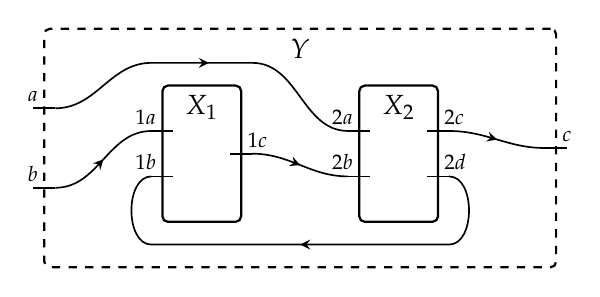
\begin{tikzpicture}[wiring diagram,baseline]
      \label{dia:string_diagram}
   \node[bb={2}{1}, bb name=$X_1$] (X1) {};
   \node[bb={2}{2}, right=of X1, bb name=$X_2$] (X2) {};
   \node[bb={2}{1}, dashed, fit={(X1) (X2) ($(X1.north)+(0,1.5)$) ($(X1.south)-(0,1)$)},
            bb name=$Y$] (Y) {};
   \draw[label]
      node[above left=of Y_in1]     {$a$}
      node[above left=of Y_in2]     {$b$}
      node[above right=of Y_out1]   {$c$}
      node[above left=of X1_in1]    {$1a$}
      node[above left=of X1_in2]    {$1b$}
      node[above right=of X1_out1]  {$1c$}
      node[above left=of X2_in1]    {$2a$}
      node[above left=of X2_in2]    {$2b$}
      node[above right=of X2_out1]  {$2c$}
      node[above right=of X2_out2]  {$2d$};
   \draw[ar] (Y_in2') to (X1_in1);
   \draw[ar] (X1_out1) to (X2_in2);
   \draw[ar] (X2_out1) to (Y_out1');
   \draw[ar] let \p1=(X1.north west), \p2=(X1.north east), \n1={\y1+\bby}, \n2=\bbportlen in
      (Y_in1') to (\x1-\n2,\n1) -- (\x2+\n2,\n1) to (X2_in1);
   \draw[ar] let \p1=(X2.south east), \p2=(X1.south west), \n1={\y1-\bby}, \n2=\bbportlen in
      (X2_out2) to[in=0] (\x1+\n2,\n1) -- (\x2-\n2,\n1) to[out=180] (X1_in2);
\end{tikzpicture}\end{equation}
represent compositions. That is, new morphisms are constructed from old by specifying which outputs
will be fed back into which inputs. In fact, these are related to Penrose diagrams in $\ncat{Vect}$,
and the word \emph{traced} originates in this vector space terminology~\cite{JoyalStreetVerity}.

\section{Traced string diagrams as cobordisms}
      \label{sec:traced_string_cob}

A string diagram usually does not explicitly include the outer box $Y$. If we include it, as in
(\ref{dia:string_diagram}), the resulting \emph{wiring diagram} can be given another interpretation:
it represents a 1-dimensional cobordism between oriented 0-manifolds. For example, the box $X_1$ in
the picture includes only the data of a pair of finite sets,
$(\inp{X_1},\outp{X_1})=(\{1a,1b\},\{1c\})$, which can be interpreted as an oriented 0-manifold.
Moreover, the wiring diagram itself, in which boxes $X_1,\ldots,X_n$ are wired together inside a
larger box $Y$, can be interpreted as an oriented cobordism from $X_1\sqcup\cdots\sqcup X_n$ to $Y$.
This is a morphism in the (colored) operad $\Cob$, underlying the symmetric monoidal category of
oriented 1-cobordisms; see Section~\ref{subsec:wds_and_cob}.

There is actually a bit more data in a string (or wiring) diagram for a traced category $\cat{C}$
than in a cobordism. Namely, each input and output of a box must be labeled by an object of
$\cat{C}$ and the wires connecting boxes must respect the labels (e.g., in
(\ref{dia:string_diagram}), object $2d$ must equal object $1b$). We will thus consider the operad
$\LCob{\LabSet}$ of oriented 1-dimensional cobordisms over a fixed set $\LabSet$ of labels.

In the table below, we record these two interpretations of a string diagram. Note the ``degree
shift'' between the second and third columns.
\begin{center} \begin{tabular}{lll}
   \toprule
      \multicolumn{3}{c}{Interpretations of string diagrams} \\
   \midrule
      String diagram & Traced category $\cat{C}$ & $\LCob{\LabSet}$ \\
   \midrule
      Wire label set, $\LabSet$ & Objects, $\LabSet\coloneqq\Ob(\cat{C})$ & Label set, $\LabSet$ \\
      Boxes, e.g., \tikz[wiring diagram,bb port sep=1,bby=2.4pt,bb min width=5.5pt,
                  bb port length=2pt,bb rounded corners=1pt,baseline=(B.south)]
               {\node[bb={1}{2}] (B) {};}
         & Morphisms in $\cat{C}$& Objects (oriented 0-mfds over $\LabSet$) \\
      String diagrams & Compositions in $\cat{C}$& Morphisms (cobordisms over $\LabSet$) \\
      Nesting & Axioms of traced cats & Composition (of cobordisms) \\
   \bottomrule
\end{tabular} \end{center}

\subsection{The formal connection between Cob-algebras and traced categories}
      \label{subsec:statement_of_main_thm}

The relationship between these interpretations of string diagrams is most easily made precise when
the set $\LabSet$ of labels is fixed. Let $\TTrCat$ (resp.\ $\TTrCatStrong$) denote the 2-category of
traced categories, traced strict (resp.\ strong) monoidal functors, and monoidal natural isomorphisms
\cite{HK}, and let $\TrCat$ denote the underlying 1-category of $\TTrCat$%
\footnote{
   We use a similar notational convention throughout this paper. We denote named 1-categories,
   monoidal categories, and operads with bold roman letters, e.g., $\ncat{Cob}$, and unnamed
   1-categories with script, e.g., $\cat{C}$. For named 2-categories or bicategories we do almost
   the same, but change the font of the first letter to calligraphic, such as $\nncat{T}{rCat}$; for
   unnamed 2-categories we use (unbold) calligraphic, e.g., $\ccat{D}$.  Finally, for equipments
   (special double categories, see Section~\ref{chap:background_equipments}) we make the first
   letter blackboard bold, whether named (e.g., $\ndcat{P}{rof}$) or unnamed (e.g., $\dcat{D}$). The
   objects in a category, 2-category, or double category will be denoted with the usual math font
   (e.g., $T\in\Ob\TrCat$). By the \emph{underlying 1-category} of a 2-category, we mean the one
   obtained by dropping (not quotienting by) the 2-cells.
}.
Finally, let $\TrCat_{\LabSet}$ denote the subcategory in which the monoid of objects is fixed to be
free on the set $\LabSet$, together with identity-on-objects functors.

For any monoidal category $\cat{M}$, we denote by $\cat{M}\alg\coloneqq\ncat{Lax}(\cat{M},\Set)$ the
category of lax functors $\cat{M}\to\Set$. Then there is an equivalence of categories
\begin{equation}
      \label{eq:single_fiber_tr}
   \LCob{\LabSet}\alg\equiv\TrCat_{\LabSet}.
\end{equation}
Some intuition for this statement will be given in Section~\ref{subsec:cobalg_and_trCat}, and it
will be generalized in \ref{thm:TheoremA_statement} and proven as such in Section~\ref{sec:deducing}.

\subsection{Compact categories vs.\ traced categories}

For each of our main results about traced categories in this paper, we will also prove an analogous
result about compact closed symmetric monoidal categories, hereafter \emph{compact categories}. The
definition of compact category can be found in Section~\ref{sec:compact_and_int}, or
in~\cite{MacL--CTWM}. Let $\CCompCat$ (resp.\ $\CCompCatStrong$) denote the 2-category of compact
categories with strict (resp.\ strong) functors, and let $\CompCat$ denote the underlying 1-category
of $\CCompCat$. As above, let $\CompCat_{\LabSet}$ denote the subcategory of compact categories
whose objects are free on the set $\LabSet$ (so the objects are strings such as $o_1o_2o_3^*$ of
labels $o_i\in\LabSet$ and their formal duals, and the tensor product is concatenation), together
with identity-on-objects functors.

There is an equivalence of categories
\begin{equation}
      \label{eq:single_fiber_comp}
   \LCob{\LabSet}\alg\equiv\CompCat_{\LabSet}.
\end{equation}
Equations \eqref{eq:single_fiber_tr} and \eqref{eq:single_fiber_comp} and the relationship between
them will be generalized in \ref{thm:TheoremA_statement}; see also \eqref{eqn:2pullbacks_1fiber}.

\section{The main results}
      \label{subsec:main_results}

The equivalence \eqref{eq:single_fiber_tr} (and likewise \eqref{eq:single_fiber_comp}) has two
drawbacks: the object set of the traced category is fixed, and it is assumed to be freely generated
by some set under tensor products (and duals, in the compact case); we refer to this later condition
using the term \emph{free-on-objects}. Much of the work in this paper is to relax these two
conditions. For the latter, we prove that the 2-category of traced categories and strong functors is
biequivalent to that of free-on-objects traced categories and strict functors; see
Corollary~\ref{cor:object_frees}. For the former, we first explain what kind of variance is
appropriate.

There are adjunctions
\[
   \Adjoint{\Set}{\TrCat}{\FT}{\UT}
   \qquad\text{and}\qquad
   \Adjoint{\Set}{\CompCat}{\FC}{\UC}
\]
which induce monads $\TT$ (respectively $\TC$) on $\Set$. The monad $\TT$ is in fact isomorphic to
the free monoid monad, while $\TC$ is isomorphic to the free monoid-with-involution monad.

Let $\cat{C}$ and $\cat{C}'$ be free-on-objects traced categories, such that $\Ob(\cat{C})$ is the free
monoid on a set $\LabSet$ and $\Ob(\cat{C}')$ is the free monoid on a set $\LabSet'$. A strict
(traced) monoidal functor $F\colon \cat{C}\to \cat{C}'$ induces a homomorphism
$\Ob F\colon\Ob(\cat{C})\to\Ob(\cat{C}')$ between the free monoids, or equivalently a function $\Ob
F\colon\LabSet\to\TT(\LabSet')$. Let $\Set_{\TT}$ denote the Kleisli category of this monad, so $\Ob
F$ is identified with a morphism in $\Set_{\TT}$. Likewise, if $\cat{C}$ and $\cat{C}'$ are
free-on-objects compact categories, then the object part $\Ob F$ of a strong functor
$F\colon\cat{C}\to\cat{C}'$ can be identified with a morphism in the Kleisli category $\Set_{\TC}$.

The compact category $\LCob{\LabSet}$ varies functorially in $\LabSet\in\Set$, and we will see later
that this functor extends to functors
\[
   (\LCob{\bullet})\colon\Set_{\TT}\to\CompCat\qquad\text{and}
   \qquad
   (\LCob{\bullet})\colon\Set_{\TC}\to\CompCat
\]
(see~\eqref{eqn:FMC}). We can compose these with $\Lax(-,\Set)$ to obtain functors which we denote
\begin{equation}
      \label{eqn:cob/bullet}
   (\LCob{\bullet})\alg\colon\Set_{\TT}^{\mathrm{op}}\too\Cat
   \qquad\text{and}\qquad
   (\LCob{\bullet})\alg\colon\Set_{\TC}^{\mathrm{op}}\too\Cat.
\end{equation}
By applying the Grothendieck construction to (\ref{eqn:cob/bullet}), we obtain fibrations for which
the fiber over a set $\LabSet$ is equivalent, using \eqref{eq:single_fiber_tr} and
\eqref{eq:single_fiber_comp}, to $\TrCat_{\LabSet}$ and $\CompCat_{\LabSet}$, respectively.

To state the next theorem, we give names to the categories described above. Let
\[
   \TTrFrObCat\ss\TTrCat \qquad \text{and} \qquad \CCompFrObCat\ss\CCompCat
\]
denote the full 2-subcategories spanned by the traced and compact categories (respectively) that are
free-on-objects. Let $\TrFrObCat$ and $\CompFrObCat$ (respectively) denote their underlying
1-categories.

\begin{named}{Theorem A}
      \label{thm:TheoremA_statement}
  There are equivalences of 1-categories
  \begin{align*}
     &\int^{\LabSet\in\Set_{\TT}}(\LCob{\LabSet})\alg \to \TrFrObCat
     \\
     &\int^{\LabSet\in\Set_{\TC}}(\LCob{\LabSet})\alg \to \CompFrObCat
  \end{align*}
\end{named}

The proof of this result can be found in Section~\ref{sec:deducing}. In order to see how the
free-on- objects traced (resp.\ compact) categories relate to general traced categories, we prove in
Appendix~\ref{appendix} the following result, which is well-known but difficult to find in the
literature:

\begin{corollary*}[\ref{cor:object_frees}]
   The canonical inclusions
   \begin{align*}
      \MMonFrObCat &\to \MMonCatStrong \\
      \TTrFrObCat &\to \TTrCatStrong \\
      \CCompFrObCat &\to \CCompCatStrong
   \end{align*}
   are biequivalences of 2-categories.
\end{corollary*}

Here $\MMonFrObCat$ and $\MMonCatStrong$ are defined analogously to the other two. See
Definition~\ref{def:free_on_objects}.

Our work in this direction leads to a characterization (see
Remark~\ref{rem:characterization_of_traced}) of the 2-category $\TTrCatStrong$ solely in terms of
$\MMonCatStrong$ and $\CCompCatStrong$---and the relationship between them---without mention of the
usual structures or axioms of traced categories as in \cite{JoyalStreetVerity}.

\begin{remark}
   The most naive way of handling variation of the label set $\LabSet$ is to use plain functions
   $\LabSet\to\LabSet'$. That is, instead of taking the Grothendieck construction of the functors
   \eqref{eqn:cob/bullet}, we could use the most evident functor
   $\Lax(\LCob{\bullet},\Set)\colon\op{\Set}\to\Cat$. This would lead to a version of
   \ref{thm:TheoremA_statement} in which the right hand side is a 2-category of ``traced colored
   PROPs''. We will not pursue this direction in the paper; however, the interested reader familiar
   with PROPs should have no difficulty defining traced colored PROPs and proving the analogue of
   \ref{thm:TheoremA_statement} as a corollary of our results. (For more on PROPs, see
   e.g.~\cite{HackneyRobertson}.)
\end{remark}

\subsection{Generalization: Lax algebras on compact categories}

In the course of proving \ref{thm:TheoremA_statement}, we will also prove a more general result
on lax functors $\cat{C}\to\Set$ for general compact categories $\cat{C}$.

We will see (in Theorem~\ref{thm:orthogonal} and Proposition~\ref{prop:CompProf_exact}) that there
is a factorization system on $\TrCat$, and similarly on $\CompCat$, in which the left class consists
of bijective-on-objects functors and the right class consists of fully faithful functors. Let
$\TrCat^{\bo}$ (resp.\ $\CompCat^{\bo}$) be the full subcategory of the arrow category $\TrCat^{\to}$
(resp.\ $\CompCat^{\to}$) spanned by the bijective-on-objects functors.

Using these factorization systems, we will see that the domain functors
\[
   \dom\colon\TrCat^{\bo}\twoheadrightarrow\TrCat
   \qquad\text{and}\qquad
   \dom\colon\CompCat^{\bo}\twoheadrightarrow\CompCat
\]
are fibrations. For a fixed traced category $\cat{T}$, the fiber
$\TrCat^{\bo}_{\cat{T}/}\coloneqq\dom^{-1}(\cat{T})$ is the category of strict monoidal,
bijective-on-objects functors from $\cat{T}$ to another traced category, with the evident
commutative triangles as morphisms, and likewise for $\CompCat^{\bo}_{\cat{C}/}$ with $\cat{C}$ a
compact category. Note that we have isomorphisms $\TrCat_{\LabSet}\iso\TrCat^{\bo}_{(\FT\LabSet)/}$
and $\CompCat_{\LabSet}\iso\CompCat^{\bo}_{(\FC\LabSet)/}$.

Recall from~\cite{JoyalStreetVerity} that traced categories can be thought of as full subcategories
of compact categories.  The Int construction, applied to a traced category $\cat{C}$, returns the
smallest compact category $\Int(\cat{C})$ of which it is a monoidal subcategory. We will recall these
notions in Sections~\ref{sec:intuition_for_traced} and~\ref{sec:compact_and_int}.

Generalizing \eqref{eq:single_fiber_tr} and \eqref{eq:single_fiber_comp}, we can give a complete
characterization of lax functors out of compact categories. For a fixed traced category $\cat{T}$
and a fixed compact category $\cat{C}$, there are equivalences of categories
\begin{equation}
      \label{eqn:lax_compcat_bo}
   \Lax(\Int(\cat{T}),\Set)\equiv\TrCat^{\bo}_{\cat{T}/}
   \qquad\text{and}\qquad
   \Lax(\cat{C},\Set)\equiv\CompCat^{\bo}_{\cat{C}/}.
\end{equation}
We will prove the following theorem in Section~\ref{sec:deducing}, generalizing
\ref{thm:TheoremA_statement}:

\begin{named}{Theorem B}
      \label{thm:TheoremB_statement}
   There are equivalences of fibrations
   \begin{equation*}
      \begin{tikzcd}[column sep=-1em]
         \int\limits^{\mathclap{\cat{C}\in\TrCat}} \Lax(\Int(\cat{C}),\Set)
               \ar[rr,"\equiv"] \ar[dr,two heads]
            && \TrCat^{\bo} \ar[dl,two heads,"\dom" pos=.4] \\
         & \TrCat &
      \end{tikzcd}
      \qquad\text{and}\qquad
      \begin{tikzcd}[column sep=-1em]
         \int\limits^{\mathclap{\cat{C}\in\CompCat}} \Lax(\cat{C},\Set)
               \ar[rr,"\equiv"] \ar[dr,two heads]
            && \CompCat^{\bo} \ar[dl,two heads,"\dom" pos=.4] \\
         & \CompCat &
      \end{tikzcd}
   \end{equation*}
\end{named}

We can give a better high-level story once we have reviewed \emph{equipments}; see the introduction
to Section~\ref{chap:equipments_monoidal_profunctors}. For the remainder of the introduction, we
will attempt to build intuition.

\section{Wiring Diagrams, cobordisms, and traced categories}

In this section, we give a bit more intuition about the connection between wiring diagrams and
cobordisms, and the equivalence between the category of traced categories and the category of
cobordism algebras.

\subsection{Wiring diagrams and $\Cob$}
      \label{subsec:wds_and_cob}

The objects in $\Cob$ are signed sets $(\inp{X},\outp{X})$, each of which can be drawn as a box with
input wires $\inp{X}$ drawn entering the box, on its left, and output wires $\outp{X}$ drawn exiting
the box, on its right. For the time being, we call the latter style \emph{an interface}.

\begin{equation*}
   \begin{tikzpicture}[node distance=0 and 0, baseline=(current bounding box.center)]
      \node (A1) {$-$};
      \node[below=-.1 of A1] (A2) {$-$};
      \node[below=-.1 of A2] (A3) {$-$};
      \node[below=-.1 of A3] (B1) {$+$};
      \node[below=-.1 of B1] (B2) {$+$};
   \end{tikzpicture}
   \hspace{4em}
   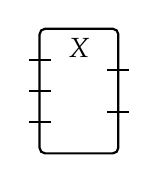
\begin{tikzpicture}[wiring diagram, bby=1.2ex, baseline=(current bounding box.center)]
      \node[bb={3}{2},bb name=$X$] {};
   \end{tikzpicture}
\end{equation*}

Wiring diagrams seem to be a new way to visualize morphisms in the symmetric monoidal category
$\Cob$ of 1-dimensional oriented cobordisms. In fact, they are better suited to the operad
associated to $\Cob$. The following shows the two approaches to drawing a 2-ary morphism $X_1,X_2\to
Y$:

\begin{equation*}
   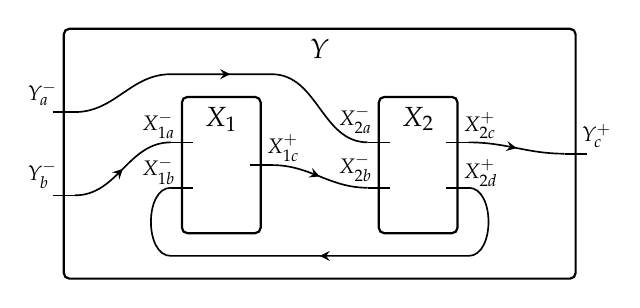
\begin{tikzpicture}[wiring diagram, baseline=(current bounding box.center)]
      \node[bb={2}{1}, bb name=$X_1$] (X1) {};
      \node[bb={2}{2}, right=of X1, bb name=$X_2$] (X2) {};
      \node[bb={2}{1}, fit={(X1) (X2) ($(X1.north)+(0,2)$) ($(X1.south)-(0,1)$)},bb name =$Y$] (Y) {};
      \draw[label]
          node[above left=of Y_in1]     {$\inp{Y}_a$}
          node[above left=of Y_in2]     {$\inp{Y}_b$}
          node[above right=of Y_out1]   {$\outp{Y}_c$}
          node[above left=1pt and -2pt of X1_in1]    {$\inp{X}_{1a}$}
          node[above left=1pt and -2pt of X1_in2]    {$\inp{X}_{1b}$}
          node[above right=1pt and -2pt of X1_out1]  {$\outp{X}_{1c}$}
          node[above left=3pt and -2pt of X2_in1]    {$\inp{X}_{2a}$}
          node[above left=2pt and -2pt of X2_in2]    {$\inp{X}_{2b}$}
          node[above right=1pt and -2pt of X2_out1]  {$\outp{X}_{2c}$}
          node[above right=0pt and -2pt of X2_out2]  {$\outp{X}_{2d}$};
      \draw[ar] (Y_in2') to (X1_in1);
      \draw[ar] (X1_out1) to (X2_in2);
      \draw[ar] (X2_out1) to (Y_out1');
      \draw[ar] let \p1=(X1.north west), \p2=(X1.north east), \n1={\y1+\bby}, \n2=\bbportlen in
          (Y_in1') to (\x1-\n2,\n1) -- (\x2+\n2,\n1) to (X2_in1);
      \draw[ar] let \p1=(X2.south east), \p2=(X1.south west), \n1={\y1-\bby}, \n2=\bbportlen in
         (X2_out2) to[in=0] (\x1+\n2,\n1) -- (\x2-\n2,\n1) to[out=180] (X1_in2);
   \end{tikzpicture}
   \qquad
   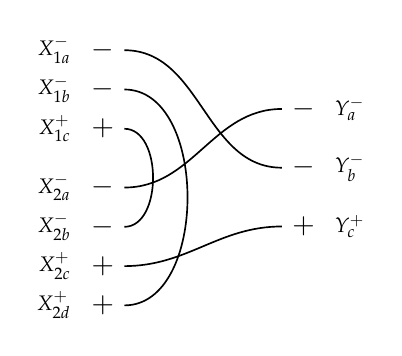
\begin{tikzpicture}[x=1cm,y=1ex,node distance=1 and 1,semithick,every label quotes/.style={font=\everymath\expandafter{\the\everymath\scriptstyle}},every to/.style={out=0,in=180},baseline=(current bounding box.center)]
      \node ["$\inp{X}_{1a}$" left] (X1a) {$-$};
      \node [below=0 of X1a, "$\inp{X}_{1b}$" left] (X1b) {$-$};
      \node [below=0 of X1b, "$\outp{X}_{1c}$" left] (X1c) {$+$};
      \node [below=1.5 of X1c, "$\inp{X}_{2a}$" left] (X2a) {$-$};
      \node [below=0 of X2a, "$\inp{X}_{2b}$" left] (X2b) {$-$};
      \node [below=0 of X2b, "$\outp{X}_{2c}$" left] (X2c) {$+$};
      \node [below=0 of X2c, "$\outp{X}_{2d}$" left] (X2d) {$+$};
      \node [below right=1.5 and 2 of X1a, "$\inp{Y}_a$" right] (Ya) {$-$};
      \node [below=1.5 of Ya, "$\inp{Y}_b$" right] (Yb) {$-$};
      \node [below=1.5 of Yb, "$\outp{Y}_c$" right] (Yc) {$+$};
      \draw (X1a) to (Yb);
      \draw (X1b) to[in=0] (X2d);
      \draw (X1c) to[in=0] (X2b);
      \draw (X2a) to (Ya);
      \draw (X2c) to (Yc);
   \end{tikzpicture}
\end{equation*}

\subsection{$\Cob$-algebras and traced categories}
      \label{subsec:cobalg_and_trCat}

Here we sketch the equivalence of categories
\[
   \LCob{\LabSet}\alg\equiv\TrCat_{\LabSet}
\]
from Section~\ref{subsec:statement_of_main_thm}. We will see that the same data are required, and
the same conditions are satisfied, whether one is specifying a lax functor $P\in\LCob{\LabSet}\alg$
or a traced category $\cat{C}\in\TrCat_{\LabSet}$ with objects generated by a set $\LabSet$.

First, for each box $X=(\inp{X},\outp{X})$ that might appear in a string diagram, both
$P\colon\LCob{\LabSet}\to\Set$ and $\cat{C}$ require a set, $P(X)$ and
$\Hom_{\cat{C}}(\inp{X},\outp{X})$, respectively. Second, for each string diagram, both $P$ and
$\cat{C}$ require a function: an action on morphisms, in the case of $P$, and a formula for
performing the required compositions, tensors, and traces, in the case of $\cat{C}$. The condition
that $P$ is functorial corresponds to the fact that $\cat{C}$ satisfies the axioms of traced
categories.

We will briefly specify how to construct a lax functor $P$ from a traced category
$(\cat{C},\otimes,I,\Tr)$, whose objects are freely generated by $\LabSet$. We will abuse notation
slightly as follows: Given a relative set $\iota\colon Z\to\LabSet$, we will use the same symbol $Z$
to denote the tensor $\bigotimes_{z\in Z}\iota(z)$ in $\cat{C}$.

For an oriented 0-manifold $X=\inp{X}\sqcup \outp{X}$ over $\LabSet$, we set
$P(X)\coloneqq\Hom_{\cat{C}}(\inp{X},\outp{X})$. Given a cobordism $\Phi\colon X\to Y$, we need a
function $P(\Phi)\colon P(X)\to P(Y)$. For any cobordism $\Phi$, there exist
$A,B,C,D,E\in\Ob\cat{C}$ such that $\inp{X}\cong C\otimes A$, $\outp{X}\cong C\otimes B$,
$\inp{Y}\cong A\otimes D$, $\outp{Y}\cong B\otimes D$, and $E$ is the set of floating loops in
$\Phi$; thus $\Phi$ is essentially equivalent to the cobordism shown on the right side of
(\ref{eq:cob_and_trace_pic}).
\begin{equation}
      \label{eq:cob_and_trace_pic}
   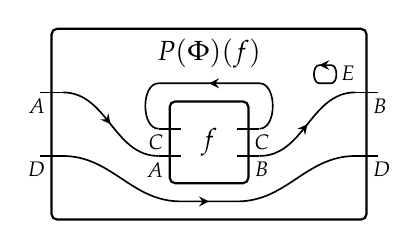
\begin{tikzpicture}[wiring diagram, bby=1.4ex, baseline=(current bounding box.center)]
      \node[bb port sep=1.5, bb={2}{2}] (domain) {$f$};
      \node[bb={2}{2}, fit={(domain) ($(domain.north)+(0,3)$) ($(domain.south)-(0,1)$)}, bb name=$P(\Phi)(f)$] (codomain) {};
      \draw[ar] (codomain_in1') to (domain_in2);
      \draw[ar] (domain_out2) to (codomain_out1');
      \draw[ar] let \p1=(domain.north east), \p2=(domain.north west), \n1={\y1+\bby}, \n2=\bbportlen in
          (domain_out1) to[in=0] (\x1+\n2,\n1) -- (\x2-\n2,\n1) to[out=180] (domain_in1);  %Trace on C
      \draw[ar] let \p1=(domain.south west), \p2=(domain.south east), \n1={\y1-\bby}, \n2=\bbportlen in
          (codomain_in2') to[in=180] (\x1+\n2,\n1) -- (\x2-\n2,\n1) to[out=0] (codomain_out2'); %Identity on D
      \draw[ar] let \p1=(domain.north east) in
          (\x1+.7*\bbx,\y1+\bby) to[in=0] (\x1+.7*\bbx,\y1+2*\bby) -- (\x1+.6*\bbx,\y1+2*\bby) to[out=180] (\x1+.6*\bbx,\y1+\bby) -- (\x1+.7*\bbx,\y1+\bby);%Loop
      \draw[label] let \p1=(domain.north east) in
          node[below left=of codomain_in1]     {$A$}
          node[below left=of codomain_in2]     {$D$}
          node[below right=of codomain_out1]    {$B$}
          node[below right=of codomain_out2]    {$D$}
          node[above left=.6 and 0 of codomain_out1']  {$E$}
          node[below left=of domain_in1]     {$C$}
          node[below left=of domain_in2]     {$A$}
          node[below right=of domain_out2]    {$B$}
          node[below right=of domain_out1]   {$C$};
   \end{tikzpicture}
   \qquad\qquad
   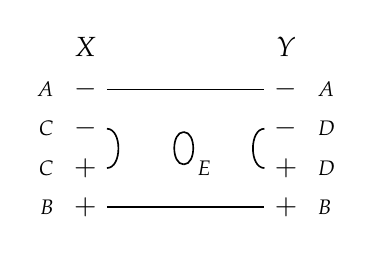
\begin{tikzpicture}[x=1cm,y=1ex,node distance=1 and 1,semithick,every label quotes/.style={font=\everymath\expandafter{\the\everymath\scriptstyle}},every to/.style={out=0,in=180},baseline=(current bounding box.center)]
      \node ["$A$" left] (X1a) {$-$};
      \node [above=0.25 of X1a] {$X$};
      \node [below=0 of X1a, "$C$" left] (X1b) {$-$};
      \node [below=0 of X1b, "$C$" left] (X2a) {$+$};
      \node [below=0 of X2a, "$B$" left] (X2b) {$+$};
      \node [right=2 of X1a, "$A$" right] (Y1a) {$-$};
      \node [above=0.25 of Y1a] {$Y$};
      \node [below=0 of Y1a, "$D$" right] (Y1b) {$-$};
      \node [below=0 of Y1b, "$D$" right] (Y2a) {$+$};
      \node [below=0 of Y2a, "$B$" right] (Y2b) {$+$};
      \node [right=1.45 of X2a, "$E$" left] {};
      \draw (X1a) to (Y1a);
      \draw (X1b) to[in=0] (X2a);
      \draw (X2b) to (Y2b);
      \draw (Y1b) to[in=180,out=180] (Y2a);
      \draw ($(X1b)+(1.25,-2.75)$) to[in=0] ($(X1b)+(1.25,-0.25)$);
      \draw ($(X1b)+(1.25,-0.25)$) to[in=180,out=180] ($(X1b)+(1.25,-2.75)$);
   \end{tikzpicture}
\end{equation}
With the above notation, for $f\in P(X)$ we can follow the string diagram (left of
(\ref{eq:cob_and_trace_pic})) and define
\begin{equation}
      \label{eq:cob algebra formula}
   P(\Phi)(f)\coloneqq\Tr_{A,B}^C[f]\otimes D\otimes\Tr^E_{I,I}[\id_E].
\end{equation}


\section{Applications of the operadic perspective}

The operadic perspective on traced categories may be useful in concrete applications, such as for
modeling nested process diagrams. It may also be useful in pure mathematics, because the operad $\Cob$,
which indexes traced categories, can be easily modified to model a variety of other doctrines.
These two applications will be discussed in more detail in
Sections~\ref{subsec:modular}~and~\ref{subsec:math_application} respectively.

\subsection{Modular design}
      \label{subsec:modular}

When designing or investigating a complex system, it is often useful to think in terms of
interacting subsystems, put together to make a larger whole. In manufacturing, this is often called
\emph{modular design}. Each object in $\Cob$ represents an interface, or \emph{module}, with a
fixed number and type of inputs and outputs. The morphisms in $\Cob$ correspond to strategies by
which these interfaces can be wired together into a process, which itself has an interface (the outer box).

An algebra $P\colon\Cob\to\Set$ provides semantics for these interfaces
(\cite{RupelSpivak},\cite{VagnerSpivakLerman}). For each interface $X$, the set $P(X)$ represents
the set of possible ``fillers'' for it. For example, one might imagine that each interface $X$ can
be filled by any state machine having that interface; in this case $P(X)$ would be the set of such
state machines. For a morphism $\varphi\colon X_1,\ldots,X_n\to Y$, the function $P(\varphi)$ tells
us how to construct a filler of interface $Y$, given fillers on each $X_i$. Composition of
cobordisms are drawn as nested diagrams:
\begin{equation*} 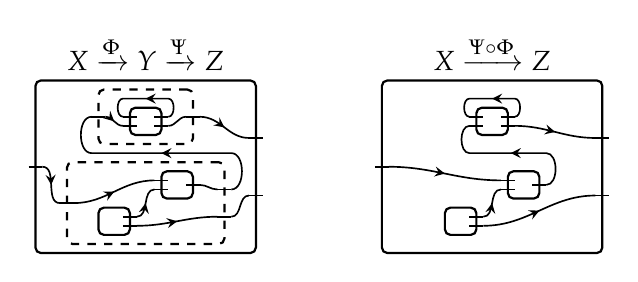
\begin{tikzpicture}[wiring diagram, bb small]
   \node[bb={2}{2}] (X1) {};
   \node[bb={1}{1}, fit={(X1) ($(X1.north)+(0,1)$)}, dashed] (Y1) {};
   \node[bb={2}{1}, below right=4 and 0 of X1] (X2) {};
   \node[bb={0}{2},below left=of X2] (X3) {};
   \node[bb={1}{2}, fit=(X2) (X3), dashed] (Y2) {};
   \node[bb={1}{2}, fit=(Y1) (Y2)] (Z) {};
   \draw[ar] (Z_in1') to (Y2_in1);
   \draw[ar] (Y2_in1') to (X2_in1);
   \draw[ar] (X3_out1) to (X2_in2);
   \draw[ar] (X3_out2) to (Y2_out2');
   \draw (Y2_out2) to (Z_out2');
   \draw[ar] (Y1_in1') to (X1_in2);
   \draw (X1_out2) to (Y1_out1');
   \draw[ar] (Y1_out1) to (Z_out1');
   \draw (X2_out1) to (Y2_out1');
   \draw[ar] let \p1=(Y2.north east), \p2=(Y1.south west), \n1={\y1+\bby}, \n2=\bbportlen in
      (Y2_out1) to[in=0] (\x1+\n2,\n1) -- (\x2-\n2,\n1) to[out=180] (Y1_in1);
   \draw[ar] let \p1=(X1.north east), \p2=(X1.north west), \n1={\y1+\bby}, \n2=\bbportlen in
      (X1_out1) to[in=0] (\x1+\n2,\n1) -- (\x2-\n2,\n1) to[out=180] (X1_in1);
   \node[anchor=south] at (Z.north) {$X\xrightarrow{\Phi}Y\xrightarrow{\Psi}Z$};

   \node[bb={2}{2}, right=10 of X1] (X1') {};
   \node[bb={2}{1}, below right=4 and 0 of X1'] (X2') {};
   \node[bb={0}{2},below left=of X2'] (X3') {};
   \node[bb={1}{2}, fit={($(X1'.north)+(0,1)$) (X2') (X3')}, inner xsep=2*\bbx, inner ysep=2*\bby] (Z') {};
   \draw[ar] (X3'_out1) to (X2'_in2);
   \draw[ar] (Z'_in1') to (X2'_in1);
   \draw[ar] (X1'_out2) to (Z'_out1');
   \draw[ar] (X3'_out2) to (Z'_out2');
   \draw[ar] let \p1=(X2'.north east), \p2=(X1'.south west), \n1={\y1+2*\bby}, \n2=\bbportlen in
      (X2'_out1) to[in=0] (\x1+\n2,\n1) -- (\x2-\n2,\n1) to[out=180] (X1'_in2);
   \draw[ar] let \p1=(X1'.north east), \p2=(X1'.north west), \n1={\y1+\bby}, \n2=\bbportlen in
      (X1'_out1) to[in=0] (\x1+\n2,\n1) -- (\x2-\n2,\n1) to[out=180] (X1'_in1);
   \node[anchor=south] at (Z'.north) {$X\xrightarrow{\Psi\circ\Phi}Z$};
\end{tikzpicture} \end{equation*}

In our model for modular design, any way to chunk the small boxes inside the big one will yield the
same result. This is a reflection of the functoriality of $P\colon\Cob\to\Set$, which says that
commutative diagrams in $\Cob$ are sent to commutative diagrams of sets. Nested structures, given
by composition of such morphisms, may be useful for the kind of chunking that humans use to
understand complex systems~\cite{Miller}.

\subsection{Mathematical application: varying the operad}
      \label{subsec:math_application}

Formalizing modular design using operads, as in~\cite{Spivak},~\cite{RupelSpivak},
and~\cite{VagnerSpivakLerman} was the original motivation for the present paper, as the drawings had
strong similarities to those found in traced categories. However, it should be noted that none of
these papers actually uses $\Cob$ as the indexing category for their algebras, and hence none are
actually directly related to traced categories. In fact, they use three different operads, of
varying degrees of similarity to $\Cob$. For example, there is an orthogonal factorization system on
$\Cob$ \cite{Abadi}, for which morphisms in the left class $\cat{L}$ include no closed loops, and
the operad of interest in~\cite{VagnerSpivakLerman} is $\cat{L}$.

If one wished to make minor modifications in the axioms of traced categories to create some new sort
of category $\ncat{Tr'Cat}$, one may proceed by imagining the string diagrams that should describe
compositions in $\ncat{Tr'Cat}$. For example, one may want to consider cartesian traced categories,
in which wires can split or terminate abruptly. Or one might want to allow splitting but not allow
abrupt termination.
\begin{equation*} 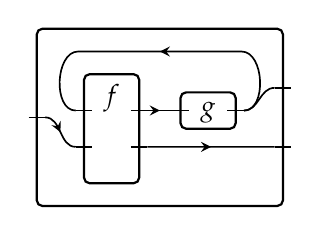
\begin{tikzpicture}[wiring diagram,bb min width =.7cm, bb port sep =1, bbx=.6cm,bb port length=3pt]
   \node[bb port sep=1.6, bb={2}{2}, bb name=$f$] (X1) {};
   \node[bb port sep=.8,bb={1}{1}, right=.7 of X1_out1, bb name=$g$] (X2) {};
   \node[bb={1}{2}, fit={(X1) (X2) ($(X1.north)+(0,1)$)}] (Y) {};
   \draw[ar] (Y_in1') to (X1_in2);
   \draw[ar,pos=.8] (X1_out1) to (X2_in1);
   \draw (X2_out1) to (Y_out1');
   \draw[ar] (X1_out2) to (Y_out2');
   \draw[ar] let \p1=(X2.north east), \p2=(X1.north west), \n1={\y2+\bby}, \n2=\bbportlen in
      (X2_out1) to[in=0] (\x1+.7*\n2,\n1) -- (\x2-.7*\n2,\n1) to[out=180] (X1_in1);
\end{tikzpicture} \end{equation*}
There is sometimes a tension between identity morphisms and the trace structure, e.g., if the
morphisms are dynamical systems. Imagining the wiring diagrams for traced categories without
identities is straightforward (the relevant operad is $\cat{L}$ above), whereas determining the
relevant axiomatization for them is not. An approach to this issue was suggested in \cite{ABP}, in
which traced categories without identities are embedded in larger categories as ``trace ideals";
however, it may sometimes be preferable to work with the category on its own terms.

We can accommodate any of the above such modification of string diagrams for $\ncat{Tr'Cat}$ by
modifying the indexing operad $\Cob$ to some operad $\Cob'$. Using $\cat{L}$ for dynamical systems
in \cite{VagnerSpivakLerman} is an example of this. As another, suppose that, as above, we want
string diagrams in which wires can split but not terminate. Noting that an oriented cobordism
$\varphi$ includes the data of a function
\begin{equation*}
   \varphi\colon\inp{X}\sqcup\outp{Y}\to\outp{X}\sqcup\inp{Y},
\end{equation*}
which is both injective and surjective, we can obtain the desired indexing operad $\Cob'$ by
requiring surjectivity but not injectivity in $\varphi$. These were found to be useful in
\cite{RupelSpivak}.

\section{Plan of the paper}

In Section~\ref{chap:traced_categories} we review monoidal, traced, and compact categories, as well
as the notion of orthogonal factorization systems. In Section~\ref{chap:background_equipments} we
review equipments (also known as framed bicategories) \cite{Shulman}, and exact equipments
\cite{Schultz2015}. In Section~\ref{sec:internal_presheaves} we record the definition of
copresheaves internal to an equipment, which we need to properly express our main theorems. We
finally introduce the equipments of primary interest, $\dMonProf, \dTrProf$, and $\dCompProf$ in
Section~\ref{chap:equipments_monoidal_profunctors}. We prove that they are exact in
Section~\ref{sec:exactness_proofs} and, in Section~\ref{sec:special_CompProf}, we prove the special
properties about $\dCompProf$ which are at the core of our results. Indeed one might view the rest
of the paper as a formal wrapper for the results in that section. In
Section~\ref{sec:monoids_on_free} we deal with freeness-on-objects, which we need for
\ref{thm:TheoremA}. We deduce it as well as \ref{thm:TheoremB} in Section~\ref{sec:deducing}. The
appendix contains material that is not necessary to the paper. Its function is to prove a
biequivalence between the 2-category $\MMonCatStrong$ of monoidal categories with arbitrary object
set and strong functors, on the one hand, and the 2-category $\MMonFrObCat$ of monoidal categories
with free object set and strict functors. We do the same for traced and compact categories, all in
Corollary~\ref{cor:object_frees}.

\section*{Acknowledgments}

Thanks go to Steve Awodey and Ed Morehouse for suggesting we formally connect the operad-algebra
picture in \cite{RupelSpivak} to string diagrams in traced categories. We also thank Mike Shulman
for many useful conversations, and Tobias Fritz, Justin Hilburn, and Dmitry Vagner for helpful
comments on drafts of this paper.

\chapter{Categorical preliminaries}
      \label{chap:traced_categories}

In this section we remind the reader of some categorical preliminaries. Basic definitions and facts
about monoidal, traced, and compact categories, lax and strong functors, and the Int construction
are given in Sections~\ref{sec:prelim_monoidal}~through~\ref{sec:compact_and_int}. The fact that the
free compact category on a set has an algebraic description in terms signed sets and bijections, and
the fact that it has a geometric description in terms of 1-dimensional oriented cobordisms is
recalled in Section~\ref{sec:free_and_geometry}. In Section~\ref{sec:factorization_systems} we
review orthogonal factorization systems in categories and strict 2-categories.

\section{Monoidal categories}
      \label{sec:prelim_monoidal}

Recall that a \emph{strict monoidal category} $\cat{C}$ is a category equipped with a functor
$\otimes\colon\cat{C}\times\cat{C}\to\cat{C}$ and an object $I\in\cat{C}$, satisfying the usual
monoid axioms. In other words, a strict monoidal category is a monoid object in the category $\Cat$.
The category $\cat{C}$ is \emph{symmetric strict monoidal} if there is in addition a natural
isomorphism
\[
   \sigma_{X,Y}\colon X\otimes Y\to Y\otimes X
\]
satisfying equations $\sigma_{X,Y\otimes Z}=(\id_X\otimes\sigma_{X,Z})\circ(\sigma_{X,Y}\otimes
\id_Z)$ and $\sigma_{Y,X}\circ\sigma_{X,Y}=\id_{X\otimes Y}$.

Let $\cat{C}$ and $\cat{D}$ be monoidal categories. Recall that a functor
$F\colon\cat{C}\to\cat{D}$ is called \emph{lax monoidal} if it is equipped with a morphism
\begin{equation*} \begin{tikzcd}
      I_D \rar{\mu} & F(I_C)
\end{tikzcd} \end{equation*}
and a natural transformation
\begin{equation*} \begin{tikzcd}
      F(X) \otimes_D F(Y) \rar{\mu_{X,Y}} & F(X\otimes_C Y)
\end{tikzcd} \end{equation*}
satisfying some equations (see, e.g., \cite{Leinster,BorceuxV2}). The $\mu$'s are called
\emph{coherence morphisms}. If $\cat{C}$ and $\cat{D}$ are symmetric monoidal, then $F$ is \emph{lax
symmetric monoidal} if the coherence morphisms respect $\sigma$ in the appropriate way. If all
coherence morphisms are isomorphisms, then $F$ is \emph{strong}, and if they are all identities,
then $F$ is \emph{strict}.

Let $\MMonCat$ denote the 2-category of symmetric strict monoidal categories, strict symmetric
monoidal functors, and monoidal transformations, and let $\MonCat$ denote the underlying 1-category.
Let $\Lax(\cat{C},\cat{D})$ denote the category of lax monoidal functors and monoidal
transformations from $\cat{C}$ to $\cat{D}$.

\begin{warning}
      \label{warn:symmetric}
   For the rest of this article, whenever we discuss monoidal categories, we will mean symmetric
   strict monoidal categories. For example, see the definition of $\MMonCat$ above.
\end{warning}

\section{Traced categories}
      \label{sec:intuition_for_traced}

A \emph{trace structure} on a (symmetric strict) monoidal category $\cat{M}$ is a collection of
functions
\begin{equation}
      \label{dia:trace function}
   \Tr^U_{X,Y}\colon\Hom_{\cat{M}}(U\otimes X,U\otimes Y)\to\Hom_{\cat{M}}(X,Y)
\end{equation}
for $U,X,Y\in\Ob(\cat{M})$ satisfying seven equational axioms. When traced categories are defined,
e.g., in \cite{JoyalStreetVerity}, one often sees the trace functions, as well as each of the
axioms, accompanied by a picture. For example, (\ref{dia:trace function}) applied to an arbitrary
morphism $f\colon U\otimes X\to U\otimes Y$ might be accompanied by this picture:
\begin{equation*} 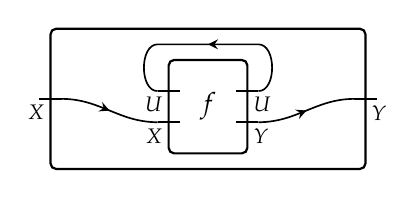
\begin{tikzpicture}[wiring diagram,bby=1.2ex]
      \node[bb={2}{2}] (domain) {$f$};
      \node[bb={1}{1}, fit={(domain) ($(domain.north)+(0,1)$)}] (codomain) {};
      \draw[ar] (codomain_in1') to (domain_in2);
      \draw[ar] (domain_out2) to (codomain_out1');
      \draw[ar] let \p1=(domain.north east), \p2=(domain.north west), \n1={\y1+\bby}, \n2=\bbportlen in
         (domain_out1) to[in=0] (\x1+\n2,\n1) -- (\x2-\n2,\n1) to[out=180] (domain_in1);
      \draw[label]
          node[below left=of codomain_in1]     {$X$}
          node[below right=of codomain_out1]    {$Y$}
          node[below left=of domain_in1]     {$U$}
          node[below left=of domain_in2]     {$X$}
          node[below right=of domain_out2]    {$Y$}
          node[below right=of domain_out1]   {$U$};
\end{tikzpicture} \end{equation*}
This can be recognized as a cobordism between oriented 0-manifolds, as we discussed in
Section~\ref{subsec:wds_and_cob}. Each of the seven axioms is vacuous from this perspective, in the
sense that both sides of the equation correspond to the same cobordism (up to diffeomorphism). For
example, here are the axioms of \emph{dinaturality} and \emph{superposition}:
\begin{itemize}
   \item For every $f\colon U\otimes X\to V\otimes Y$ and $g:V\to U$ we have
      \[
         \Tr^U_{X,Y}\Big[\big(g\otimes Y\big)\circ f\Big]=\Tr^V_{X,Y}\Big[f\circ\big(g\otimes X\big)\Big];
      \]
      \[\tikzset{bbx=1cm}
         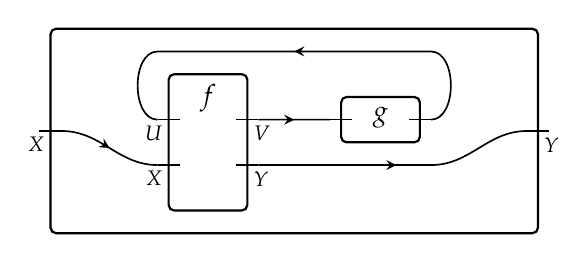
\begin{tikzpicture}[wiring diagram,baseline=(current bounding box.center)]
            \node[bb={2}{2}, bb name=$f$] (X1) {};
            \node[bb port sep=1,bb={1}{1}, right=.7 of X1_out1, bb name=$g$] (X2) {};
            \node[bb={1}{1}, fit={(X1) (X2) ($(X1.north)+(0,1)$)}] (Y) {};
            \draw[ar] (Y_in1') to (X1_in2);
            \draw[ar,pos=.8] (X1_out1) to (X2_in1);
            \draw[ar] let \p1=(X2.south east), \n1={\y1-\bby}, \n2=\bbportlen in
                (X1_out2) -- (\x1+\n2,\n1) to (Y_out1');
            \draw[ar] let \p1=(X2.north east), \p2=(X1.north west), \n1={\y2+\bby}, \n2=\bbportlen in
                  (X2_out1) to[in=0] (\x1+\n2,\n1) -- (\x2-\n2,\n1) to[out=180] (X1_in1);
            \draw[label]
                node[below left=of Y_in1]     {$X$}
                node[below right=of Y_out1]    {$Y$}
                node[below left=of X1_in1]     {$U$}
                node[below left=of X1_in2]     {$X$}
                node[below right=of X1_out2]    {$Y$}
                node[below right=of X1_out1]   {$V$};
         \end{tikzpicture}
         \quad=\quad
         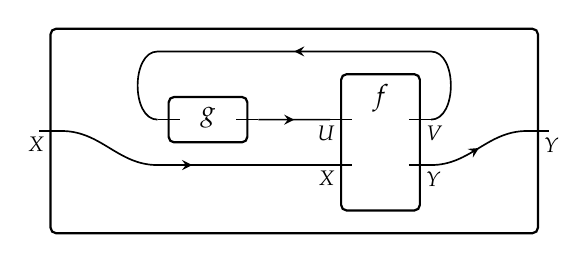
\begin{tikzpicture}[wiring diagram,baseline=(current bounding box.center)]
            \node[bb={2}{2}, bb name=$f$] (X1) {};
            \node[bb port sep=1,bb={1}{1}, left=.7 of X1_in1, bb name=$g$] (X2) {};
            \node[bb={1}{1}, fit={(X1) (X2) ($(X1.north)+(0,1)$)}] (Y) {};
            \draw[ar] let \p1=(X2.south west), \n1={\y1-\bby}, \n2=\bbportlen in
                (Y_in1') to (\x1-\n2,\n1) -- (X1_in2);
            \draw[ar] (X2_out1) to (X1_in1);
            \draw[ar] (X1_out2) to (Y_out1');
            \draw[ar] let \p1=(X1.north east), \p2=(X2.north west), \n1={\y1+\bby}, \n2=\bbportlen in
                  (X1_out1) to[in=0] (\x1+\n2,\n1) -- (\x2-\n2,\n1) to[out=180] (X2_in1);
            \draw[label]
                node[below left=of Y_in1]     {$X$}
                node[below right=of Y_out1]    {$Y$}
                node[below left=of X1_in1]     {$U$}
                node[below left=of X1_in2]     {$X$}
                node[below right=of X1_out2]    {$Y$}
                node[below right=of X1_out1]   {$V$};
         \end{tikzpicture}
         \]
   \item For every $f\colon U\otimes X\to U\otimes Y$ and $g\colon W\to Z$ we have
      \[
         \Tr^U_{X,Y}\big[f\big]\otimes g=\Tr^U_{X\otimes W,Y\otimes Z}\big[f\otimes g\big];
      \]
      \[\tikzset{bbx=.8cm,bb port sep=1.5}
      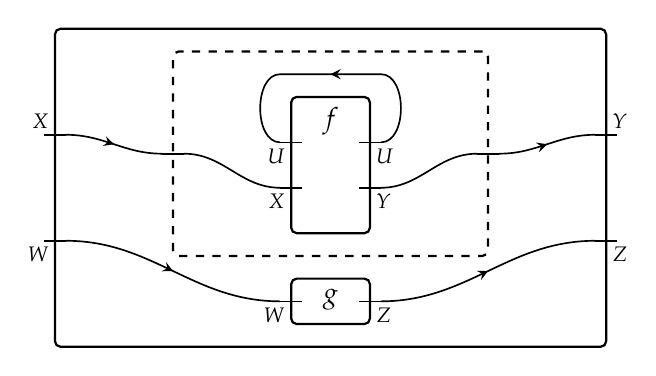
\begin{tikzpicture}[wiring diagram,baseline=(current bounding box.center)]
         \node[bb={2}{2}, bb name=$f$] (X1) {};
         \node[bb port sep=1,bb={1}{1}, below=2 of X1, bb name=$g$] (X2) {};
         \node[bb={1}{1}, fit={(X1) ($(X1.north)+(0,1)$)}, dashed] (Z) {};
         \node[bb={2}{2}, fit={(Z) (X2)}] (Y) {};
         \draw[ar] (Y_in1') to (Z_in1);
         \draw (Z_in1') to (X1_in2);
         \draw[ar] (Y_in2') to (X2_in1);
         \draw (X1_out2) to (Z_out1');
         \draw[ar] (Z_out1) to (Y_out1');
         \draw[ar] (X2_out1) to (Y_out2');
         \draw[ar] let \p1=(X1.north east), \p2=(X2.north west), \n1={\y1+\bby}, \n2=\bbportlen in
             (X1_out1) to[in=0] (\x1+\n2,\n1) -- (\x2-\n2,\n1) to[out=180] (X1_in1);
         \draw[label]
             node[above left=of Y_in1] {$X$}
             node[below left=of Y_in2] {$W$}
             node[above right=of Y_out1] {$Y$}
             node[below right=of Y_out2] {$Z$}
             node[below left=of X1_in1] {$U$}
             node[below left=of X1_in2] {$X$}
             node[below right=of X1_out2] {$Y$}
             node[below right=of X1_out1] {$U$}
             node[below left=of X2_in1] {$W$}
             node[below right=of X2_out1] {$Z$};
      \end{tikzpicture}
      \quad=\quad
      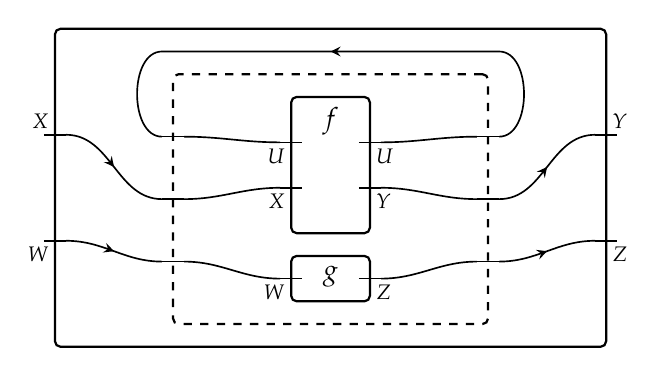
\begin{tikzpicture}[wiring diagram,baseline=(current bounding box.center)]
         \node[bb={2}{2}, bb name=$f$] (X1) {};
         \node[bb port sep=1,bb={1}{1}, below=of X1, bb name=$g$] (X2) {};
         \node[bb={3}{3}, fit={(X1) (X2)}, dashed] (Z) {};
         \node[bb={2}{2}, fit={(Z) ($(Z.north)+(0,1)$)}] (Y) {};
         \draw[ar] (Y_in1') to (Z_in2);
         \draw (Z_in2') to (X1_in2);
         \draw[ar] (Y_in2') to (Z_in3);
         \draw (Z_in3') to (X2_in1);
         \draw (X1_out2) to (Z_out2');
         \draw[ar] (Z_out2) to (Y_out1');
         \draw (X2_out1) to (Z_out3');
         \draw[ar] (Z_out3) to (Y_out2');
         \draw (Z_in1') to (X1_in1);
         \draw (X1_out1) to (Z_out1');
         \draw[ar] let \p1=(Z.north east), \p2=(Z.north west), \n1={\y1+\bby}, \n2=\bbportlen in
             (Z_out1) to[in=0] (\x1+\n2,\n1) -- (\x2-\n2,\n1) to[out=180] (Z_in1);
         \draw[label]
             node[above left=of Y_in1] {$X$}
             node[below left=of Y_in2] {$W$}
             node[above right=of Y_out1] {$Y$}
             node[below right=of Y_out2] {$Z$}
             node[below left=of X1_in1] {$U$}
             node[below left=of X1_in2] {$X$}
             node[below right=of X1_out2] {$Y$}
             node[below right=of X1_out1] {$U$}
             node[below left=of X2_in1] {$W$}
             node[below right=of X2_out1] {$Z$};
      \end{tikzpicture}
      \]
\end{itemize}
For completeness, the rest of the axioms are:
\begin{itemize}
   \item Naturality in $X$: for every $f\colon U\otimes X\to U\otimes Y$ and $g\colon X'\to X$,
      \begin{equation*}
         \Tr^U_{X,Y}[f]\circ g = \Tr^U_{X',Y}\bigl[f\circ(U\otimes g)\bigr]
      \end{equation*}
   \item Naturality in $Y$: for every $f\colon U\otimes X\to U\otimes Y$ and $g\colon Y\to Y'$,
      \begin{equation*}
         g\circ\Tr^U_{X,Y}[f] = \Tr^U_{X,Y'}\bigl[(U\otimes g)\circ f\bigr]
      \end{equation*}
   \item Vanishing 1: for every $f\colon I\otimes X\to I\otimes Y$,
      \begin{equation*}
         \Tr^I_{X,Y}[f] = f
      \end{equation*}
   \item Vanishing 2: for every $f\colon U\otimes V\otimes X\to U\otimes V\otimes Y$,
      \begin{equation*}
         \Tr^{U\otimes V}_{X,Y}[f] = \Tr^U_{X,Y}\bigl[\Tr^U_{V\otimes X,V\otimes Y}[f]\bigr]
      \end{equation*}
   \item Yanking:
      \begin{equation*}
         \Tr^X_{X,X}[\sigma_{X,X}]=X
      \end{equation*}
\end{itemize}

If $\cat{C}$ and $\cat{D}$ are traced categories, then a \emph{(strict) traced functor} is simply a
strict symmetric monoidal functor which preserves the trace operation.

\begin{remark}
      \label{rem:traced_2morphisms}
   Traced categories were first defined in~\cite{JoyalStreetVerity}. However, those authors define
   the 2-morphisms between traced functors to be monoidal transformations, whereas this choice does
   not behave appropriately with their $\Int$ construction (for example $\Int$ would not be
   2-functorial). This error was corrected in \cite{HK}, where it was shown that the appropriate
   2-morphisms between traced functors are natural \emph{isomorphisms}. We denote by $\TTrCat$ the
   corrected 2-category of traced categories (where 2-cells are invertible), and we denote its
   underlying 1-category by $\TrCat$.
\end{remark}

In Remark~\ref{rem:characterization_of_traced} we will be able to formally define the 2-category
$\TTrCat$ without mentioning the $\Tr$ structure or the seven axioms above, but instead via the
relationship between compact and monoidal categories.

\section{Compact categories and the Int construction}
      \label{sec:compact_and_int}

We will denote by $\CCompCat$ the full sub-2-category of $\MMonCat$ spanned by the compact closed
symmetric strict monoidal categories (or just compact categories for short).  Recall that a compact
category is a symmetric monoidal category $(\cat{C},\otimes,I)$ with the property that for every
object $X\in\cat{C}$ there exists an object $X^*$ and morphisms $\eta_X\colon I\to X^*\otimes X$ and
$\epsilon_X\colon X\otimes X^*\to I$ such that the following diagrams commute:
\begin{equation*}
   \begin{tikzcd}[column sep=small]
      X\arrow[r,"\id_X"]\arrow[d,"\cong"'] & X \\
      X\otimes I\arrow[d,"X\otimes\eta_X"'] & I\otimes X\arrow[u,"\cong"'] \\
      X\otimes(X^*\otimes X)\arrow[r,"\cong"'] & (X\otimes X^*)\otimes X\arrow[u,"\epsilon_X\otimes X"']
   \end{tikzcd}
   \hspace{.6in}
   \begin{tikzcd}[column sep=small]
      X^*\arrow[r,"\id_{X^*}"]\arrow[d,"\cong"'] & X^*\\
      I\otimes X^*\arrow[d,"\eta_X\otimes X^*"'] & X^*\otimes I\arrow[u,"\cong"'] \\
      (X^*\otimes X)\otimes X^*\arrow[r,"\cong"'] & X^*\otimes (X\otimes X^*)\arrow[u,"X^*\otimes\epsilon_X"']
   \end{tikzcd}
\end{equation*}
Given a morphism $f\colon X\to Y$ in $\cat{C}$, we denote by $f^*\colon Y^*\to X^*$ the composite
\begin{equation*}
   Y^*\To{\eta_X}X^*\otimes X\otimes Y^* \To{f}X^*\otimes Y\otimes Y^*\To{\epsilon_Y}X^*.
\end{equation*}

It is easy to check that a strong functor $F\colon\cat{C}\to\cat{M}$ preserves all duals that exist
in $\cat{C}$, i.e., there is a natural isomorphism $F(c^*)\iso F(c)^*$. From this, it follows that
if $F,G\colon\cat{C}\to\cat{C'}$ are functors between compact categories, then any natural
transformation $\alpha\colon F\to G$ is a natural isomorphism. Indeed, for any object $c\in\cat{C}$,
the inverse of the $c$-component $\alpha_c\colon Fc\to Gc$ is given by the dual morphism
$(\alpha_{c^*})^*\colon Gc\to Fc$ to the dual component.

Every compact category $\cat{C}$ has a canonical trace structure, defined on a morphism $f\colon
U\otimes X\to U\otimes Y$ morally (up to symmetries and identities) to be $\epsilon_U\circ f\circ
\eta_U$. More precisely, if $\sigma_{A,B}$ is the symmetry isomorphism, one defines
\begin{equation*}
   \Tr^U_{X,Y}[f]\coloneqq(\epsilon_U\otimes Y)\circ (\sigma_{U^*,U}\otimes Y)\circ (U^*\otimes f)\circ (\eta_U\otimes X)
\end{equation*}
Thus we have a functor $\UCT\colon\CCompCat\to\TTrCat$. It is shown
in~\cite{JoyalStreetVerity}~and~\cite{HK} that this functor is the right half of a 2-adjunction
\begin{equation}
      \label{dia:traced_compact_adjunction}
   \begin{tikzcd}
      \TTrCat\arrow[r,shift left=.5ex, "\Int"]&\CCompCat\arrow[l,shift left=.5ex,"\UCT"]
   \end{tikzcd}
\end{equation}
the left half of which we now describe on the level of objects $\cat{M}\in\TTrCat$.

For a traced category $\cat{M}$, let $\widetilde{\cat{M}}$ denote the category with objects given by
pairs $(\inp{X},\outp{X})$ where $\inp{X},\outp{X}\in(\cat{M})$ and morphisms given by
\begin{equation*}
   \Hom_{\widetilde{\cat{M}}}\big((\inp{X},\outp{X}),(\inp{Y},\outp{Y})\big)
      = \Hom_{\cat{M}}(\inp{X}\otimes \outp{Y},\outp{X}\otimes \inp{Y}).
\end{equation*}
For morphisms $\Phi:(\inp{X},\outp{X})\to(\inp{Y},\outp{Y})$ and
$\Psi:(\inp{Y},\outp{Y})\to(\inp{Z},\outp{Z})$ in $\widetilde{\cat{M}}$ we define their composition
to be
\begin{equation*}
   \Psi\circ\Phi\coloneqq\Tr^{\outp{Y}}_{\inp{X}\otimes \outp{Z},\outp{X}\otimes \inp{Z}}\Big[\big(\sigma_{\outp{X},\outp{Y}}\otimes \inp{Z}\big)\circ\big(\outp{X}\otimes\Psi\big)\circ\big(\Phi\otimes \outp{Z}\big)\circ\big(\sigma_{\outp{Y},\inp{X}}\otimes \outp{Z}\big)\Big].
\end{equation*}
It is shown in~\cite{JoyalStreetVerity} that $\Int(\cat{M})\coloneqq\widetilde{\cat{M}}$ is a
compact category whose tensor is given by
\begin{equation*}
   (\inp{X},\outp{X})\odot(\inp{Y},\outp{Y})\coloneqq(\inp{X}\otimes \inp{Y},\outp{X}\otimes \outp{Y})
\end{equation*}
with unit object $\tilde I\coloneqq(I,I)$ and duality
${(\inp{X},\outp{X})}^*\coloneqq(\outp{X},\inp{X})$.

\begin{lemma}
      \label{lemma:fully_faithful_and_trace}
   The following facts hold for any traced category $\cat{C}$:
   \begin{enumerate}[label={\upshape\roman*}.]
      \item The component $\cat{C}\to\Int(\cat{C})$ of the unit of the adjunction
         \eqref{dia:traced_compact_adjunction} is fully faithful. It follows that
         $\Int\colon\TTrCat\to\CCompCat$ is locally fully faithful.
      \item If $\cat{D}$ is a monoidal category and $F\colon\cat{D}\to\cat{C}$ is a fully faithful
         symmetric monoidal functor, then $\cat{D}$ has a unique trace for which $F$ is a traced
         functor.
      \item If $\cat{C}$ is compact then the unit
         $\cat{C}\To{\raisebox{-1ex}{$\equiv$}}\Int(\cat{C})$ is an equivalence.
      \item Suppose that $\cat{C'}$ is a traced category and that $F\colon \cat{C}\to \cat{C}'$ is a
         traced functor. Then $F$ is bijective-on-objects (resp.\ fully faithful) if and only if
         $\Int(F)$ is.
   \end{enumerate}
\end{lemma}
\begin{proof}
   These are all shown in, or trivially derived from,~\cite{JoyalStreetVerity}.
\end{proof}

\section{Free traced and compact categories}
      \label{sec:free_and_geometry}

Let $\CCat$ (resp.\ $\CCat_{\iso}$) denote the 2-category of small categories, functors, and natural
transformations (resp.\ natural isomorphisms). There are free/forgetful (strict) 2-adjunctions of
2-categories, as to the left:
\begin{align}
   \nonumber
   \FM&\colon\CCat_{\;\;} \leftrightarrows\MMonCat:\!\UM
      & \Set &\leftrightarrows\MonCat \\
   \label{eqn:adjunctions}
   \FT&\colon\CCat_{\iso}\leftrightarrows\TTrCat:\!\UT
      & \Set &\leftrightarrows\TrCat \\
   \nonumber
   \FC&\colon\CCat_{\iso}\leftrightarrows\CCompCat:\!\UC
      & \Set&\leftrightarrows\CompCat
\end{align}
These have underlying 1-adjunctions (e.g., $\Cat\leftrightarrows\TrCat$), which \cite{Abramsky2}
constructs in detail. We will not need the 2-adjunctions in the main body of this paper; however,
we prove they exist in Corollary~\ref{cor:2_adjunctions_MonTrComp}. For the time being, we
consider only their underlying 1-adjunctions, which we can compose with the discrete adjunction
$\Disc\colon\Set\leftrightarrows\Cat:\!\Ob$ to obtain 1-adjunctions as to the right in
\eqref{eqn:adjunctions}. We will write $\TM, \TT$, and $\TC$ for the respective monads induced
on $\Set$. Note that $\TM$ and $\TT$ are both isomorphic to the free monoid monad, while $\TC$ is
isomorphic to the free monoid-with-involution monad.%
\footnote{
   Note that $\TM$ is not the free-\emph{commutative}-monoid monad, even though the objects of
   $\MonCat$ are \emph{symmetric} monoidal categories, because the symmetries are encoded in natural
   isomorphisms, not equalities.
}
There is an isomorphism of categories $\Set_{\TM}\iso\Set_{\TT}$, because $\TM\iso\TT$. The Kleisli
categories $\Set_{\TM}$, $\Set_{\TT}$, and $\Set_{\TC}$ are equivalent to the full subcategories of
$\MonCat$, $\TrCat$, and $\CompCat$ (respectively) spanned by objects which are free on a set.

The forgetful functors between the categories of structured monoidal categories commute with the
underlying set functors, i.e.,~the following diagram commutes:
\begin{equation}
   \label{eqn:tetrahedron}
   \begin{tikzcd}
      & \TrCat \ar[dr,"\UTM"] \ar[dd,"\UT" near start] & \\
      \CompCat \ar[rr,crossing over,"\UCM"' near start] \ar[dr,"\UC"'] \ar[ru,"\UCT"]
         && \MonCat \ar[dl,"\UM"] \\
      & \Set &
   \end{tikzcd}
\end{equation}
Because the functor $\UCM\colon\CompCat\to\MonCat$ commutes with the right adjoints of the
adjunctions to $\Set$, i.e., $\UM\UCM=\UC$, it induces a monad morphism $\alpha\colon\TC\to\TM$
(i.e. a natural transformation $\alpha\colon\TM\to\TC$ compatible with the units and
multiplications), given by the composition of the natural transformations
\begin{equation*} \begin{tikzcd}[column sep=2cm]
   \TM\ar[r,equal]\ar[d,dashed,"\alpha"']&\UM\FM\ar[r,"\UM\FM\eta_C"]&\UM\FM\UC\FC\ar[d,equal]\\
   \TC&\UM\UCM\FC\ar[l,equal]&\UM\FM\UM\UCM\FC\ar[l,"\UM\epsilon_M\UCM\FC"]
\end{tikzcd} \end{equation*}
The component $\alpha_{\LabSet}$ of this transformation is simply the evident inclusion of the free
monoid on a set $\LabSet$ into the free monoid-with-involution on $\LabSet$. In this way, $\UCM$
induces a functor between the Kleisli categories in the other direction:
\begin{equation}
      \label{eqn:FMC}
   \FMC\colon\Set_{\TM}\to\Set_{\TC}
\end{equation}

\subsection{$\LCob{\LabSet}$ is the free compact category on $\LabSet$}

To connect the geometry (string diagrams) with the algebra (free compact categories), we recall the
following folklore theorem.

\begin{theorem}
   The free compact category on one generator is equivalent to $\Cob$, the category of oriented
   1-dimensional cobordisms.
\end{theorem}

See \cite[Theorem 3.6]{FreydYetter} for a proof of the non-symmetric version, \cite{Kock} and
\cite{BaezDolan} for the 2-dimensional version with brief comments on the 1-dimensional version. See
also \cite{KellyLaplaza} and \cite{Abramsky2} for combinatorial descriptions of $\Cob$ as the free
compact category functor.  Because the free functor is a left adjoint, hence preserves colimits, we
have the following corollary.

\begin{corollary}
      \label{cor:free_compact_is_Cob}
   For any set $\LabSet$, the free compact category on $\LabSet$ is equivalent to $\LCob{O}$, the
   category of oriented $\LabSet$-labeled 1-cobordisms.
\end{corollary}

\subsection{Set-theoretic description of $\Cob$}

Here we give a brief combinatorial description of the category $\Cob$, for the reader's convenience.
The objects are finite signed sets, $X=(\inp{X},\outp{X})$. A morphism $X\to Y$ can be identified
with a set $C$ and four injections (left-hand side of \eqref{eqn:describing_cob}):
\begin{equation}
      \label{eqn:describing_cob}
\begin{tikzcd}[row sep=1cm, column sep = 1cm]
   &\inp{X}\ar[d]\\
   \outp{X}\ar[r]&C&\inp{Y}\ar[l]\\
   &\outp{Y}\ar[u]
\end{tikzcd}
\hspace{.6in}
\begin{tikzcd}[row sep=.5cm, column sep =.5cm]
   &\inp{X}\ar[d]\\
   \outp{X}\ar[r]&C&\inp{Y}\ar[l]\ar[d]\\
   &\outp{Y}\ar[u]\ar[r]&D&\inp{Z}\ar[l]\\
   &&\outp{Z}\ar[u]
\end{tikzcd}
\end{equation}
such that the image of the vertical maps $\inp{X}+\outp{Y}\to C$ is equal to that of the horizontal
maps, $\outp{X}+\inp{Y}\to C$. Composition is achieved by quotienting the middle square in the
right-hand diagram of \eqref{eqn:describing_cob}, while the monoidal structure is provided by
disjoint unions of sets.

\section{Orthogonal factorization systems}
      \label{sec:factorization_systems}

We use orthogonal factorization systems throughout this paper, mainly to deal with the issue of
object-variance, mentioned in Section~\ref{subsec:main_results}. Background on orthogonal
factorization systems can be found in \cite[Chapter 5.5]{BorceuxV1}. Here we describe the
$\cat{V}$-enriched notion, for two cases, the usual 1-categorical case, where $\cat{V}=\Set$, and
the strict 2-categorical case, where $\cat{V}=\Cat$.

\begin{definition}
      \label{def:orthogonal}
   Let $\cat{V}$ be either $\Set$ or $\Cat$, and suppose that $\cat{C}$ is a $\cat{V}$-enriched
   category. An \emph{orthogonal factorization system in $\cat{C}$} consists of two distinguished
   classes of morphisms, $(\cat{L},\cat{R})$, with the following properties:
   \begin{itemize}
      \item Each morphism $f\in\cat{C}$ factors as $f=e\circ m$, where $m\in\cat{L}$ and
         $e\in\cat{R}$.
      \item If $m\colon a\to b$ in $\cat{L}$ and $e\colon c\to d$ in $\cat{R}$, then the left-hand
         square below is a pullback in $\cat{V}$:
         \begin{equation}
               \label{eqn:OrthFactSys}
            \begin{tikzcd}
               \cat{C}(b,c)\ar[r]\ar[d]\ar[rd,phantom,"\lrcorner" very near start]&\cat{C}(a,c)\ar[d,"e\circ -"]\\
               \cat{C}(b,d)\ar[r,"-\circ m"']&\cat{C}(a,d)
            \end{tikzcd}
            \hspace{.9in}
            \begin{tikzcd}
               a\ar[r,"\forall"]\ar[d,two heads,"m"']&c\ar[d,hook, "e"]\\
               b\ar[r,"\forall"']\ar[ur,dashed,"\exists!"]&d
            \end{tikzcd}
         \end{equation}
         In particular, for all solid arrow squares, as in the right-hand diagram, there exists a
         unique diagonal filler. We say that $m$ is ``left-orthogonal'' to $e$, or that $e$ is
         ``right-orthogonal'' to $m$, and denote this relation as $m\boxslash e$.
      \item If $m\boxslash e$ for all $e\in\cat{R}$, then $m\in\cat{L}$. Likewise, if $m\boxslash e$
         for all $m\in\cat{L}$, then $e\in\cat{R}$.
   \end{itemize}
   As shown, we often indicate morphisms in $\cat{L}$ using a two-headed arrow and morphisms in
   $\cat{R}$ using a hooked arrow.
\end{definition}

The case of bijective-on-objects / fully faithful factorization systems on certain 2-categories
($\Cat$-enriched categories) will be useful throughout the paper.

\begin{definition}
      \label{def:fully_faithful}
   Say that a morphism $f\colon a\to b$ in a 2-category $\ccat{C}$ is \emph{fully faithful} if the
   functor $\ccat{C}(x,a)\to\ccat{C}(x,b)$, induced by composition with $f$, is fully faithful for
   every $x$.

   That is, $f$ is fully faithful if, for every diagram
   \begin{equation*} \begin{tikzcd}[row sep=large]
         x \ar[r,bend left,"u"] \ar[r,bend right,"v"']
               \ar[d,equal]
            & a \ar[d,"f"] \\
         x \ar[r,bend left,"u'" domA] \ar[r,bend right,"v'"' codA]
            & b
         \twocellA{\alpha'}
   \end{tikzcd} \end{equation*}
   such that $fu=u'$ and $fv=v'$, there exists a unique $\alpha\colon u\Rightarrow v$ such that
   $f\alpha=\alpha'$.
\end{definition}

\begin{definition}
      \label{def:bijective_on_objects}
   Say that a morphism $f\colon a\to b$ in a 2-category $\ccat{C}$ is \emph{bijective-on-objects} if
   it is left orthogonal to every fully faithful morphism.

   We say that a 2-category \emph{has a bijective-on-objects / fully faithful factorization system}
   if these two classes form an orthogonal factorization system as in
   Definition~\ref{def:orthogonal}.
\end{definition}

\chapter{Background on equipments}
      \label{chap:background_equipments}

This section introduces equipments, which we use to properly situate traced and compact categories.
This tool will eventually allow us to clarify the relationship between strict monoidal functors
between monoidal categories and lax monoidal functors to $\Set$.

\section{Profunctors}
      \label{sec:profunctors}
Let $\cat{C}$ and $\cat{D}$ be categories. Recall that a profunctor $M$ from $\cat{C}$ to $\cat{D}$,
written
\[ \begin{tikzcd}
   \cat{C} \ar[r,tick,"M"] & \cat{D},
\end{tikzcd} \]
is defined to be a functor $M\colon\op{\cat{C}}\times\cat{D}\to\Set$. We can think of a profunctor
as a sort of graded bimodule: for each object $c\in\cat{C}$ and $d\in\cat{D}$ there is a set
$M(c,d)$ of elements in the bimodule, and given an element $m\in M(c,d)$ and morphisms $f\colon
c'\to c$ in $\cat{C}$ and $g\colon d\to d'$ in $\cat{D}$, there are elements $g\cdot m\in M(c,d')$
and $m\cdot f\in F(c',d)$, such that the equations $(g\cdot m)\cdot f=g\cdot(m\cdot f)$,
$g'\cdot(g\cdot m)=(g'\circ g)\cdot m$, and $(m\cdot f)\cdot f'=m\cdot(f\circ f')$ hold whenever
they make sense.

If $F\colon\cat{C}'\to\cat{C}$ and $G\colon\cat{D}'\to\cat{D}$ are functors, and $M$ is a profunctor
as before, then there is a profunctor $M(F,G)$ from $\cat{C}'$ to $\cat{D}'$, defined to be the
composite
\[ \begin{tikzcd}
   \op{\cat{C}'}\times\cat{D}' \ar[r,"\op{F}\times G"]
      &[1.5em] \op{\cat{C}}\times\cat{D} \ar[r,"M"]
      & \Set.
\end{tikzcd} \]
In other words, for any objects $c\in\cat{C}'$ and $d\in\cat{D}'$, the profunctor $M(F,G)$ has
elements $M(Fc,Gd)$, and if $m\in M(Fc,Gd)$ and $g\colon d\to d'$ is a morphism in $\cat{D}'$, then
the element $m\cdot g$ in $M(F,G)$ is defined by the element $m\cdot G(g)$ in $M$, and similarly for
the $\cat{C}'$ action.

Given two profunctors
\[ \begin{tikzcd}
   \cat{C} \ar[r,tick,shift left,"M"] \ar[r,tick,shift right,"N"'] & \cat{D}
\end{tikzcd} \]
define a profunctor morphism $\phi\colon M\Rightarrow N$ to be a natural transformation. In other
words, for each $c\in\cat{C}$ and $d\in\cat{D}$ there is a function $\phi_{c,d}\colon M(c,d)\to
N(c,d)$ such that the equation $\phi(f\cdot m \cdot g)=f\cdot\phi(m)\cdot g$ holds whenever it makes
sense.

There is a tensor product of profunctors: given two profunctors
\[ \begin{tikzcd}
   \cat{C} \ar[r,tick,"M"] & \cat{D} \ar[r,tick,"N"] & \cat{E}
\end{tikzcd} \]
define the profunctor $M\otimes N$ such that for objects $c\in\cat{C}$ and $e\in\cat{E}$, $(M\otimes
N)(c,e)$ is the coequalizer of the diagram
\begin{equation} \begin{tikzcd}
   \label{eqn:coendComp}
   \displaystyle\coprod_{d_1,d_2\in\cat{D}} M(c,d_1)\times\cat{D}(d_1,d_2)\times N(d_2,e)
      \ar[r,shift left] \ar[r,shift right]
   & \displaystyle\coprod_{d\in\cat{D}} M(c,d)\times N(d,e)
\end{tikzcd} \end{equation}
where the two maps are given by the right action of $\cat{D}$ on $M$ and by the left action of
$\cat{D}$ on $N$. We can write elements of $(M\otimes N)(c,e)$ as tensors $m\otimes n$, where $m\in
M(c,d)$ and $n\in N(d,e)$ for some $d\in\cat{D}$. The coequalizer then implies that $(m\cdot
f)\otimes n=m\otimes(f\cdot n)$ whenever the equation makes sense.

For any category $\cat{C}$, there is a profunctor
$\Hom_{\cat{C}}\colon\op{\cat{C}}\times\cat{C}\to\Set$, and these hom profunctors act as units for
the tensor product. More precisely, if $M$ is as above, there are canonical isomorphisms
$\Hom_{\cat{C}}\otimes M \iso M \iso M\otimes\Hom_{\cat{D}}$.

\section{Equipments}

A double category is a 2-category-like structure involving horizontal and vertical arrows, as well
as 2-cells. An equipment (sometimes called a \emph{proarrow equipment} or \emph{framed bicategory})
is a double category satisfying a certain fibrancy condition. In this section, we will spell this
out and give a few examples. An excellent reference is Shulman's paper \cite{Shulman}; see also
\cite{Wood1} and \cite{Wood2}.

\begin{definition}
   A \emph{double category} $\dcat{D}$ consists of the following data:
   \begin{itemize}
      \item A category $\dcat{D}_0$, which we refer to as the \emph{vertical category} of
         $\dcat{D}$. For any two objects $c,d\in\dcat{D}_0$, we will write
         $\dcat{D}_0(c,d)$ for the set of vertical arrows from $c$ to $d$. We refer to
         objects of $\dcat{D}_0$ as objects of $\dcat{D}$.
      \item A category $\dcat{D}_1$, equipped with two functors $L,R\colon\dcat{D}_1\to\dcat{D}_0$,
         called the \emph{left frame} and \emph{right frame} functors. Given an object
         $A\in\Ob\dcat{D}_1$ with $c=L(A)$ and $c'=R(A)$, we say that $A$ is a \emph{proarrow} (or
            \emph{horizontal arrow}) \emph{from $c$ to $c'$} and write $A\colon c\tickar c'$. A
            morphism $\phi\colon A\to B$ in $\dcat{D}_1$ is called a 2-cell, and is drawn as
            follows, where $f=L(\phi)$ and $f'=R(\phi)$:
         \begin{equation} \begin{tikzcd}
               \label{eqn:2cell}
            c \ar[r,tick,"A" domA] \ar[d,"f"']
            & c'\ar[d,"{f'}"]
              \\
            d \ar[r,tick,"B"' codA]
              & d'
            \twocellA{\phi}
         \end{tikzcd} \end{equation}
      \item A \emph{unit} functor $U\colon\dcat{D}_0\to\dcat{D}_1$, which is a
         section of both $L$ and $R$, i.e., $L\circ U=\id_{\dcat{D}_0}=R\circ U$. We will often
         abuse notation by writing $c$ for the unit proarrow $U(c)\colon c\tickar c$, and similarly
         for vertical arrows.
      \item A functor $\odot\colon\dcat{D}_1\times_{\dcat{D}_0}\dcat{D}_1\to\dcat{D}_1$, called
         \emph{horizontal composition}, that is weakly associative and unital in the sense that
         there are coherent unitor and associator isomorphisms. See \cite{Shulman} for details.
   \end{itemize}
   Given a double category $\dcat{D}$ there is a strict 2-category called the \emph{vertical
   2-category}, denoted $\VVer(\dcat{D})$, whose underlying 1-category is $\dcat{D}_0$, and whose
   2-morphisms $f\Rightarrow f'$ are defined to be 2-cells \eqref{eqn:2cell} where $c'=c$, $d'=d$,
   and $A$ and $B$ are unit proarrows. There is also a \emph{horizontal bicategory}, denoted
   $\HHor(\dcat{D})$, whose objects and 1-cells are the objects and horizontal 1-cells of
   $\dcat{D}$, and whose 2-cells are the 2-cells of $\dcat{D}$ of the form \eqref{eqn:2cell} such
   that $f=\id_c$ and $f'=\id_{c'}$.

   A \emph{strong double functor} $\dcat{C}\to\dcat{D}$ consists of functors
   $\dcat{C}_0\to\dcat{D}_0$ and $\dcat{C}_1\to\dcat{D}_1$ commuting with the frames $L,R$, and
   preserving the unit $U$ and horizontal composition $\odot$ up to coherent isomorphism.
\end{definition}

\begin{definition}
      \label{def:equipment}
   An \emph{equipment} is a double category $\dcat{D}$ in which the frame functor
   \[
      (L,R)\colon\dcat{D}_1\onto\dcat{D}_0\times\dcat{D}_0
   \]
   is a fibration. If $f\colon c\to c'$ and $g\colon d\to d'$ are vertical morphisms and $B\colon
   c'\tickar d'$ is a proarrow, a cartesian morphism $A\to B$ in $\dcat{D}_1$ over $(f,g)$ is a
   2-cell
   \[ \begin{tikzcd}
      c \ar[r,tick, "A" domA] \ar[d,"f"']
         & d\ar[d,"{g}"] \\
      c' \ar[r,tick,"B"' codA]
         & d'
      \twocellA{\tn{cart}}
   \end{tikzcd} \]
   which we call a \emph{cartesian 2-cell}. We refer to $A$ as the \emph{restriction of $B$ along
   $f$ and $g$}, written $A=B(g,f)$.

   By an \emph{equipment functor}, we simply mean a strong double functor between equipments.
\end{definition}

\begin{example}
   An equipment $\dcat{D}$ is often named according to its horizontal arrows. In
   Section~\ref{sec:profunctors} we discussed profunctors, which are the horizontal arrows in an
   equipment $\dProf$. Variations on $\dProf$, such as $\dMonProf, \dTrProf,$ and $\dCompProf$
   (defined in Section~\ref{sec:monoidal_profunctors}) will play a major role in this paper.

   The vertical category of $\dProf$ is the 1-category $\dProf_0=\Cat$ of small 1-categories and
   functors. Given objects $C,D\in\dProf_0$, a horizontal arrow between them is a profunctor
   $C\tickar D$, as described in Section~\ref{sec:profunctors}. A 2-cell $\phi$ in $\dProf$, as to
   the left, denotes a natural transformation, as to the right, in \eqref{eqn:Prof2cells}:
   \begin{equation}
         \label{eqn:Prof2cells}
      \begin{tikzcd}
         A \ar[r,tick,"X" domA] \ar[d,"F"']
            & B\ar[d,"{G}"] \\
         C \ar[r,tick,"Y"' codA]
            & D
         \twocellA{\phi}
      \end{tikzcd}
      \hspace{.6in}
      \begin{tikzcd}[column sep=.8em, row sep=5ex]
         \op{A}\times B \ar[dr,"X"'] \ar[rr,"\op{F}\times G"]
            & \ar[d,phantom,"\overset{\phi}{\Rightarrow}" near start]
            & \op{C}\times D\ar[dl,"Y"] \\
         & \Set
      \end{tikzcd}
   \end{equation}
   The horizontal composite of profunctors is defined by the coequalizer \eqref{eqn:coendComp}. Note
   that the coequalizer \eqref{eqn:coendComp} is in fact a reflexive coequalizer, using $\id_b\in
   B(b,b)$.

   One can show that the we have defined a double category, and it is an equipment because for any
   $F, G,Y$ as in \eqref{eqn:Prof2cells}, there is a cartesian 2-cell whose domain is the profunctor
   $X\coloneqq Y\circ(\op{F}\times G)$ obtained by composition.

   It follows (by an easy Yoneda lemma argument) that $\VVer(\dProf)\equiv\CCat$, the 2-category of
   small categories.
\end{example}

\begin{example}
      \label{ex:dspan}
   There is an equipment $\dSpan$ of spans in $\Set$. Its vertical category is
   $\dSpan_0\coloneqq\Set$. A horizontal 1-cell between sets $A$ and $B$ is a span $A\from S\to B$,
   their composition is defined by a pullback of spans, and a 2-cell in $\dSpan$ is a commutative
   diagram in $\Set$ of the obvious shape. A cartesian 2-cell in this equipment is obtained by
   taking an evident limit in $\Set$.
\end{example}

\begin{definition}
      \label{def:local_equivalence}
   We refer to an equipment functor $F\colon\dcat{C}\to\dcat{D}$ as a \emph{local equivalence} if
   the following square is a pseudo-pullback of categories:
   \begin{equation} \begin{tikzcd}
         \label{eqn:local_equiv}
      \dcat{C}_1 \ar[r,"F_1"] \ar[d,two heads] \ar[dr,phantom,"\lrcorner" very near start]
         & \dcat{D}_1 \ar[d,two heads] \\
      \dcat{C}_0\times\dcat{C}_0 \ar[r,"F_0\times F_0"']
         & \dcat{D}_0\times\dcat{D}_0
   \end{tikzcd} \end{equation}
   where the left-hand and right-hand arrows are the frame fibrations.

   If moreover $F_0\colon\dcat{C}_0\to\dcat{D}_0$ is fully faithful, we say that $F$ is a
   \emph{fully faithful local equivalence}.
\end{definition}

\begin{remark}
      \label{rem:strict_vs_pseudo_pullback}
   It is a standard fact that, for 1-categories, a strict pullback of an isofibration along an arbitrary
   functor is also a pseudo-pullback. Any Grothendieck fibration (or opfibration) is in
   particular an isofibration, so if the square \eqref{eqn:local_equiv} is a strict pullback, then it
   is also a pseudo-pullback.
\end{remark}

\begin{definition}
      \label{def:induced_locally_equivalent_equipment}
   Let $\dcat{D}$ be a double category and $F_0\colon\dcat{C}_0\to\dcat{D}_0$ be a functor. A strict
   pullback of the form \eqref{eqn:local_equiv} defines a double category $\dcat{C}$, which we denote
   \[
      \dcat{C}\coloneqq F_0^*(\dcat{D})
   \]
   and call the \emph{equipment induced by $F_0$}. If $\dcat{D}$ is an equipment, $F_0^*(\dcat{D})$
   will be as well, because fibrations are stable under pullback. By
   Remark~\ref{rem:strict_vs_pseudo_pullback}, the induced equipment functor
   $F_0^*(\dcat{D})\to\dcat{D}$ is a local equivalence.
\end{definition}

\section{The monoids and bimodules construction}
      \label{sec:monoids_bimods}

\begin{definition}
      \label{def:monoids_and_modules}
   Let $\dcat{D}$ be an equipment with local coequalizers, i.e.,~such that each category
   $\HHor(\dcat{D})(A,B)$ has coequalizers and $\odot$ preserves coequalizers in each variable. The
   equipment $\dMod(\dcat{D})$ of \emph{monoids and bimodules} is defined as follows (see also
   \cite{Shulman}):
   \begin{itemize}
      \item The vertical category $\dMod(\dcat{D})_0$, denoted $\Mon(\dcat{D})$, is the category of monoids in $\dcat{D}$.  More precisely, the objects are \emph{monoids}: tuples $(c,M,i_M,m_M)$ consisting of an
         object $c$ of $\dcat{D}$ and a proarrow $M\colon c\tickar c$ together with unit and
         multiplication cells
         \begin{equation}
               \label{eqn:unit_and_mult}
            \begin{tikzcd}
               c \ar[r,tick,"c" domA] \ar[d,equal]
                  & c \ar[d,equal] \\
               c \ar[r,tick,"M"' codA] & c
               \twocellA{i_M}
            \end{tikzcd}
            \qquad
            \begin{tikzcd}
              c \ar[r,tick,"M"] \ar[d,equal]
                 & |[alias=domA]| c \ar[r,tick,"M"]
                 & c \ar[d,equal] \\
              c \ar[rr,tick,"M"' codA]
                 && c
              \twocellA{m_M}
            \end{tikzcd}
         \end{equation}
         satisfying the evident unit and associativity axioms.  The vertical arrows are \emph{monoid homomorphisms}: pairs $(f,\vec{f}\mspace{2mu})$ consisting of a vertical arrow
         $f\colon c\to d$ in $\dcat{D}$ and a cell
         \[ \begin{tikzcd}
            c \ar[r,tick,"M" domA] \ar[d,"f"']
               & c \ar[d,"f"] \\
            d \ar[r,tick,"N"' codA]
               & d
            \twocellA{\vec{f}}
         \end{tikzcd} \]
         which respects the unit and multiplication cells of $M$ and $N$.
      \item The proarrows $B\colon M\tickar N$ are \emph{bimodules}: triples $(B,l_B,r_B)$
         consisting of a proarrow $B\colon c\tickar d$ in $\dcat{D}$ and cells
         \begin{equation*}
            \begin{tikzcd}
               c \ar[r,tick,"M"] \ar[d,equal]
                  & |[alias=domA]| c \ar[r,tick,"B"]
                  & d \ar[d,equal] \\
               c \ar[rr,"B"' codA]
                  && d
               \twocellA{l_B}
            \end{tikzcd}
            \qquad
            \begin{tikzcd}
               c \ar[r,tick,"B"] \ar[d,equal]
                  & |[alias=domA]| d \ar[r,tick,"N"]
                  & d \ar[d,equal] \\
               c \ar[rr,"B"' codA]
               && d
               \twocellA{r_B}
            \end{tikzcd}
         \end{equation*}
         satisfying evident monoid action axioms.
      \item The horizontal composition $B_1\otimes B_2$ of bimodules $B_1\colon M\tickar M'$ and
         $B_2\colon M'\tickar M''$ is given by the coequalizer in $\HHor(\dcat{D})(M,M'')$
         \[
            B_1\odot M'\odot B_2 \rightrightarrows B_1\odot B_2 \to B_1\otimes B_2
         \]
         together with the evident left $M$ and right $M''$ actions.
      \item The 2-cells are \emph{bimodule homomorphisms}: cells in $\dcat{D}$
         \[ \begin{tikzcd}
           c \ar[r,tick,"A"] \ar[d,"f"' domA]
              & d \ar[d,"g" codA] \\
           c' \ar[r,tick,"B"']
              & d'
           \twocellA{\phi}
         \end{tikzcd} \]
         which are compatible with the left and right actions of the bimodules.
   \end{itemize}
\end{definition}

If $F\colon\dcat{C}\to\dcat{D}$ is an equipment functor, then there is an evident equipment
functor $\dMod(F)\colon\dMod(\dcat{C})\to\dMod(\dcat{D})$.  In fact, we have the following which is immediate from the definitions.
\begin{lemma}
      \label{lemma:FFLE_Mod}
   Let $F\colon\dcat{C}\to\dcat{D}$ be an equipment functor. If $F$ is a local equivalence then so is $\dMod(F)\colon\dMod(\dcat{C})\to\dMod(\dcat{D})$.  If, moreover, $F$ is fully faithful then so is $\dMod(F)$.
\end{lemma}


\begin{example}
      \label{ex:monoid_in_Prof}
   Consider a monoid $M\colon C\tickar C$ in $\dProf$. The unit is a profunctor morphism
   $i\colon\Hom_{C}\to M$. So for any $g\colon c\to d$ in $C$ there is an element $i(g)\in M(c,d)$,
   such that
   \begin{equation}
         \label{eq:Prof_monoid_unit}
      f\cdot i(g)\cdot h = i(f\circ g\circ h)
   \end{equation}
   whenever this makes sense.

   The multiplication $M\odot M\to M$ is an operation assigning to any elements $m_1\in M(c,d)$ and
   $m_2\in M(d,e)$ an element $m_2\bullet m_1\in M(c,e)$, which is associative and satisfies the
   following equations whenever they make sense:
   \begin{gather}
      (f\cdot m_2)\bullet(m_1\cdot h) = f\cdot(m_2\bullet m_1)\cdot h
         \label{eq:Prof_monoid_A}
      \\ (m_3\cdot g)\bullet m_1 = m_3\bullet(g\cdot m_1)
         \label{eq:Prof_monoid_B}
      \\ m\bullet i(f) = m\cdot f
            \quad\text{and}\quad
         i(g)\bullet m = g\cdot m
         \label{eq:Prof_monoid_C}
   \end{gather}
   Specifically, equations \eqref{eq:Prof_monoid_A} and \eqref{eq:Prof_monoid_B} simply say that
   $\bullet$ is a well defined morphism $M\odot M\to M$, while \eqref{eq:Prof_monoid_C} says that
   $\bullet$ is unital with respect to $i$.
\end{example}

\begin{remark}
      \label{rem:suffices_for_monoid}
   It is easy to see that equations \eqref{eq:Prof_monoid_A} and \eqref{eq:Prof_monoid_B} follow
   from \eqref{eq:Prof_monoid_C} and the associativity of $\bullet$. Thus, when proving that
   $\bullet\colon M\odot M\to M$ and $i\colon\Hom_C\to M$ form a monoid, it suffices to prove
   \eqref{eq:Prof_monoid_unit}, \eqref{eq:Prof_monoid_C}, and associativity of $\bullet$.
\end{remark}

\begin{example}
      \label{ex:mod_span_prof}
   Let $\dSpan$ be the equipment defined in Example~\ref{ex:dspan}. A monoid in $\dSpan$ consists of
   a set $C$ and a span $C\from S\to C$, together with a function $e\colon C\to S$ and a function
   $m\colon S\times_C S\to S$, satisfying certain properties. This is precisely the data required to
   define a small category, whose object set is $C$ and morphism set is $S$, with identities given
   by $e$ and composition given by $m$. Similarly, one can identify monoid homomorphisms in $\dSpan$
   with functors between categories and bimodules in $\dSpan$ with profunctors between categories.
   In other words, we have $\dMod(\dSpan)\iso\dProf$.
\end{example}

There is an evident forgetful equipment functor $\MOb\colon\dMod(\dcat{D})\to\dcat{D}$ sending a
monoid $M\colon c\tickar c$ to its underlying object $c=|M|$. We denote its vertical part,
$\Mon(\dcat{D})\to\dcat{D}_0$ the same way. There is also an equipment functor
$U\colon\dcat{D}\to\dMod(\dcat{D})$, sending $d$ to the unit $d\tickar d$ with the trivial monoid
structure, which is a local equivalence.

\begin{lemma}
   Let $\dcat{D}$ be an equipment, $f\colon c\to d$ a vertical morphism, and $N\colon d\tickar d$ a
   monoid. There is a unique monoid structure on the restriction $N(f,f)$ such that the cartesian
   2-cell is a monoid homomorphism. In other words, $\MOb\colon\Mon(\dcat{D})\to\dcat{D}_0$ is a
   fibration, and there is a morphism of fibrations
   \[ \begin{tikzcd}[column sep=tiny]
      \Mon(\dcat{D}) \ar[d,two heads,"\MOb"'] \ar[r]
         & \dcat{D}_1 \ar[d,two heads] \\
      \dcat{D}_0 \ar[r,"\Delta"']&\dcat{D}_0\times\dcat{D}_0.
   \end{tikzcd} \]
\end{lemma}

\begin{definition}
      \label{def:ptd}
   Let $\dcat{D}$ be an equipment. There is a fibration
   $\Ptd(\dcat{D})\twoheadrightarrow\dcat{D}_0$, whose objects are ``pointed proarrows''---proarrows
   $A\colon d\tickar d$ in $\dcat{D}$ equipped with a unit from \eqref{eqn:unit_and_mult}, but not a
   multiplication---and whose morphisms are 2-cells (as in a monoid homomorphism) which preserve the
   units.

   The fibration morphism $\Mon(\dcat{D})\to\dcat{D}_0$ factors through $\Ptd(\dcat{D})$ in the
   evident way. We will not again mention $\Ptd(\dcat{D})$ until Section~\ref{sec:special_CompProf}.
\end{definition}

\begin{lemma}
      \label{lem:Mon_pullback}
   Let $F\colon\dcat{C}\to\dcat{D}$ be a local equivalence. Then the induced square
   \[ \begin{tikzcd}
      \Mon(\dcat{C}) \ar[r,"\Mon(F)"] \ar[d,two heads,"\MOb"'] \ar[dr,phantom,"\lrcorner" very near start]
         & \Mon(\dcat{D}) \ar[d,two heads,"\MOb"] \\
      \dcat{C}_0 \ar[r,"F_0"']
         & \dcat{D}_0
   \end{tikzcd} \]
   is a pseudo-pullback of categories.
\end{lemma}
\begin{proof}
   We may assume without loss of generality that the pullback in Definition~\ref{def:local_equivalence} realizing $F\colon\dcat{C}\to\dcat{D}$ as a local equivalence is strict.  With this simplification, it is then straightforward to check directly that the above square is again a strict pullback, and hence (by Remark~\ref{rem:strict_vs_pseudo_pullback}) is a pseudo-pullback.
\end{proof}

\section{Exactness and the $(\bo,\ff)$ factorization}
      \label{sec:exactness_and_boff}

This section recalls some material from~\cite{Schultz2015} which will be needed in the present
paper. In particular, we recall the definition of an exact equipment in
Definition~\ref{def:exact_equipment}, and the $(\bo,\ff)$ factorization system in
Theorem~\ref{thm:orthogonal}.

\begin{definition}
      \label{def:embedding}
   Let $M\colon c\tickar c$ be a monoid in an equipment $\dcat{D}$. An \emph{embedding} of $M$ into
   an object $x\in\dcat{D}_0$ is a monoid homomorphism $(f,\vec{f}\mspace{2mu})$ from $M$ to the trivial monoid on $x$:
   \[ \begin{tikzcd}
      c \ar[r,tick,"M" domA] \ar[d,"f"']
         & c \ar[d,"f"] \\
      x \ar[r,tick,"x"' codA]
         & x
      \twocellA{\vec{f}}
   \end{tikzcd} \]
   We will sometimes write an embedding as $(f,\vec{f}\mspace{2mu})\colon(c,M)\to x$, or even just $f\colon M\to
   x$ when clear from context. We will write $\Emb(M,x)$ for the set of embeddings from $M$ to $x$.
   This defines a functor $\Emb\colon\op{\Mon(\dcat{D})}\times\dcat{D}_0\to\Set$.
\end{definition}

\begin{lemma}
      \label{lemma:embed_for_LE}
   Suppose that $F\colon\dcat{C}\to\dcat{D}$ is a local equivalence induced by
   $F_0\colon\dcat{C}_0\to\dcat{D}_0$. Suppose $M\in\Mon(\dcat{C})$ is a monoid and $c\in\dcat{C}_0$
   is an object, and let $N=\Mon(F)(M)$ and $d=F_0(c)$. Then we have a pullback square, natural in
   $M$ and $c$:
      \[ \begin{tikzcd}
         \Emb_{\dcat{C}}(M,c)\ar[r]\ar[d]\ar[rd,phantom,"\lrcorner" very near start]
         &\Emb_{\dcat{D}}(N,d)\ar[d]
         \\
         \dcat{C}_0(|M|,c)\ar[r]
         &\dcat{D}_0(|N|,d)
      \end{tikzcd} \]
\end{lemma}

\begin{definition}
   Let $M\colon c\tickar c$ be a monoid in an equipment $\dcat{D}$. The \emph{collapse} of $M$ is defined to be a
   universal embedding of $M$. That is, the collapse of $M$ is an object $\Col{M}\in\dcat{D}_0$ together with an
   embedding
   \[ \begin{tikzcd}
      c \ar[r,tick,"M" domA] \ar[d,"i_M"']
      & c \ar[d,"i_M"]
      \\
      \Col{M} \ar[r,tick,"\Col{M}"' codA]
      & \Col{M}
      \twocellA{\vec{\imath}_M}
   \end{tikzcd} \]
   such that any other embedding of $M$ factors uniquely through $\vec{\imath}_M$:
   \begin{equation*}
      \begin{tikzcd}
         C \ar[r,tick,"M" domA] \ar[d,"f"']
         & C \ar[d,"f"]
         \\
         X \ar[r,tick,"X"']
         & X
         \twocellA{\vec{f}}
      \end{tikzcd}
      \quad = \quad
      \begin{tikzcd}
         C \ar[r,tick,"M" domA] \ar[d,"i_M"']
         & C \ar[d,"i_M"]
         \\
         \Col{M} \ar[r,tick,"\Col{M}"' {domB,codA}] \ar[d,"\tilde{f}"']
         & \Col{M} \ar[d,"\tilde{f}"]
         \\
         X \ar[r,tick,"X"' codB]
         & X
         \twocellA{\vec{\imath}_M}
         \twocellB[pos=.6]{\id_{\tilde{f}}}
      \end{tikzcd}
   \end{equation*}
   In other words, $\Col{M}$ represents the functor $\Emb(M,\textrm{--})\colon\dcat{D}_0\to\Set$.
\end{definition}

We recall the definition of exact equipments from~\cite[Proposition 5.4]{Schultz2015}.  
For monoids $M$ and $N$, we denote by $\Bimod{M}{N}$ the 1-category of $(M,N)$-bimodules and
bimodule morphisms.

\begin{definition}
      \label{def:exact_equipment}
   An equipment $\dcat{D}$ is \emph{exact} if
   \begin{itemize}
      \item every monoid $M\colon c\tickar c$ has a collapse as above, with $\vec{\imath}_M$
         cartesian, and
      \item for every pair of monoids $M$ and $N$ the restriction functor
         \begin{equation}
               \label{eqn:exact_Hor_Bimod}
            \HHor(\dcat{D})(\Col{M},\Col{N})\To{\raisebox{-1ex}{$\equiv$}}\Bimod{M}{N}
         \end{equation}
         is an equivalence of categories.
   \end{itemize}
\end{definition}

It is proven in \cite[Proposition~5.2]{Schultz2015} that for any equipment $\dcat{D}$, its equipment
$\dMod(\dcat{D})$ of monoids and modules is exact. Thus Proposition~\ref{prop:Prof_is_exact} follows
from Example~\ref{ex:mod_span_prof}, but we prove the result directly because it serves as a model
for later exactness proofs.

\begin{proposition}
      \label{prop:Prof_is_exact}
   The equipment $\dProf$ is exact.
\end{proposition}
\begin{proof}
   Let $M\colon C\tickar C$ be a monoid in $\dProf$, as in Example~\ref{ex:monoid_in_Prof}. It is
   straightforward to use $M$ to construct a category $\Col{M}$ with the same objects as $C$, and
   with hom sets defined by $\Col{M}(c,d)\coloneqq M(c,d)$, for any pair of objects $c,d\in\Ob(C)$.
   For any object $c$, the identity is provided by $i(\id_C)$, while the multiplication $\bullet$ of
   $M$ provides the composition of $\Col{M}$.

   The unit of $M$ can also be used to construct an identity-on-objects functor $i_M\colon
   C\to\Col{M}$, and the 2-cell $\vec{\imath}_M$ is trivial, sending any element of $M$ to itself as
   a morphism of $\Col{M}$. It is easy to see that $\vec{\imath}_M$ is cartesian, and that
   $(i_M,\vec{\imath}_M)$ is a collapse. It is also simple to verify the second part of
   Definition~\ref{def:exact_equipment}: a $(M,N)$-bimodule is precisely the data of a profunctor
   $\Col{M}\tickar\Col{N}$.
\end{proof}

\begin{example}
      \label{ex:span_not_exact}
   The equipment $\dSpan$ from Example~\ref{ex:dspan} is not exact. The collapse of a monoid $C\from
   S\to C$ in $\dSpan$ must be its pushout $\Col{S}\iso C\sqcup_SC$, but the associated embedding is
   not cartesian. The second condition of exactness also fails.
\end{example}

\begin{proposition}
      \label{prop:collapse_local_equivalence}
   If $\dcat{D}$ is an exact equipment, then collapse induces an equipment functor denoted
   $\ColDash\colon\dMod(\dcat{D})\to\dcat{D}$. The functor $\ColDash$ is a local equivalence.
\end{proposition}
\begin{proof}
   It is easy to use the universal property of collapse to construct, from any monoid homomorphism
   $(f,\vec{f}\mspace{2mu})\colon(a,M)\to(b,N)$, a vertical morphism
   $\Col{f}\colon\Col{M}\to\Col{N}$ in $\dcat{D}$, thus defining a functor
   $\Mon(\dcat{D})\to\dcat{D}_0$.

   The functor $\ColDash$ is defined on proarrows and 2-cells using the inverse of the equivalence
   \eqref{eqn:exact_Hor_Bimod}. Because the collapse 2-cell is cartesian, it follows that $\ColDash$
   is a local equivalence.
\end{proof}

Recall the notion of orthogonal factorization systems for categories and strict 2-categories from
Definition~\ref{def:orthogonal}. Definition~\ref{def:boff} and Theorem~\ref{thm:orthogonal} are
taken from~\cite[Definitions~4.3~and~4.5; Definition~5.1~and~Theorem~4.17]{Schultz2015}.

\begin{definition}
      \label{def:boff}
   Let $\dcat{D}$ be an equipment, and let $f\colon C\to D$ be a vertical morphism. Consider the
   restriction square and unit square shown below:
   \begin{equation*}
      \begin{tikzcd}
         C \ar[r,tick,"{D(f,f)}" domA] \ar[d,"f"']
         & C \ar[d,"f"]
         \\
         D \ar[r,tick,"D"' codA]
         & D
         \twocellalt{A}{\tn{cart}}
     \end{tikzcd}
  \qquad\qquad
     \begin{tikzcd}
         C \ar[r,tick,"C" domA] \ar[d,"f"']
         & C \ar[d,"f"]
         \\
         D \ar[r,tick,"D"' codA]
         & D
         \twocellA{\vec{\id_f}}
     \end{tikzcd}
   \end{equation*}
   We say that $f$ is $\bo$ if the restriction square is a collapse (where $D(f,f)$ has the induced
   monoid structure). We say that $f$ is $\ff$ if the unit square is cartesian.
\end{definition}



\begin{theorem}
      \label{thm:orthogonal}
   If an equipment $\dcat{D}$ is exact, then the vertical 2-category $\VVer(\dcat{D})$ admits a
   2-orthogonal factorization system $(\bo,\ff)$ as in Definition~\ref{def:boff}. In particular,
   there is an orthogonal factorization system $(\bo,\ff)$ on the vertical 1-category $\dcat{D}_0$.
\end{theorem}

\begin{lemma}
      \label{lem:(bo,ff)_really_is}
   Let $\dcat{D}$ be an exact equipment. If a vertical morphism $f$ in $\dcat{D}$ is $\bo$
   (respectively $\ff$), then $f$ is a bijective-on-objects (respectively fully faithful) morphism
   in $\VVer(\dcat{D})$ in the sense of Definitions~\ref{def:fully_faithful} and
   \ref{def:bijective_on_objects}.
\end{lemma}
\begin{proof}
   It is easy to see that the condition in Definition~\ref{def:fully_faithful} of $f$ being
   fully faithful in $\VVer(\dcat{D})$ is a special case of the condition of the unit 2-cell on $f$
   being cartesian in $\dcat{D}$. If $f$ is $\bo$, then Theorem~\ref{thm:orthogonal} in particular
   implies that $f$ is left orthogonal to every $\ff$ morphism, hence $f$ is bijective-on-objects
   by Definition~\ref{def:bijective_on_objects}.
\end{proof}

\begin{remark}
   As in Definition~\ref{def:orthogonal}, we will use the hooked arrow $\inj$ to indicate $\ff$
   morphisms and the two-headed arrow $\onto$ to indicate $\bo$ morphisms. However, we sometimes use
   the latter symbol to indicate fibrations of categories (e.g., as we did in \ref{thm:TheoremB} or
   when defining the frame fibration for equipments, Definition~\ref{def:equipment}). Hopefully, our
   meaning will be clear from context.
\end{remark}

The rest of this section records a definition and some easy results which were not
in~\cite{Schultz2015}, but which logically fit in the current section.

\begin{definition}
   Let $\dcat{D}$ be an exact equipment. We define the equipment $\dcat{D}^{\bo}$ as follows: the
   vertical category $\dcat{D}_0^{\bo}\ss\dcat{D}_0^{\rightarrow}$ is the full subcategory of the arrow category of
   $\dcat{D}_0$ spanned by the arrows in the class $\bo$. The rest of the structure is defined by
   setting $\dcat{D}^{\bo}\coloneqq\cod^*\dcat{D}$ (see
   Definition~\ref{def:induced_locally_equivalent_equipment}), i.e., by the strict pullback of categories
   \[ \begin{tikzcd}[column sep=large]
      \dcat{D}_1^{\bo} \ar[r] \ar[d, two heads] \ar[dr,phantom,"\lrcorner" very near start]
         & \dcat{D}_1 \ar[d, two heads] \\
      \dcat{D}_0^{\bo}\times\dcat{D}_0^{\bo} \ar[r,"\cod\times\cod"']
         & \dcat{D}_0\times\dcat{D}_0
   \end{tikzcd} \]
\end{definition}

\begin{lemma}
      \label{lem:Mon_vs_bo}
   Let $\dcat{D}$ be an exact equipment. There is an equivalence of fibrations on the left, such
   that the triangle on the right also commutes:
   \begin{equation*}
      \begin{tikzcd}[column sep=0em]
         \Mon(\dcat{D}) \ar[rr,"\equiv"] \ar[dr,two heads,"\MOb"' pos=.3]
            && \dcat{D}_0^{\bo} \ar[dl,two heads,"\dom" pos=.3] \\
         & \dcat{D}_0 &
      \end{tikzcd}
      \qquad\quad
      \begin{tikzcd}[column sep=0em]
         \Mon(\dcat{D}) \ar[rr,"\equiv"] \ar[dr,"\ColDash"' pos=.3]
            && \dcat{D}_0^{\bo} \ar[dl,"\cod" pos=.3] \\
         & \dcat{D}_0 &
      \end{tikzcd}
   \end{equation*}
\end{lemma}
\begin{proof}
   The equivalence simply sends any monoid $(a,M)$ to the collapse morphism $i_M\colon
   a\twoheadrightarrow\Col{M}$, which is in $\bo$. For any monoid homomorphism
   $(f,\vec{f}\mspace{2mu})$, there exists a unique $\tilde{f}$ such that
   \begin{equation*}
      \begin{tikzcd}
         a \ar[r,tick,"M" domA] \ar[d,"f"']
            & a \ar[d,"f"] \\
         b \ar[r,tick,"N"{codA,domB}] \ar[d,two heads,"i_N"']
            & b \ar[d,two heads,"i_N"] \\
         \Col{N} \ar[r,tick,"\Col{N}"' codB]
            & \Col{N}
         \twocellA{\vec{f}}
         \twocellB{\vec{\imath}_N}
      \end{tikzcd}
      \quad = \quad
      \begin{tikzcd}
         a \ar[r,tick,"M" domA] \ar[d,two heads,"i_M"']
            & a \ar[d,two heads,"i_M"] \\
         \Col{M} \ar[r,tick,"\Col{M}"{codA,domB}] \ar[d,"\tilde{f}"']
            & \Col{M} \ar[d,"\tilde{f}"] \\
         \Col{N} \ar[r,tick,"\Col{N}"' codB]
            & \Col{N}
         \twocellA{\vec{\imath}_M}
         \twocellB{\vec{\id}_{\tilde{f}}}
      \end{tikzcd}
   \end{equation*}
   and the pair $(f,\tilde{f})$ defines a morphism of arrows $i_M\to i_N$ in $\dcat{D}_0^{\bo}$.

   By \cite[Lemma 4.14]{Schultz2015}, if $\vec{f}$ is cartesian then so is $\vec{\id}_{\tilde{f}}$,
   and clearly the converse also holds. It follows that the left triangle is a morphism of
   fibrations, because if $\vec{f}$ is cartesian over $f$ then $(f,\tilde{f})$ is as well. The
   inverse equivalence $\dcat{D}^\bo_0\to\Mon(\dcat{D})$ sends a $\bo$ map $g\colon c\to d$ to the
   restriction $d(g,g)$ with its induced monoid structure.
\end{proof}

\begin{theorem}
      \label{thm:Mod_vs_bo}
   Let $\dcat{D}$ be an exact equipment. There is an equivalence of equipments
%   \[
%      \dMod(\dcat{D}) \iso \dcat{D}^{\bo}.
%   \]
   \[ \begin{tikzcd}[row sep=2.5ex, column sep=0em]
      \dMod(\dcat{D}) \ar[rr,"\equiv"]\ar[rd,"\Col{-}"' pos=.3] && \dcat{D}^{\bo}\ar[ld,"\cod" pos=.3]\\
      &\dcat{D}
   \end{tikzcd} \]
\end{theorem}
\begin{proof}
   Because the equipment functors $\ColDash\colon\dMod(\dcat{D})\to\dcat{D}$ and
   $\cod\colon\dcat{D}^{\bo}\to\dcat{D}$ are both local equivalences (see
   Proposition~\ref{prop:collapse_local_equivalence}), the equivalence of Lemma~\ref{lem:Mon_vs_bo}
   extends to an equivalence of equipments.
\end{proof}

We are now in a position to connect the introductory notation of \eqref{eq:single_fiber_tr} and
\eqref{eq:single_fiber_comp} to the notation we use throughout the paper. Recall from
Section~\ref{sec:free_and_geometry} the free monoid monad $\TM\iso\TT$ on set. Then we have the
following pseudo-pullback squares; see Lemma~\ref{lem:Mon_pullback} and Theorem~\ref{thm:Mod_vs_bo}.
\begin{equation} \begin{tikzcd}
      \label{eqn:2pullbacks_1fiber}
   \TrCat_{\LabSet}\equiv\CompCat_{\LabSet}
         \ar[r] \ar[d] \ar[rd,phantom,"\lrcorner" very near start]
      & \TrCat^\bo
         \ar[d,"\dom"] \ar[r] \ar[rd,phantom,"\lrcorner" very near start]
      & \CompCat^\bo \ar[d,"\dom"] \\
   \{*\} \ar[r,"\TT(\LabSet)"']
      & \TrCat \ar[r,"\Int"']
      & \CompCat
\end{tikzcd} \end{equation}

\section{Internal copresheaves}
      \label{sec:internal_presheaves}

Copresheaves on a category $\cat{C}$ can be identified with profunctors $\cat{C}\tickar1$ in $\dProf$. Motivated by this, we will think of
proarrows $C\tickar 1$ in any equipment $\dcat{D}$ with a terminal object 1 as ``internal
copresheaves'' on the object $C$.  For each object, there is a category of copresheaves
$\HHor(\dcat{D})(C,1)$.  We can give a direct construction of the bifibration over $\dcat{D}_0$ whose
fiber over an object $C$ is the category of copresheaves on $C$:

\begin{definition}
      \label{def:copresheaves}
   Let $\dcat{D}$ be an equipment with a terminal object $1\in\dcat{D}_0$.%
   \footnote{In fact, such a definition makes sense for any object of $\dcat{D}_0$, but for our
   purposes we require the terminal object.}
   We define the category $\CPsh(\dcat{D})$, bifibered over
   $\dcat{D}_0$, by the pullback
   \begin{equation*}
     \begin{tikzcd}
         \CPsh(\dcat{D}) \ar[r] \ar[d,two heads] \arrow[dr,phantom,"\lrcorner",very near start]
            & \dcat{D}_1 \ar[d,two heads] \\
         \dcat{D}_0\times 1 \ar[r,"\dcat{D}_0\times 1"']
            & \dcat{D}_0\times\dcat{D}_0.
      \end{tikzcd}
   \end{equation*}
\end{definition}

\begin{example}
If $\dcat{D}=\dProf$ then an object of $\CPsh(\dcat{D})$ is a pair $(C,H)$, where $C$ is a category
and $H\colon C\to\Set$ is a functor. A morphism $(C,H)\to(C',H')$ is a pair $(F,F^\sharp)$ of a
functor and a natural transformation, as in the lax triangle
\[ \begin{tikzcd}[column sep=.6cm]
   C\ar[rr,"F"]\ar[rd,"H"']&\ar[d,phantom,"\overset{F^\sharp}{\Rightarrow}" near start]&C'\ar[dl,"H'"]\\
   &\Set.
\end{tikzcd} \]
\end{example}

\begin{lemma}
      \label{lem:Psh_pullback}
   Let $F\colon\dcat{X}\to\dcat{Y}$ be an equipment functor. Suppose that $\dcat{X}_0$ and
   $\dcat{Y}_0$ have terminal objects, and that $F$ preserves them. Then there is an induced
   morphism of fibrations
   \begin{equation} \begin{tikzcd}
         \label{eq:CPsh_square}
      \CPsh(\dcat{X}) \ar[r,"\tilde{F}"] \ar[d,two heads] % \ar[dr,phantom,"\lrcorner" very near start]
         & \CPsh(\dcat{Y}) \ar[d,two heads] \\
      \dcat{X}_0 \ar[r,"F_0"']
         & \dcat{Y}_0.
   \end{tikzcd} \end{equation}
   Moreover, if $F$ is a local equivalence (Definition~\ref{def:local_equivalence}),
   then~\eqref{eq:CPsh_square} is a pseudo-pullback.
\end{lemma}
\begin{proof}
   Consider the cube
   \[ \begin{tikzcd}[row sep={40,between origins}, column sep={55,between origins}]
      \CPsh(\dcat{X}) \ar[rr,"\tilde{F}"] \ar[dr] \ar[dd,two heads]
      &[-10] & \CPsh(\dcat{Y}) \ar[dd,two heads] \ar[dr] &[-10] \\[-5]
      & \dcat{X}_1 \ar[rr,crossing over,"F_1" near start]
         && \dcat{Y}_1 \ar[dd,two heads] \\
      \dcat{X}_0\times 1 \ar[rr,"F_0\times 1" pos=.75]
            \ar[dr,"\id\times 1"' {pos=.25,inner sep=2pt}]
         && \dcat{Y}_0\times 1 \ar[dr,"\id\times 1"' {pos=.25,inner sep=2pt}] & \\[-5]
      & \dcat{X}_0\times\dcat{X}_0 \ar[rr,"F_0\times F_0"']
            \ar[from=uu,crossing over,two heads]
         && \dcat{Y}_0\times\dcat{Y}_0.
   \end{tikzcd} \]
   The bottom face of the cube commutes because $F_0$ preserves terminal objects. The right face of
   the cube is a pullback (as is the left, by definition), hence there is a unique $\tilde{F}$
   making the cube commute.

   If $F$ is a local equivalence, then the front face is a pseudo-pullback. The left and right faces
   are pullbacks, hence pseudo-pullbacks (see Remark~\ref{rem:strict_vs_pseudo_pullback}), so the
   back face is a pseudo-pullback as well.
\end{proof}

\chapter{Equipments of monoidal categories and profunctors}
      \label{chap:equipments_monoidal_profunctors}

In this section we set up the necessary equipment to prove our main results, \ref{thm:TheoremA} and
\ref{thm:TheoremB}. The high-level view of the argument runs as follows.

The free compact category on a set $\LabSet$ is $\LCob{\LabSet}$ by
Corollary~\ref{cor:free_compact_is_Cob}. For any compact category $\cat{C}$, there is an equivalence
of categories (Proposition~\ref{prop:unit_implies_monoid}) between the lax functors $\cat{C}\to\Set$
and the monoids on $\cat{C}$ in the equipment $\dCompProf$ (Definition~\ref{def:CompProf}). Because
$\dCompProf$ is an exact equipment (Proposition~\ref{prop:CompProf_exact}), the monoids on $\cat{C}$
can be identified with the bijective-on-objects functors out of $\cat{C}$ by
Theorem~\ref{thm:Mod_vs_bo}; this establishes the equivalence
$\CPsh(\dCompProf)\equiv\CompCat^{\bo}$. Similar results hold for traced categories; see
Proposition~\ref{Prop:mon_prof_equivalence} and Corollary~\ref{cor:Tr_mon_prof_equivalence}. These
results suffice to prove \ref{thm:TheoremB}.

The remaining difficulty is dealing with freeness-on-objects, which we need for \ref{thm:TheoremA}.
This is the purpose of Section~\ref{sec:monoids_on_free}. We deduce our main results in
Section~\ref{sec:deducing}.

\section{Monoidal profunctors}
      \label{sec:monoidal_profunctors}

Suppose $\cat{C}$ and $\cat{D}$ are (symmetric strict) monoidal categories. A \emph{monoidal
profunctor} $M$ from $\cat{C}$ to $\cat{D}$ is an ordinary profunctor, defined in
Section~\ref{sec:profunctors}, such that the functor $M\colon \op{\cat{C}}\times\cat{D}\to\Set$ is
equipped with a lax-monoidal structure, where $\Set$ is endowed with the cartesian monoidal
structure. In the bimodule notation, this means that there is an associative operation assigning to
any elements $m_1\in M(c_1,d_1)$ and $m_2\in M(c_2,d_2)$ an element $m_1\boxtimes m_2\in
M(c_1\otimes c_2,d_1\otimes d_2)$ such that
\[
   (f_1\cdot m_1\cdot g_1)\boxtimes(f_2\cdot m_2\cdot g_2)
      = (f_1\otimes f_2)\cdot(m_1\boxtimes m_2)\cdot(g_1\otimes g_2),
\]
as well as a distinguished element $I_M\in M(I,I)$ such that $I_M\boxtimes m = m = m\boxtimes I_M$
for any $m\in M(c,d)$. If moreover $m_2\boxtimes m_1 = \sigma_{d_1,d_2}\cdot(m_1\boxtimes
m_2)\cdot\sigma_{c_1,c_2}^{-1}$ then one says $M$ is \emph{symmetric monoidal}.%
\footnote{
   We will generally suppress the word \emph{symmetric} since all monoidal categories and monoidal
   profunctors are symmetric by assumption; see Warning~\ref{warn:symmetric}.
}

A \emph{monoidal profunctor morphism} $\phi\colon M\to N$ is simply a monoidal transformation.
Spelling this out in bimodule notation, $\phi$ is an ordinary morphism of profunctors such that
$\phi(m_1\boxtimes m_2)=\phi(m_1)\boxtimes\phi(m_2)$ and $\phi(I_M)=I_N$. We define 2-cells
between monoidal profunctors as we did for ordinary profunctors (see \eqref{eqn:Prof2cells}):
\begin{equation}
      \label{eqn:cell_MonProf}
   \begin{tikzcd}
      \cat{A} \ar[r,tick, "X" domA] \ar[d,"F"']
      & \cat{B}\ar[d,"{G}"]
      \\
      \cat{C} \ar[r,tick,"{Y}"' codA]
      & \cat{D}
      \twocellA{\phi}
   \end{tikzcd}
\hspace{.6in}
   \begin{tikzcd}[column sep=.8em, row sep=5ex]
      \op{\cat{A}}\times \cat{B}\ar[dr,"X"']\ar[rr,"\op{F}\times G"]&\ar[d,phantom,"\overset{\phi}{\Rightarrow}" near start]&\op{\cat{C}}\times \cat{D}\ar[dl,"Y"]\\
      &\Set
   \end{tikzcd}
\end{equation}
except the functors $F$ and $G$ are assumed to be strict monoidal and the natural transformation
$\phi$ is assumed monoidal. (The definition would also work to define an equipment if $F$ and $G$
were assumed strong, rather than strict.)

To see that we have defined a double category, it remains to check that the horizontal composition
(as defined in Section~\ref{sec:profunctors}) of monoidal profunctors is monoidal. This follows from
the fact that reflexive coequalizers, as in \eqref{eqn:coendComp}, commute with products in $\Set$.

\begin{definition}
      \label{def:MonProf}
   The equipment $\dMonProf$ is defined as follows. Its vertical category is that of (symmetric
   strict) monoidal categories and (strict symmetric) monoidal functors: $\dMonProf_0=\MonCat$. An
   object in $\dMonProf_1$ consists of a pair $\cat{C},\cat{D}$ of monoidal categories and a
   monoidal profunctor $M\colon\cat{C}\tickar\cat{D}$ between them. A morphism in $\dMonProf_1$ is a
   2-cell as shown in \eqref{eqn:cell_MonProf}.

   This double category is an equipment because for any $F,G,Y$ as in
   (\ref{eqn:cell_MonProf}), there is a cartesian 2-cell whose domain is the profunctor
   $Y\circ(\op{F}\times G)$ obtained by composition. In other words, $\phi$ on the left is cartesian
   precisely when $\phi$ on the right is an isomorphism.
\end{definition}

We will also want to work out what a monoid (in the sense of Section~\ref{sec:monoids_bimods}) in
$\dMonProf$ looks like using the bimodule notation for profunctors. A unit for a monoidal profunctor
$M\colon\cat{C}\tickar\cat{C}$ is a unit $i\colon\Hom_{\cat{C}}\to M$ as in
Example~\ref{ex:monoid_in_Prof} such that also
\begin{equation}
      \label{eq:MnProf_monoid_unit}
   i(\id_{I_{\cat{C}}})=I_M \quad\text{and}\quad i(f\otimes g)=i(f)\boxtimes i(g)
\end{equation}
for any morphisms $f$ and $g$ in $\cat{C}$. Similarly, for a multiplication $\bullet$ on $M$ as in
Example~\ref{ex:monoid_in_Prof}, we require additionally the equations
\begin{gather}
   I_M\bullet I_M=I_M \label{eq:MnProf_monoid_I} \\
   (m_1\boxtimes m'_1)\bullet(m_2\boxtimes m'_2) = (m_1\bullet m_2)\boxtimes(m'_1\bullet m'_2)
      \label{eq:MnProf_monoid_exchange}
\end{gather}
for any $m_1\in M(c,d)$, $m'_1\in M(c',d')$, $m_2\in M(d,e)$, and $m'_2\in M(d'e')$.

\begin{remark}
      \label{rem:suffices_for_monoidal_monoid}
   Equation \eqref{eq:MnProf_monoid_I} follows immediately from \eqref{eq:Prof_monoid_C} and the
   identification $i(\id_{I_{\cat{C}}})=I_M$. Thus, to prove that $i$ and $\bullet$ form a monoid in
   $\dMonProf$, it suffices to show \eqref{eq:MnProf_monoid_unit} and
   \eqref{eq:MnProf_monoid_exchange}, in addition to the requirements discussed in
   Remark~\ref{rem:suffices_for_monoid}.
\end{remark}

Now that $\dMonProf$ has been defined, we construct the equipments $\dCompProf$ and $\dTrProf$ using
Definition~\ref{def:induced_locally_equivalent_equipment} and the functors
$\Int\colon\TrCat\to\CompCat$ and $\UCM\colon\CompCat\to\MonCat$ as in \eqref{eqn:tetrahedron}.

\begin{definition}
      \label{def:CompProf}
   Define $\dCompProf\coloneqq\UCM^*\dMonProf$, where $\UCM\colon\CompCat\to\MonCat$ is the
   forgetful functor. Define $\dTrProf\coloneqq\Int^*(\dCompProf)$.
\end{definition}

It may seem strange at first to define a profunctor $T\tickar T'$ between traced categories to be a
profunctor $\Int(T)\tickar\Int(T')$. The next proposition serves as a first sanity check on this
definition, and the remainder of this paper provides further support.

\begin{proposition}
      \label{prop:2iso_traced}
   There is an isomorphism of 2-categories, $\VVer(\dTrProf)\iso\TTrCat$.
\end{proposition}
\begin{proof}
   Clearly these two 2-categories have the same underlying 1-category, so it suffices to show that
   there is a bijection $\VVer(\dTrProf)(F,G)\iso\TTrCat(F,G)$ for any traced functors $F,G\colon
   T\to T'$, which preserves units and composition. By the definition of $\dTrProf$, we have
   $\VVer(\dTrProf)(F,G)=\CCompCat(\Int(F),\Int(G))$. The result then follows from the fact that
   $\Int$ is locally fully faithful (Lemma~\ref{lemma:fully_faithful_and_trace}(i)).
\end{proof}

We record the following, which follow by definition (and Proposition~\ref{prop:2iso_traced}):
\begin{align*}
   \MonCat  &= \dMonProf_0  & \MMonCat  &\iso \VVer(\dMonProf) \\
   \TrCat   &= \dTrProf_0   & \TTrCat   &\iso \VVer(\dTrProf)  \\
   \CompCat &= \dCompProf_0 & \CCompCat &\iso \VVer(\dCompProf)
\end{align*}

\section{$\dMonProf$, $\dTrProf$, and $\dCompProf$ are exact}
      \label{sec:exactness_proofs}

Recall the definition of exact equipments from Section~\ref{sec:exactness_and_boff}.

\begin{proposition}
      \label{prop:MonProf_exact}
   The equipment $\dMonProf$ is exact.
\end{proposition}
\begin{proof}
   Suppose that $M\colon C\tickar C$ is a monoid in $\dMonProf$. Following the proof of
   Proposition~\ref{prop:Prof_is_exact}, we obtain a category $\Col{M}$, an identity-on-objects
   morphism $i_M\colon C\to\Col{M}$, and a cartesian 2-cell, $\vec{\imath}_M$, so that
   $(i_M,\vec{\imath}_M)$ is an embedding. The category $\Col{M}$ has an canonical monoidal
   structure, which on objects is just that of $C$, and on morphisms is induced by the monoidal
   profunctor structure of $M$. It is also easy to verify the second part of
   Definition~\ref{def:exact_equipment}: an $(M,N)$-bimodule is precisely the data of a profunctor
   $\Col{M}\tickar\Col{N}$.
\end{proof}

\begin{proposition}
      \label{prop:CompProf_exact}
   The equipment $\dCompProf$ is exact.
\end{proposition}
\begin{proof}
   We can consider a monoid $M\colon C\tickar C$ in $\dCompProf$ as a monoid in $\dMonProf$, which
   has a collapse embedding $i_M\colon M\to \Col{M}$ by Proposition~\ref{prop:MonProf_exact}. The
   collapse $\Col{M}$ is a monoidal category, and by Theorem~\ref{thm:Mod_vs_bo}, $i_M$ is a (strict
   symmetric monoidal) $\bo$ functor. But any monoidal functor preserves duals, so every object of
   $\Col{M}$ has a dual, hence $\Col{M}$ is compact. Because the map
   $\UCM\colon\dCompProf\to\dMonProf$ is a fully faithful local equivalence, it follows that
   $\Col{M}$ is a collapse in $\dCompProf$.
\end{proof}

\begin{lemma}
      \label{lem:Tr_bo_Int}
   Let $T$ be a traced category, $C$ a compact category, and $F\colon\Int(T)\twoheadrightarrow C$ a
   bijective-on-objects strict symmetric monoidal functor. Considering the factorization in
   $\MonCat$:
   \[ \begin{tikzcd}[column sep=large]
      \UTM T \ar[r,hook,"\UTM\eta_{T}"] \ar[d,two heads]
         & \UCM\Int(T) \ar[d,two heads,"\UCM F"] \\
      M \ar[r,hook] & \UCM C
   \end{tikzcd} \]
   \begin{itemize}
      \item there is a unique trace structure on $M$---defining a traced category $T'$ with $\UTM
         T'=M$---such that the factorization lifts to $\TrCat$:
         \[ \begin{tikzcd}[column sep=large]
            T \ar[r,hook,"\eta_{T}"] \ar[d,two heads,"G"']
               & \UCT\Int(T) \ar[d,two heads,"\UCT F"] \\
            T' \ar[r,hook,"H"'] & \UCT C
         \end{tikzcd} \]
      \item there is an isomorphism $\alpha\colon\Int(T')\iso C$, such that $\UCT\alpha\circ
         \eta_{T'}=H$ and $\alpha\circ\Int(G)=F$.
   \end{itemize}
\end{lemma}
\begin{proof}
   The existence and uniqueness of a trace structure on $M$ follows easily from
   Lemma~\ref{lemma:fully_faithful_and_trace} (ii). For the second part, consider the diagram
   \[ \begin{tikzcd}[column sep=4em, row sep=5ex]
      T \ar[r,hook,"\eta_{T}"] \ar[d,two heads,"G"']
         & \UCT\Int(T) \ar[d,two heads,"\UCT\Int(G)"']
            \ar[ddr,two heads,bend left=25,"\UCT F"] &[between origins] \\
      T' \ar[r,hook,"\eta_{T'}"] \ar[drr,hook,bend right=15,"H"']
         & \UCT\Int(T') \ar[dr,"\UCT\alpha"' {inner sep=0pt,pos=.25}] & \\[-10]
      &&\UCT C
   \end{tikzcd} \]
   where $\alpha\colon\Int(T')\to C$ is the adjunct of $H$. By
   Lemma~\ref{lemma:fully_faithful_and_trace} (iii, iv), $\alpha$ is $\ff$. Since $G$ is $\bo$, we
   know that $\UCT\Int(G)$ is $\bo$ by Lemma~\ref{lemma:fully_faithful_and_trace} (iv), and
   therefore $\alpha$ is as well. Hence $\alpha$ is both $\ff$ and $\bo$, and is therefore an
   isomorphism, completing the proof.
\end{proof}

\begin{proposition}
      \label{prop:TrProf_exact}
   The equipment $\dTrProf$ is exact.
\end{proposition}
\begin{proof}
   We begin by showing that every monoid in $\dTrProf$ has a collapse. Let $M\colon T\tickar T$ be a
   monoid in $\dTrProf$, i.e.\ a monoid $M\colon\Int(T)\tickar\Int(T)$ in $\dCompProf$. Define
   $\Col{M}_{\MTCfont{C}}$ and $(i_M,\vec{\imath}_M)\colon (\Int(T),M)\to\Col{M}_{\MTCfont{C}}$ to
   be the collapse embedding of $M$ in $\dCompProf$.

   We will show that the object $\Col{M}_{\MTCfont{T}}$ and the 1-cell component $i'_M\colon
   T\to\Col{M}_{\MTCfont{T}}$ of the collapse embedding of $M$ in $\dTrProf$ can be constructed by
   the factorization
   \begin{equation} \begin{tikzcd}[column sep=large]
         \label{eqn:collapses_in_traced}
      T \ar[r,hook,"\eta_T"] \ar[d,two heads,"i'_M"']
         & \UCT\Int(T) \ar[d,two heads,"\UCT i_M"] \\
      \Col{M}_{\MTCfont{T}} \ar[r,hook] & \UCT\Col{M}_{\MTCfont{C}}.
   \end{tikzcd} \end{equation}
   as in Lemma~\ref{lem:Tr_bo_Int}, which also says that there is an isomorphism
   $\Col{M}_{\MTCfont{C}}\iso\Int\Col{M}_{\MTCfont{T}}$ and $i_M=\Int(i'_M)$.

   Consider the following commutative diagram:
   \[ \begin{tikzcd}[column sep=between origins,row sep=between origins]
      \TrCat(\Col{M}_{\MTCfont{T}},T')
            \ar[r,"\eta_{T'}\circ\textrm{--}"]
            \ar[dd,"\textrm{--}\circ i'_M"']
            \ar[ddr,phantom,"\lrcorner" very near start]
         &[2.4em,between borders] \TrCat(\Col{M}_{\MTCfont{T}},\UCT\Int(T'))
            \ar[dr,phantom,"\iso"' sloped]
            \ar[dd,"\textrm{--}\circ i'_M"']
            \ar[rr,"\iso"]
         &[6.4em]
         &[6.4em] \Emb_{\MTCfont{C}}(M,\Int(T')) \ar[dd] \\[2em]
      && \CompCat(\Col{M}_{\MTCfont{C}},\Int(T'))
            \ar[ur,phantom,"\iso" sloped]
            \ar[dr,"\textrm{--}\circ i_M" {description,inner sep=.2ex}] \\[3.4em]
      \TrCat(T,T')
            \ar[r,"\eta_{T'}\circ\textrm{--}"]
            \ar[rrr,bend right=12,"\Int"']
         & \TrCat(T,\UCT\Int(T'))
            \ar[rr,"\iso"]
         && \CompCat(\Int(T),\Int(T'))
   \end{tikzcd} \]

   The left square is a pullback, by the orthogonality of $i'_M\in\bo$ and $\eta_{T'}\in\ff$. The
   right square is a pullback as well, because the top and bottom maps are isomorphisms. Comparing
   the outer square with the pullback in Lemma~\ref{lemma:embed_for_LE}, and noting that
   $\Mon(\Int)(M)=M$, we obtain a natural bijection
   $\Emb_{\mathrm{Tr}}(M,T')\iso\TrCat(\Col{M}_{\MTCfont{T}},T')$, showing that
   $\Col{M}_{\MTCfont{T}}$ is the collapse of $M$ in $\dTrProf$. Moreover, by examining this
   equivalence, we can see that the collapse $M\to \Col{M}_{\MTCfont{T}}$ in $\dTrProf$ is given by
   the collapse $(\Int(i'_M),\vec{\imath}_M)\colon M\to\Int\;\Col{M}_{\MTCfont{T}}$ in $\dCompProf$,
   and hence is cartesian.

   The second condition of Definition~\ref{def:exact_equipment} follows immediately from
   Proposition~\ref{prop:CompProf_exact} and the fact that the inclusion $\dTrProf\to\dCompProf$ is
   a local equivalence.
\end{proof}

\begin{proposition}
      \label{prop:boff_well_named}
   Let $\dcat{D}$ be $\dProf$, $\dMonProf$,$\dTrProf$, or $\dCompProf$. A vertical morphism $F$ in
   $\dcat{D}$ is in $\bo$ (resp.\ $\ff$) in the sense of Theorem~\ref{thm:orthogonal} if and only $F$
   is bijective-on-objects (resp.\ fully faithful) in the usual sense.
\end{proposition}
\begin{proof}
   For $\dProf$ and $\dMonProf$, this is clear by inspection, and as $\dCompProf$ is a full
   sub-equipment of $\dMonProf$ which is closed under collapse, it is clear here as well.

   Now we consider $\dTrProf$. By the construction \eqref{eqn:collapses_in_traced} of collapses in
   $\dTrProf$, it is straightforward to check that a vertical morphism $F\colon T\to T'$ is in $\bo$
   ($F$ is the collapse of the restriction $T'(F,F)$) if and only if both $\Int(F)$ and the
   underlying monoidal functor $\UTM(F)$ are in $\bo$. By
   Lemma~\ref{lemma:fully_faithful_and_trace}(iv), $F$ is bijective-on-objects if and only if
   $\Int(F)$ is, and the same is clearly true of $\UTM$.

   Finally, by the definition of $\dTrProf$, a vertical morphism $F$ is in $\ff$ if and only if
   $\Int(F)$ is, so the result again follows from Lemma~\ref{lemma:fully_faithful_and_trace}(iv).
\end{proof}

\section{Special properties of $\dCompProf$}
      \label{sec:special_CompProf}

Recall the definition of $\Ptd$ from Definition~\ref{def:ptd}. The primary goal of this section is
to establish the equivalence of the three fibrations
\begin{equation} \begin{tikzcd}
      \label{eqn:primary_goal}
   \CPsh(\dCompProf) \equiv \Ptd(\dCompProf) \equiv \Mon(\dCompProf)
\end{tikzcd} \end{equation}
over $\CompCat$. We will do so in Propositions~\ref{prop:unit_implies_monoid} and
\ref{Prop:mon_prof_equivalence}.

\begin{remark}
   One can think of compact categories as a categorification of groups, where duals of objects act
   like inverses of group elements. From this perspective, the results of this section can be seen
   as categorifications of basic facts from group theory.

   We can think of profunctors between compact categories as playing the role of relations between
   groups which are stable under multiplication. Pointed profunctors act like reflexive relations,
   and monoids in profunctors act like reflexive and transitive relations. In fact, one can define
   an equipment of groups, group homomorphisms, and equivariant relations, in which monoids are
   precisely reflexive transitive relations. It is easy to see that copresheaves, i.e./ equivariant
   relations $1\tickar G$, are the same as subgroups of $G$.

   In this way, the equivalence
   $\CPsh(\dCompProf)\equiv\Mon(\dCompProf)$ categorifies the standard fact that a subgroup
   determines, and is determined by, the conjugacy congruence. The equivalence
   $\Ptd(\dCompProf)\equiv\Mon(\dCompProf)$ would seem to be saying that every reflexive relation
   (stable under multiplication) on a group is in fact transitive, which while true is perhaps less
   familiar than the conjugacy relation. However, in the definition of a Mal'cev category (see
   \cite{BorceuxBourn}), this property is singled out as characterizing categories in which some
   amount of classical group theory can be developed. By analogy, we might think of this section as
   proving that $\dCompProf$ is a ``Mal'cev equipment''.
\end{remark}

\begin{remark}
   The proof of Proposition~\ref{prop:unit_implies_monoid} is very difficult to follow in the
   equational form presented. We will use the bimodule notation discussed in
   Sections~\ref{sec:profunctors}~and~\ref{sec:monoidal_profunctors}, but we highly recommend that
   the interested reader convert the equations into string diagrams. If $N\colon C\tickar C$ is a
   profunctor, the trick is to draw elements $n\in N(c_1,c_2)$ as if they were special arrows
   $c_1\to c_2$. They can be composed on either side with actual morphisms of $C$ but not with other
   special arrows. The operation $\boxtimes$ of a monoidal profunctor then looks like the tensor of
   morphisms.
\end{remark}

\begin{proposition}
      \label{prop:unit_implies_monoid}
   The forgetful functor $\Mon(\dCompProf)\to\Ptd(\dCompProf)$ is an equivalence of fibrations over
   $\CompCat$.
\end{proposition}
\begin{proof}
   It is clear that this forgetful functor, which we refer to as $U$ in the proof, is a morphism of
   fibrations, so we must show that $U$ is an equivalence of categories.

   To define an inverse functor $U^{-1}$, consider an object of $\Ptd(\dCompProf)$, i.e.,~a
   profunctor $N\colon C\tickar C$ with basepoint $i\colon\Hom_C\to N$. We can define a
   multiplication on $N$ by the following formula: given any $n_1\in N(c,d)$ and $n_2\in N(d,e)$,
   \[
      n_2\bullet n_1 \coloneqq (\epsilon_d\otimes\id_e)\cdot(n_1\boxtimes
      i(\id_{d^*})\boxtimes n_2)\cdot(\id_c\otimes \eta_d).
   \]

   It is straightforward to check that this multiplication is associative.
   Remark~\ref{rem:suffices_for_monoidal_monoid} says that, in order to show that $N$ together with
   $i$ and $\bullet$ define an object in $\Mon(\dCompProf)$, we must additionally show that this
   multiplication satisfies the equations \eqref{eq:Prof_monoid_C} and
   \eqref{eq:MnProf_monoid_exchange}. We will begin by showing that $n\bullet i(f)=n\cdot f$ for any
   $n\in N(d,e)$ and $f\colon c\to d$:
   \begin{align*}
      n\bullet i(f)
      &= (\epsilon_d\otimes\id_e) \cdot \bigl(i(f)\boxtimes i(\id_{d^*})\boxtimes n\bigr)
            \cdot (\id_c\otimes \eta_d) \\
      &= (\epsilon_d\otimes\id_e) \cdot \bigl(i(f\otimes\id_{d^*})\boxtimes n\bigr)
            \cdot (\id_c\otimes \eta_d) \\
      &= \bigl((\epsilon_d\cdot i(f\otimes \id_{d^*}))\boxtimes (\id_{e}\cdot n)\bigr)
            \cdot (\id_c\otimes \eta_d) \\
      &= \bigl(i(\epsilon_d\circ (f\otimes \id_{d^*}))\boxtimes (n\cdot\id_d)\bigr)
            \cdot (\id_c\otimes \eta_d) \\
      &= \bigl(i(\id_I)\boxtimes n\bigr)
            \cdot \bigl(((\epsilon_d\circ (f\otimes \id_{d^*}))\otimes\id_d)
               \circ(\id_c\otimes \eta_d)\bigr) \\
      &= \bigl(I_N\boxtimes n\bigr)
            \cdot \bigl((\epsilon_d\otimes\id_d)\circ(\id_d\otimes\eta_d)
               \circ(f\otimes\id_I)\bigr) \\
      &= \bigl(I_N\boxtimes n\bigr) \cdot (f\otimes\id_I) \\
      &= n\cdot f.
   \end{align*}
   The equation $i(f)\bullet n=f\cdot n$ follows similarly, so we have verified
   \eqref{eq:Prof_monoid_C}.

   Finally, we must check \eqref{eq:MnProf_monoid_exchange}. Recall this says
   \[
      (n_2\boxtimes n'_2)\bullet(n_1\boxtimes n'_1)=(n_2\bullet n_1)\boxtimes(n'_2\bullet n'_1)
   \]
   for any $n_1\in N(c,d)$, $n'_1\in N(c',d')$, $n_2\in N(d,e)$, and $n'_2\in N(d',e')$, which we
   prove below:
   \begin{align*}
      &(n_2\boxtimes n'_2)\bullet(n_1\boxtimes n'_1) \\
      &= (\epsilon_{d\otimes d'}\otimes\id_{e\otimes e'})
         \cdot \left((n_1\boxtimes n'_1)\boxtimes i(\id_{d^*\otimes d'^{*}})
            \boxtimes(n_2\boxtimes n'_2)\right)
         \cdot (\id_{c\otimes c'}\otimes\eta_{d\otimes d'}) \\
      &= \bigl((\epsilon_d\otimes\id_{e\otimes I\otimes e'})
            \circ(\id_d\otimes\sigma_{I,d^*\otimes e}\otimes\id_{e'})\bigr) \\
      &\qquad \cdot \Bigl[n_1\boxtimes\bigl(\epsilon_{d'}\cdot(n'_1\boxtimes i(\id_{d'^{*}}))\bigr)
            \boxtimes \bigl((i(\id_{d*})\boxtimes n_2)\cdot\eta_d\bigr)\boxtimes n'_2\Bigr] \\
      &\qquad \cdot \bigl((\id_c\otimes\sigma_{I,c'\otimes d'^*}\otimes\id_{d'})
            \circ (\id_{c\otimes I\otimes c'}\otimes\eta_{d'}) \bigr) \\
      &= (\epsilon_d\otimes\id_{e\otimes I\otimes e'})
         \cdot \Bigl[n_1\boxtimes\bigl((i(\id_{d*})\boxtimes n_2)\cdot\eta_d\bigr)
            \boxtimes \bigl(\epsilon_{d'}\cdot(n'_1\boxtimes i(\id_{d'^{*}}))\bigr)
            \boxtimes n'_2\Bigr] \\
      &\qquad \cdot (\id_{c\otimes I\otimes c'}\otimes\eta_{d'}) \\
      &= (\epsilon_d\otimes\id_e\otimes\epsilon_{d'}\otimes\id_{e'})
         \cdot \Bigl[\bigl(n_1\boxtimes i(\id_{d^*})\boxtimes n_2\bigr)
            \boxtimes \bigl(n'_1\boxtimes i(\id_{d'^*})\boxtimes n'_2\bigr)\Bigr] \\
      &\qquad \cdot(\id_c\otimes\eta_d\otimes\id_{c'}\otimes\eta_{d'}) \\
      &= \Bigl[(\epsilon_d\otimes\id_e)
            \cdot \bigl(n_1\boxtimes i(\id_{d^*})\boxtimes n_2\bigr)
            \cdot (\id_c\otimes\eta_d)\Bigr] \\
      &\qquad \boxtimes \Bigl[(\epsilon_{d'}\otimes\id_{e'})
            \cdot \bigl(n'_1\boxtimes i(\id_{d'^*})\boxtimes n'_2\bigr)
            \cdot (\id_{c'}\otimes\eta_{d'})\Bigr]
   \end{align*}
   Thus we have shown that the multiplication $\bullet$ defines a monoid $U^{-1}(N)$.

   To define $U^{-1}$ on morphisms, suppose that $M\in\MonProf(C, C)$ is another monoidal profunctor
   with unit, and that $\phi\colon M\to N$ is a monoidal profunctor morphism which preserves units.
   Then $\phi$ also preserves the canonical multiplications:
   \begin{align*}
      \phi(n_2\bullet n_1) &=
      \phi\bigl[(\epsilon_d\otimes\id_e)\cdot(n_1\boxtimes i(\id_{d^*})\boxtimes n_2)
         \cdot(\id_c\otimes \eta_d)\bigr] \\
      &= (\epsilon_d\otimes\id_e)\cdot\phi\bigl(n_1\boxtimes i_M(\id_{d^*})\boxtimes n_2\bigr)
         \cdot(\id_c\otimes \eta_d) \\
      &= (\epsilon_d\otimes\id_e)
         \cdot\bigl(\phi(n_1)\boxtimes \phi(i_M(\id_{d^*}))\boxtimes \phi(n_2)\bigr)
         \cdot(\id_c\otimes \eta_d) \\
      &= (\epsilon_d\otimes\id_e)
         \cdot(\phi(n_1)\boxtimes i_N(\id_{d^*}))\boxtimes \phi(n_2))
         \cdot(\id_c\otimes \eta_d) \\
      &= \phi(n_2)\bullet\phi(n_1)
   \end{align*}

   Clearly $U\circ U^{-1}=\id_{\Ptd(\dCompProf)}$. For the other direction, consider a monoid
   $M\colon C\tickar C$ with unit $i$ and multiplication $\star$. Then the multiplication $\bullet$
   defined above in fact coincides with $\star$:
   \begin{align*}
      n_2\star n_1
         &= n_2 \star \Bigl[\bigl((\epsilon_d\otimes\id_d)
               \circ(\id_d\otimes\eta_d)\bigr) \cdot n_1 \Bigr] \\
         &= \bigl[n_2\cdot(\epsilon_d\otimes\id_d)\bigr]
               \star \bigl[(\id_d\otimes\eta_d)\cdot n_1\bigr] \\
         &= \bigl(i(\epsilon_d)\boxtimes n_2\bigr) \star \bigl(n_1\boxtimes i(\eta_d)\bigr) \\
         &= (\epsilon_d\otimes\id_e)
               \cdot \Bigl[\bigl(i(\id_d)\boxtimes i(\id_{d^*})\boxtimes n_2\bigr)
               \star \bigl(n_1\boxtimes i(\id_{d^*})\boxtimes i(\id_d)\bigr)\Bigr] \\
         & \qquad \cdot (\id_c\otimes\eta_d) \\
         &= (\epsilon_d\otimes\id_e) \cdot \bigl(n_1\boxtimes i(\id_{d^*})\boxtimes n_2\bigr)
            \cdot (\id_c\otimes \eta_d) \\
         &= n_2\bullet n_1
   \end{align*}
   Thus $U^{-1}\circ U=\id_{\Mon(\dCompProf)}$, and $U$ is an equivalence (in fact, isomorphism) of
   categories.
\end{proof}

Consider for a moment the fibration $\End(\dCompProf)\onto\CompCat$, defined by the pullback
\[ \begin{tikzcd}[column sep=0em]
   \End(\dCompProf) \ar[d,two heads] \ar[r] \ar[dr,phantom,"\lrcorner" very near start]
      & \dCompProf_1 \ar[d,two heads] \\
   \CompCat \ar[r,"\Delta"']
      & \CompCat\times\CompCat.
\end{tikzcd} \]
We can define the functors
\begin{equation} \begin{tikzcd}[column sep=-1em]
   \label{eqn:functors_1C_CC}
   \CPsh(\dCompProf) \ar[rr,shift left,"F"] \ar[dr,two heads]
   && \End(\dCompProf) \ar[ll,shift left,"U"] \ar[dl,two heads] \\
   & \CompCat &
\end{tikzcd} \end{equation}
where $FM\colon\op{C}\times C\to\Set$ is defined by $FM(a,b)\coloneqq M(a^*\otimes b)$, and in the
other direction, $UN\colon C\to\Set$ is given by $UN(a)\coloneqq N(I,a)$. It is simple to check
that these are morphisms of fibrations, i.e., that they preserve cartesian morphisms.

\begin{proposition}
      \label{Prop:canonical unit}
   The functor $F\colon\CPsh(\dCompProf)\to\End(\dCompProf)$, from (\ref{eqn:functors_1C_CC}),
   factors through $\Ptd(\dCompProf)$.
\end{proposition}
\begin{proof}
   Let $M\colon C\to\Set$ be an object in $\CPsh(\dCompProf)$. Given any $f\colon c\to d$ in $ C$,
   we must define an element $i(f)\in FM(c,d)=M(c^*\otimes d)$. Since $M$ is a monoidal profunctor,
   there is a given unit element $I_M\in M(I)$, with which we can define $i(f)\coloneqq((\id_{c^*}\otimes
   f)\circ\eta_c)\cdot I_M$. It is easy to check that this construction of a unit $i$ is functorial.
\end{proof}

We will also write $F,U\colon\CPsh(\dCompProf)\leftrightarrows\End(\dCompProf)$ for the functors so
defined. Thus, we have the diagram
\begin{equation} \begin{tikzcd}[row sep=tiny]
      \label{eqn:ptd_functors_1C_CC}
   & \Ptd(\dCompProf) \ar[dd] \ar[dl,shift left,"U"] \\
   \CPsh(\dCompProf) \ar[ur,shift left,"F"] \ar[dr,shift left,"F"] & \\
   & \End(\dCompProf) \ar[ul,shift left,"U"]
\end{tikzcd} \end{equation}
in which the triangle involving the $F$'s and the triangle involving the $U$'s both commute.

\begin{lemma}
      \label{Lem:comp prof bijection}
   Given any pointed endo-profunctor $i\colon\Hom_C\to N$ in $\Ptd(\dCompProf)$, there is a natural
   bijection $N(a,b)\iso N(I,a^*\otimes b)$ for any objects $a,b\in C$.
\end{lemma}
\begin{proof}
   Given $n\in N(a,b)$, we can construct an element
   \[
      (i(\id_{a^*})\boxtimes n)\cdot\eta_a \in N(I,a^*\otimes b).
   \]
   Conversely, given $n'\in N(I,a^*\otimes b)$, we can construct an element
   \[
      (\epsilon_a\otimes\id_b)\cdot(i(\id_a)\boxtimes n') \in N(a,b).
   \]
   It is simple to check that this defines a natural bijection.
\end{proof}

In fact, Lemma~\ref{Lem:comp prof bijection} has a converse, showing that for any
$N\in\End(\dCompProf)$, there is a bijection between points $i\colon \Hom\to N$ and natural
bijections $N(a,b)\iso N(I,a*\otimes b)$. We will not need this fact, so we leave it as an exercise
for the interested reader.

\begin{proposition}
      \label{Prop:ptd_prof_equivalence}
   The functors $F$ and $U$ from (\ref{eqn:ptd_functors_1C_CC}) form an equivalence of fibrations
   \[ \begin{tikzcd}[column sep=-.5em]
      \CPsh(\dCompProf) \ar[rr,"\equiv"] \ar[dr,two heads]
         && \Ptd(\dCompProf) \ar[dl,two heads,"\MOb"] \\
         & \CompCat &
   \end{tikzcd} \]
\end{proposition}
\begin{proof}
   If $M\in\CPsh(\dCompProf)$, i.e., $M$ is a lax functor $C\to\Set$ for some compact $C$, then
   $(U(FM))(a)=(FM)(I,a)=M(I^*\otimes a)\iso M(a)$ for any $a\in C$. On the other hand, given
   $N\in\Ptd(\dCompProf)$, $(F(UN))(a,b)=N(I,a^*\otimes b)$, and the equivalence follows from
   Lemma~\ref{Lem:comp prof bijection}.
\end{proof}

\begin{proposition}
      \label{Prop:mon_prof_equivalence}
   There is an equivalence of fibrations
   \[ \begin{tikzcd}[column sep=-.5em]
      \CPsh(\dCompProf) \ar[rr,"\equiv"] \ar[dr,two heads]
         && \Mon(\dCompProf) \ar[dl,two heads,"\MOb"] \\
         & \CompCat &
   \end{tikzcd} \]
\end{proposition}
\begin{proof}
   This follows directly from Proposition~\ref{prop:unit_implies_monoid} and
   Proposition~\ref{Prop:ptd_prof_equivalence}.
\end{proof}

\begin{corollary}
      \label{cor:Tr_mon_prof_equivalence}
   There is an equivalence of fibrations
   \[ \begin{tikzcd}[column sep=-.5em]
      \CPsh(\dTrProf) \ar[rr,"\equiv"] \ar[dr,two heads]
         && \Mon(\dTrProf) \ar[dl,two heads,"\MOb"] \\
         & \TrCat &
   \end{tikzcd} \]
\end{corollary}
\begin{proof}
   Using the fact that $\Int\colon\dTrProf\to\dCompProf$ is a local equivalence, and preserves the
   terminal object, together with Lemmas~\ref{lem:Psh_pullback} and~\ref{lem:Mon_pullback}, we can
   obtain the equivalence by pulling back Proposition~\ref{Prop:mon_prof_equivalence} along $\Int$.
\end{proof}

\section{Monoids on free objects}
      \label{sec:monoids_on_free}

Theorem~\ref{thm:Mod_vs_bo} is a key piece in the proof of \ref{thm:TheoremB}, but we will need a
modification for the proof of \ref{thm:TheoremA}. The latter results are concerned with compact
(respectively traced) categories which are ``free-on-objects''.
%Theorem~\ref{thm:free_on_objects_strong_equivalence} provides the modification of
%Theorem~\ref{thm:Mod_vs_bo} in a general form, which we then specialize to the cases of interest for
%the present paper in Corollary~\ref{cor:TrCat_ObjectFree}.

We first need to capture this idea of free-on-objects monoidal categories in a general, abstract form.
Throughout this section we will consider an equipment $\dcat{D}$ together with a category $\cat{S}$
and an adjunction
\begin{equation}
      \label{eqn:adjunction_objectfree}
   \Adjoint{\cat{S}}{\dcat{D}_0}{F}{U}.
\end{equation}
Let $T=UF$ be the induced monad on $\cat{S}$, and let $\cat{S}_T$ be the Kleisli category. The fully
faithful inclusion $k_T\colon\cat{S}_T\to\dcat{D}_0$ induces an equipment $\dcat{D}_T\coloneqq
k_T^*\dcat{D}$ and a fully faithful local equivalence, which we denote
\begin{equation}
      \label{eqn:FFLE_DT}
   \varphi_T\colon \dcat{D}_T\to\dcat{D}.
\end{equation}
Note that, in general, if $\dcat{D}$ is exact, we should \emph{not} expect $\dcat{D}_T$ to be exact.

Recall the free-forgetful adjunctions
\[
   \Set\leftrightarrows\MonCat
   \qquad
   \Set\leftrightarrows\TrCat
   \qquad
   \Set\leftrightarrows\CompCat\qquad
\]
and the corresponding monads $\TM,\TT,$ and $\TC$ on $\Set$, defined in
Section~\ref{sec:free_and_geometry}. The following equipments are good examples to keep in mind when
reading the results in this section.

\begin{definition}
      \label{def:freeMon_equips}
   We define the equipments:
   \begin{align*}
      \dFrMonProf  &\coloneqq \dMonProf_{\TM}   \\
      \dFrTrProf   &\coloneqq \dTrProf_{\TT}     \\
      \dFrCompProf &\coloneqq \dCompProf_{\TC}
   \end{align*}
\end{definition}

In other words, $\dFrMonProf$ is just the full sub-equipment of $\dMonProf$ spanned by the monoidal
categories which are free on a set, and similarly for the other two. We will write
$\FrMonCat\coloneqq\dFrMonProf_0$ (and similarly for traced an compact) for the vertical
1-categories; that is, $\FrMonCat\iso\Set_{\TM}$, etc.

With $\varphi_T\colon\dcat{D}_T\to\dcat{D}$ as in \eqref{eqn:FFLE_DT}, it follows from
Lemma~\ref{lemma:FFLE_Mod} that $\dMod(\varphi_T)\colon\dMod(\dcat{D}_T)\to\dMod(\dcat{D})$ is a
fully faithful local equivalence. If $\dcat{D}$ is exact, we can use the equivalence
$\dMod(\dcat{D})\equiv\dcat{D}^{\bo}$ from Theorem~\ref{thm:Mod_vs_bo} to identify
$\dMod(\dcat{D}_T)$ with the full subcategory of $\dcat{D}^{\bo}$ spanned by the objects in the
image, as in the following definition.

\begin{definition}
      \label{def:DFbo}
   Suppose given an adjunction as in \eqref{eqn:adjunction_objectfree}. We define the equipment
   $\dcat{D}_F^{\bo}$ as follows: the vertical category is defined by the pullback
   \[ \begin{tikzcd}
      (\dcat{D}_F^{\bo})_0 \ar[d] \ar[dr,phantom,"\lrcorner" very near start] \ar[r,"(\psi_F)_0"]
         &\dcat{D}_0^{\bo} \ar[d,"\dom"] \\
     \cat{S} \ar[r,"F"']
         & \dcat{D}_0
   \end{tikzcd} \]
   and the rest of the structure is defined by
   $\dcat{D}_F^{\bo}\coloneqq(\psi_F)_0^*\dcat{D}^{\bo}$, i.e., there is a strict pullback
   \[ \begin{tikzcd}
      (\dcat{D}_F^{\bo})_1 \ar[r] \ar[dr,phantom,"\lrcorner" very near start] \ar[d]
         & \dcat{D}_1^{\bo} \ar[d,two heads] \\
      (\dcat{D}_F^{\bo})_0\times(\dcat{D}_F^{\bo})_0 \ar[r]
         & \dcat{D}_0^{\bo}\times\dcat{D}_0^{\bo}.
   \end{tikzcd} \]
   We will write $\psi_F\colon\dcat{D}_F^{\bo}\to\dcat{D}^{\bo}$ for the induced local equivalence.
\end{definition}

For intuition, see Definition~\ref{def:free_on_objects}.

\begin{proposition}
      \label{prop:objectfree_Mod_bo}
   Let $\dcat{D}$ be an exact equipment and $\cat{S}$ a category, together with an adjunction
   $F\colon\cat{S}\leftrightarrows \dcat{D}_0:\!U$, let $T=UF$ be the induced monad, and let
   $\varphi_T\colon\dcat{D}_T\to\dcat{D}$ be as in \eqref{eqn:FFLE_DT}. There is a commuting
   diagram of equipments, in which the vertical functors are equivalences and the horizontal
   functors are local equivalences:
   \[ \begin{tikzcd}[column sep=large]
      \dMod(\dcat{D}_T) \ar[r,"\dMod(\varphi_T)"] \ar[d,"\equiv"']
         & \dMod(\dcat{D}) \ar[d,"\equiv"] \\
      \dcat{D}_F^{\bo} \ar[r,"\psi_F"'] & \dcat{D}^{\bo}
   \end{tikzcd} \]

   Suppose moreover that $U(\bo)\subseteq\mathrm{iso}(\cat{S})$. Then the following composite is a
   fully faithful local equivalence:
   \[ \begin{tikzcd}
      \dMod(\dcat{D}_T)\ar[r,"\dMod(\varphi_T)"] &[1.5em] \dMod(\dcat{D}) \ar[r,"\ColDash"] & \dcat{D}.
   \end{tikzcd} \]
\end{proposition}
\begin{proof}
   The first claim is essentially by the definition of $\dcat{D}^{\bo}_F$.

   For the second claim, assume $U(\bo)\subseteq\mathrm{iso}(\cat{S})$. By
   the first part of the proposition, it suffices to consider the composition
   \[ \begin{tikzcd}
      \dcat{D}^{\bo}_F \ar[r,"\psi_F"] & \dcat{D}^{\bo} \ar[r,"\cod"] & \dcat{D}.
   \end{tikzcd} \]
   By definition, both $\psi_F$ and $\cod$ are local equivalences, hence the composition is also.

   To see that $(\cod\psi_F)_0$ is fully faithful, consider a pair of objects $p\colon
   Fs\twoheadrightarrow D$ and $p'\colon Fs'\twoheadrightarrow D'$ in $(\dcat{D}_F^{\bo})_0$, and a
   vertical morphism $f\colon D\to D'$ in $\dcat{D}_0$. In the square
   \[ \begin{tikzcd}
      \dcat{D}_0(Fs,Fs') \ar[r,"p'\circ\textrm{--}"] \ar[d,"\iso"']
         & \dcat{D}_0(Fs,D') \ar[d,"\iso"] \\
      \cat{S}(s,UFs') \ar[r,"Up'\circ\textrm{--}"']
         & \cat{S}(s,UD')
   \end{tikzcd} \]
   which commutes by naturality of the adjunction bijection, the bottom function is a bijection
   because of the assumption that $U(p')$ is an isomorphism for any $p'\in\bo$. Hence the top
   function is a bijection, which shows that there exists a unique lift of $f$ to a morphism in
   $(\dcat{D}_F^{\bo})_0$:
   \[ \begin{tikzcd}
      Fs \ar[r,"\hat{f}"] \ar[d,two heads,"p"']
         & Fs' \ar[d,two heads,"p'"] \\
      D \ar[r,"f"'] & D'
   \end{tikzcd} \]
\end{proof}

\begin{definition}
      \label{def:free_on_objects}
   Say that a monoidal (resp.\ traced or compact) category is \emph{free-on-objects} if there is a
   set $\LabSet$ and a bijective-on-objects functor $\FM(\LabSet)\onto\cat{C}$, (resp.\
   $\FT(\LabSet)\onto\cat{C}$ or $\FC(\LabSet)\onto\cat{C}$), where $\FM$, $\FT$, and $\FC$ are the
   free functors defined in \eqref{eqn:adjunctions}. Denote by
   \[
      \MMonFrObCat\ss\MMonCat\qquad \TTrFrObCat\ss\TTrCat\qquad\CCompFrObCat\ss\CCompCat
   \]
   the full 2-subcategories spanned by those monoidal (resp.\ traced or compact) categories $\cat{C}$
   that are free-on-objects. Equivalently, using Definition~\ref{def:DFbo} and
   Proposition~\ref{prop:objectfree_Mod_bo},
   \begin{gather*}
      \MMonFrObCat \coloneqq \VVer\left(\dMonProf_{\FM}^{\bo}\right) \qquad
      \TTrFrObCat \coloneqq \VVer\left(\dTrProf_{\FT}^{\bo}\right) \\
      \CCompFrObCat \coloneqq \VVer\left(\dCompProf_{\FC}^{\bo}\right).
   \end{gather*}
\end{definition}

\begin{corollary}
      \label{cor:TrCat_ObjectFree}
   There are fully faithful local equivalences of equipments, in the left column, and equivalences
   of 2-categories, in the right:
   \begin{align*}
      \dMod(\dFrMonProf)  &\to \dMonProf &\MMon(\dFrMonProf)&\equiv\MMonFrObCat\\
      \dMod(\dFrTrProf)   &\to \dTrProf  &\MMon(\dFrTrProf)&\equiv\TTrFrObCat\\
      \dMod(\dFrCompProf) &\to \dCompProf &\MMon(\dFrCompProf)&\equiv\CCompFrObCat.
   \end{align*}
\end{corollary}
\begin{proof}
   The left column follows from the second part of Proposition~\ref{prop:objectfree_Mod_bo}, while
   the right column follows by applying $\VVer$ to the equivalence
   $\dMod(\dcat{D}_T)\equiv\dcat{D}^{\bo}_F$ in the first part of
   Proposition~\ref{prop:objectfree_Mod_bo}.
\end{proof}

\begin{remark}
      \label{rem:characterization_of_traced}
   Because the monads $\TM$ and $\TT$ are in fact isomorphic, we have
   \[
      \FrTrCat \iso \Set_{\TT} \iso \Set_{\TM} \iso \FrMonCat.
   \]
   By combining the definitions of $\dFrTrProf$ and $\dTrProf$, it is easy to see that the square
   \begin{equation} \begin{tikzcd}
         \label{eqn:FTrProf_pullback}
      \dFrTrProf_1 \ar[r] \ar[d,two heads] \ar[dr,phantom,"\lrcorner" very near start]
         & \dCompProf_1 \ar[d,two heads] \\
      \FrMonCat\times\FrMonCat \ar[r]
         & \CompCat\times\CompCat
   \end{tikzcd} \end{equation}
   is a pullback, where the bottom functor is given in each variable by the composition
   \[ \begin{tikzcd}
      \FrMonCat \ar[r,"\alpha"] & \FrCompCat \ar[r] & \CompCat
   \end{tikzcd} \]
   using the functor $\alpha$ defined in Section~\ref{sec:free_and_geometry}. In this way, the
   equipment $\dFrTrProf$ can be defined formally, purely in terms of $\dCompProf$, $\dMonProf$, and
   the adjunctions $\FM\dashv\UM$ and $\FC\dashv\UC$. Thus Corollary~\ref{cor:TrCat_ObjectFree},
   together with \eqref{eqn:FTrProf_pullback}, can be seen as providing an alternative
   \emph{definition} of the 2-category $\TTrCat$. This definition does not involve any explicit
   mention of the trace structure defined in \cite{JoyalStreetVerity} and recalled in
   Section~\ref{sec:intuition_for_traced}.
\end{remark}

We conclude this section by recording a simple lemma which uses definitions from this section but
which follows entirely from earlier work. It will be used to prove of our main results.

\begin{lemma}
      \label{lem:FrCompProf_Psh_Mon}
   There are equivalences of fibrations
   \begin{equation*}
      \begin{tikzcd}[column sep=-1.25em]
         \CPsh(\dFrCompProf) \ar[rr,"\equiv"] \ar[dr,two heads]
            && \Mon(\dFrCompProf) \ar[dl,two heads,"\MOb"] \\
            & \FrCompCat &
      \end{tikzcd}
      \quad\tn{and}\quad
        \begin{tikzcd}[column sep=-1.25em]
         \CPsh(\dFrTrProf) \ar[rr,"\equiv"] \ar[dr,two heads]
            && \Mon(\dFrTrProf) \ar[dl,two heads,"\MOb"] \\
            & \FrTrCat &
      \end{tikzcd}
   \end{equation*}
\end{lemma}
\begin{proof}
   The equipment functors $\dFrCompProf\to\dCompProf$ and $\dFrTrProf\to\dFrCompProf$ are (by
   definition) local equivalences. The left-hand equivalence follows
   from~Proposition~\ref{Prop:mon_prof_equivalence}, and Lemmas~\ref{lem:Mon_pullback}
   and~\ref{lem:Psh_pullback}. The right-hand equivalence then follows from
   Lemmas~\ref{lemma:FFLE_Mod}, \ref{lem:Mon_pullback}, and \ref{lem:Psh_pullback}.
\end{proof}

\section{Deducing the main results}
      \label{sec:deducing}

With the background material all in place, we will now restate and provide proofs of
\ref{thm:TheoremA_statement} and \ref{thm:TheoremB_statement}. Both are simple corollaries of
previous results.

\begin{named}{Theorem A}
      \label{thm:TheoremA}
  There are equivalences of 1-categories
  \begin{align*}
     &\int^{\LabSet\in\Set_{\TT}}(\LCob{\LabSet})\alg \to \TrFrObCat
     \\
     &\int^{\LabSet\in\Set_{\TC}}(\LCob{\LabSet})\alg \to \CompFrObCat
  \end{align*}
\end{named}
\begin{proof}
   First note that there are, essentially by definition, isomorphisms of fibrations
   \begin{equation*}
      \begin{tikzcd}[column sep=-2em]
         \int\limits^{\mathclap{\LabSet\in\Set_{\TT}}}(\LCob{\LabSet})\alg
               \ar[rr,phantom,"\iso"] \ar[dr,two heads]
            && \CPsh(\dFrTrProf) \ar[dl,two heads] \\
         & \FrTrCat &
      \end{tikzcd}
      \quad\text{and}\quad
      \begin{tikzcd}[column sep=-2em]
         \int\limits^{\mathclap{\LabSet\in\Set_{\TC}}}(\LCob{\LabSet})\alg
               \ar[rr,phantom,"\iso"] \ar[dr,two heads]
            && \CPsh(\dFrCompProf) \ar[dl,two heads] \\
         & \FrCompCat &
      \end{tikzcd}
   \end{equation*}
   By Lemma~\ref{lem:FrCompProf_Psh_Mon}, we have equivalences of 1-categories
   \begin{equation}
      \CPsh(\dFrTrProf)\simeq\Mon(\dFrTrProf)
      \quad\text{and}\quad
      \CPsh(\dFrCompProf)\simeq\Mon(\dFrCompProf).
   \end{equation}
   The result now follows from Corollary~\ref{cor:TrCat_ObjectFree}, which provides equivalences of
   2-categories:
   \[
      \MMon(\dFrTrProf)\equiv\TTrFrObCat
      \quad\text{and}\quad
      \MMon(\dFrCompProf)\equiv\CCompFrObCat
   \]
\end{proof}

\begin{named}{Theorem B}
      \label{thm:TheoremB}
   There are equivalences of fibrations
   \begin{equation*}
      \begin{tikzcd}[column sep=-1em]
         \int\limits^{\mathclap{\cat{I}\in\TrCat}} \Lax(\Int(\cat{I}),\Set)
               \ar[rr,"\equiv"] \ar[dr,two heads]
            && \TrCat^{\bo} \ar[dl,two heads,"\dom" pos=.4] \\
         & \TrCat &
      \end{tikzcd}
      \qquad\quad
      \begin{tikzcd}[column sep=-1em]
         \int\limits^{\mathclap{\cat{C}\in\CompCat}} \Lax(\cat{C},\Set)
               \ar[rr,"\equiv"] \ar[dr,two heads]
            && \CompCat^{\bo} \ar[dl,two heads,"\dom" pos=.4] \\
         & \CompCat &
      \end{tikzcd}
   \end{equation*}
\end{named}
\begin{proof}
   We again have, essentially by definition, isomorphisms of fibrations
   \begin{equation*}
      \begin{tikzcd}[column sep=-2em]
         \int\limits^{\mathclap{\cat{I}\in\TrCat}}\Lax(\Int(\cat{I}),\Set)
               \ar[rr,phantom,"\iso"] \ar[dr,two heads]
            && \CPsh(\dTrProf) \ar[dl,two heads] \\
         & \FrTrCat &
      \end{tikzcd}
      \quad\text{and}\quad
      \begin{tikzcd}[column sep=-2em]
         \int\limits^{\mathclap{\cat{C}\in\CompCat}}\Lax(\cat{C},\Set)
               \ar[rr,phantom,"\iso"] \ar[dr,two heads]
            && \CPsh(\dCompProf) \ar[dl,two heads] \\
         & \FrCompCat &
      \end{tikzcd}
   \end{equation*}
   The result follows from Proposition~\ref{Prop:mon_prof_equivalence} and
   Corollary~\ref{cor:Tr_mon_prof_equivalence}, together with Lemma~\ref{lem:Mon_vs_bo}.
\end{proof}

\appendix
\chapter{Appendix}
      \label{appendix}

This section is mostly independent from the rest of the paper. It is really only used to prove
Corollary~\ref{cor:object_frees}, the three biequivalences
\[
   \MMonFrObCat \to \MMonCatStrong \qquad
   \TTrFrObCat \to \TTrCatStrong \qquad
   \CCompFrObCat \to \CCompCatStrong,
\]
comparing free-on-objects and strict functors with arbitrary objects and strong functors. This
result will not be new to experts, but we found it difficult to find in the literature.

\section{Arrow objects and mapping path objects}

\begin{definition}
      \label{def:arrow_object}
   Let $a$ be an object in a 2-category $\ccat{C}$. An \emph{arrow object} of $a$ is an object
   $\Ar{a}$ together with a diagram
   \[ \begin{tikzcd}
      \Ar{a} \ar[r,bend left,"\dom" {domA,anchor = south}] \ar[r,bend right,"\cod"' {codA,anchor = north}]
         & a
      \twocellA{\kappa}
   \end{tikzcd} \]
   which is universal among such diagrams: any diagram as on the left below factors uniquely as on
   the right
   \begin{equation*}
      \begin{tikzcd}
         x \ar[r,bend left,"d" domA] \ar[r,bend right,"c"' codA]
            & a
         \twocellA{\alpha}
      \end{tikzcd}
      \quad = \quad
      \begin{tikzcd}
         x \ar[r,"\hat{\alpha}"]
            & \Ar{a} \ar[r,bend left,"\dom" {domA,anchor = south}] \ar[r,bend right,"\cod"' {codA,anchor=north}]
            & a
         \twocellA{\kappa}
      \end{tikzcd}
   \end{equation*}
   Moreover, given a commutative square in $\ccat{C}(x,a)$, i.e., another $d'\colon x\to a$,
   $c'\colon x\to a$, $\alpha'\colon d'\Rightarrow c'$ as on the left above, and 2-cells
   $\beta\colon d\Rightarrow d'$ and $\gamma\colon c\Rightarrow c'$ such that
   $\alpha'\circ\beta=\gamma\circ\alpha$, there is a unique
   $(\beta,\gamma)\colon\hat{\alpha}\Rightarrow\hat{\alpha'}$ such that $\dom(\beta,\gamma)=\beta$
   and $\cod(\beta,\gamma)=\gamma$.

   We say that $\ccat{C}$ \emph{has arrow objects} if an arrow object $c^2$ exists for each object
   $c\in\cat{C}$.
\end{definition}

\begin{example}
      \label{ex:arrow_objects}
The 2-categories $\CCat$, $\CCat_{\iso}$, $\MMonCatStrong$, $\TTrCatStrong$, and $\CCompCatStrong$
have arrow objects. Clearly for an object $\cat{A}\in\CCat$, the usual arrow category $\cat{A}^2$ of
arrows and commutative squares, has the necessary universal property. Similarly, the arrow category
of $\cat{A}$ in $\CCat_{\iso}$ is the category whose objects are isomorphisms in $\cat{A}$, and whose
morphisms are commutative squares (in which the other morphisms need not be isomorphisms).

Arrow objects in $\MMonCatStrong$ are preserved by the forgetful functor to $\CCat$. If
$(\cat{M},I,\otimes)$ is a monoidal category then the arrow object $\cat{M}^2$ (in $\CCat$) has a
natural monoidal product
\[
   \cat{M}^2\times\cat{M}^2\iso(\cat{M}\times\cat{M})^2\To{\otimes^2}\cat{M}^2,
\]
and monoidal unit given by the identity map $\id_I$ on the unit of $\cat{M}$. The maps
$\dom,\cod\colon\cat{M}^2\to\cat{M}$ are strict monoidal functors, and the transformation
$\kappa\colon\dom\to\cod$ is monoidal as well. Suppose given a diagram of strong monoidal functors:
\[ \begin{tikzcd}
   \cat{X} \ar[r,bend left,"d" domA] \ar[r,bend right,"c"' codA]
      & \cat{M}
   \twocellA{\alpha}
\end{tikzcd} \]
The universal properties of the arrow object $\cat{M}^2$ in $\CCat$ guarantee that the induced
functor $\hat{\alpha}\colon\cat{X}\to\cat{M}^2$ is strong monoidal. Note that if $d,c$ are strict
monoidal functors then $\hat{\alpha}$ will be as well.

The 2-category $\CCompCatStrong$ has arrow objects, which are preserved by the functor
$\CCompCatStrong\to\CCat_{\iso}$. Recall from Section~\ref{sec:compact_and_int} that every natural
transformation between compact categories is an isomorphism. Thus for a compact category $\cat{C}$,
the arrow category $\cat{C}^2$ has as objects the isomorphisms $a\To{\iso} b$ in $\cat{C}$, and as
morphisms the commuting squares. This is compact: the dual of $a\To{f} b$ is
$a^\ast\To{(f^{-1})^\ast}b^\ast$.

The 2-morphisms between traced categories are also defined to be isomorphisms (see
Remark~\ref{rem:traced_2morphisms}). For a traced category $\cat{T}\in\TTrCatStrong$, the arrow
object $\cat{T}^2$ has the isomorphisms in $\cat{T}$ as objects and commuting squares as morphisms;
i.e., it too is preserved by the 2-functor $\TTrCatStrong\to\Cat_{\iso}$. To see the traced
structure of $\cat{T}^2$, suppose given objects $a\colon A\To{\iso} A'$, $b\colon B\To{\iso} B'$,
and $u\colon U\To{\iso} U'$, as well as a morphism $(f,g)\colon a\otimes u\to b\otimes u$ as in the
diagram to the left
\begin{equation}
      \label{eqn:arrow_traced}
   \begin{tikzcd}
      A\otimes U\ar[d,"a\otimes u"']\ar[r,"f"]&B\otimes U\ar[d,"b\otimes u"]\\
      A'\otimes U'\ar[r,"g"']&B'\otimes U'
   \end{tikzcd}
   \qquad\qquad
   \begin{tikzcd}[column sep=large]
      A\ar[d,"a"']\ar[r,"\Tr^U_{A,B}(f)"]&B\ar[d,"b"]\\
      A'\ar[r,"\Tr^{U'}_{A',B'}(g)"']&B'
   \end{tikzcd}
\end{equation}
Composing with $\id_{B'}\otimes u^{-1}$, we have
\[
   (\id_{B'}\otimes u^{-1})\circ(b\otimes u)\circ f
      =(\id_{B'}\otimes u^{-1})\circ g\circ(a\otimes u)
\]
as morphisms $A\otimes U\to B'\otimes U$. The commutativity of the right-hand diagram in
\eqref{eqn:arrow_traced} follows from this equation and the axioms of traced categories
(Section~\ref{sec:intuition_for_traced}).
\end{example}

\begin{lemma}
      \label{lem:2_adjunction}
   Let $R\colon\ccat{C}\to\ccat{D}$ be a 2-functor, and suppose that $\ccat{C}$ has arrow objects.
   Then $R$ has a left 2-adjoint if and only if $R$ has a left 1-adjoint and $R$ preserves arrow
   objects.
\end{lemma}
\begin{proof}
   First suppose $R$ has a left 1-adjoint $L$ and preserves arrow objects. We want to show that
   given morphisms $f,g\colon D\to RC$ in $\ccat{D}$ and a 2-cell $\alpha\colon f\Rightarrow g$,
   there is a unique $\alpha'$ in $\ccat{C}$ such that $R(\alpha')\eta_D=\alpha$. From the
   1-adjunction, we know there are unique $f',g'\colon LD\to C$ such that $Rf'\circ\eta_D=f$ and
   $Rg'\circ\eta_D=g$. Using the arrow object $R(C^2)=(RC)^2$, there is a unique morphism
   $\hat{\alpha}\colon D\to RC^2$ such that $\kappa_{RC}\hat{\alpha}=\alpha$. Using the 1-adjunction
   again, there is a unique $\hat{\alpha}'\colon RLD\to C^2$ such that
   $R\hat{\alpha}'\circ\eta_D=\hat{\alpha}$. Finally, we let
   $\alpha'\coloneqq\kappa_C\hat{\alpha}'$, and check
   \[
      R(\alpha')\eta_D = R(\kappa_C)R(\hat{\alpha}')\eta_D = \kappa_{RC}\hat{\alpha} = \alpha.
   \]
   It is clear that this $\alpha'$ is the unique such 2-cell.

   Conversely, it is easy to check that if $R$ has a left 2-adjoint, then $R$ preserves arrow
   objects (right adjoints preserve limits).
\end{proof}

The following result was promised above; see \eqref{eqn:adjunctions}.

\begin{corollary}
      \label{cor:2_adjunctions_MonTrComp}
   There are 2-adjunctions
   \[
      \FM\colon\CCat\leftrightarrows\MMonCat:\!\UM
      \qquad
      \FT\colon\CCat_{\iso}\leftrightarrows\TTrCat:\!\UT
      \qquad
      \FC\colon\CCat_{\iso}\leftrightarrows\CCompCat:\!\UC
   \]
   that extend the 1-adjunctions constructed in \cite{Abramsky2}.
\end{corollary}
\begin{proof}
   Let $R$ be either $\UM$, $\UT$, or $\UC$. Its underlying 1-functor has a left adjoint,
   constructed in \cite{Abramsky2}. We showed in Remark~\ref{rem:pres_joint_detect} that $\MMonCat$,
   $\TTrCat$, and $\CCompCat$ have arrow objects, which are preserved by $R$. The result follows by
   Lemma~\ref{lem:2_adjunction}.
\end{proof}

\begin{definition}
      \label{def:mapping_path_objects}
   Let $f\colon a\to b$ be a morphism in a 2-category $\ccat{C}$. A \emph{mapping path object} of
   $f$ is an object $\Path{f}$ together with a diagram
   \[ \begin{tikzcd}[column sep=small]
      & |[alias=domA]| \Path{f} \ar[dl,"\pi_a"'] \ar[dr,"\pi_b"] & \\
      a \ar[rr,"f"' codA] && b
      \twocelliso[pos=.6]{A}{\rho}
   \end{tikzcd} \]
   where $\rho$ is an isomorphism, which is universal among such diagrams: any diagram as on the
   left below, in which $\alpha$ is an isomorphism, factors uniquely as on the right
   \begin{equation*}
      \begin{tikzcd}[column sep=small]
         & |[alias=domA]| x \ar[dl,"g"'] \ar[dr,"h"] & \\
         a \ar[rr,"f"' codA] && b
         \twocelliso[pos=.6]{A}{\alpha}
      \end{tikzcd}
      \quad = \quad
      \begin{tikzcd}[column sep=small]
         & x \ar[d,dashed,"\hat{\alpha}"] \ar[ddl,bend right,"g"'] \ar[ddr,bend left,"h"] & \\
         & |[alias=domA]| \Path{f} \ar[dl,"\pi_a"' inner sep=1pt] \ar[dr,"\pi_b" inner sep=1pt] & \\
         a \ar[rr,"f"' codA] && b
         \twocelliso[pos=.6]{A}{\rho}
      \end{tikzcd}
   \end{equation*}
   Moreover, given another $g'\colon x\to a$, $h'\colon x\to b$, $\alpha'\colon fg'\iso h'$ as on
   the left above, and isomorphisms $\beta\colon g\iso g'$ and $\gamma\colon h\iso h'$ such that
   $\alpha'\circ f\beta=\gamma\circ\alpha$, there is a unique isomorphism
   $(\beta,\gamma)\colon\hat{\alpha}\iso\hat{\alpha'}$ such that $\pi_a(\beta,\gamma)=\beta$ and
   $\pi_b(\beta,\gamma)=\gamma$.

   We say that $\ccat{C}$ \emph{has mapping path objects} if a mapping path object $P(f)$ exists for
   each morphism $f\colon a\to b$ in $\cat{C}$.
\end{definition}

\begin{example}
      \label{ex:mapping_paths}
   The 2-categories $\CCat$, $\CCat_{\iso}$, $\MMonCatStrong$, $\TTrCatStrong$, and $\CCompCatStrong$
   have mapping path objects. For a morphism $F\colon\cat{A}\to\cat{B}$ in $\CCat$, the mapping path
   category $P(F)$ is a cousin to the comma category $(F\downarrow\id_{\cat{B}})$: the objects are
   triples
   \[
      \Ob P(F)\coloneqq
         \{ (A,B,i) \mid
            A\in\Ob\cat{A}, B\in\Ob\cat{B}, i\colon F(A)\To{\iso}B\text{ is an isomorphism}\}
   \]
   and a morphism $(A,B,i)\to (A',B',i')$ in $P(F)$ consists of a pair of morphisms $A\to A'$ in
   $\cat{A}$ and $B\to B'$ in $\cat{B}$ such that the evident diagram commutes. The 2-category
   $\CCat_{\iso}$  has exactly the same mapping path objects as $\CCat$.

   The mapping path object of a strong functor $F\colon\cat{A}\to\cat{B}$ between monoidal, traced,
   or compact categories exists and is preserved by the forgetful functors to $\CCat$ and
   $\CCat_{\iso}$. In the monoidal case, the mapping path object $P(F)$ of the functor between
   underlying categories has a canonical monoidal structure, e.g.,
   \[
      (A,B,i)\otimes (A',B',i')\coloneqq(A\otimes A',B\otimes B', (i\otimes i')\circ\mu_{A,A'}^{-1})
   \]
   where $\mu_{A,A'}$ is the coherence isomorphism for $F$. The projection functors
   $A\From{\pi_A}P(F)\To{\pi_B}B$ are strict. Given a diagram
   \[ \begin{tikzcd}[column sep=small]
      & |[alias=domA]| \cat{X} \ar[dl,"G"'] \ar[dr,"H"] & \\
      \cat{A} \ar[rr,"F"' codA] && \cat{B}
      \twocelliso[pos=.6]{A}{\alpha}
   \end{tikzcd} \]
   in which $G$ and $H$ are strong (resp.\ strict) monoidal functors, the induced functor
   $\hat{\alpha}\colon\cat{X}\to P(F)$, given on objects by $x\mapsto(G(x),H(x),\alpha_x)$, will be
   strong (resp.\ strict) as well.

   If $\cat{A}$ and $\cat{B}$ are traced categories and $F$ is a traced functor, one obtains a
   canonical trace structure on the monoidal category $P(F)$ in a manner similar to that shown in
   Example~\ref{ex:arrow_objects}. If $\cat{A}$ and $\cat{B}$ are compact categories, then the
   mapping path monoidal category $P(F)$ is naturally compact: the dual of $(A,B,i)$ is $(A^*,B^*,
   (i^{-1})^*)$.
\end{example}

\begin{remark}
      \label{rem:pres_joint_detect}
   The arrow objects and mapping path objects for the 2-categories $\MMonCatStrong$,
   $\TTrCatStrong$, and $\CCompCatStrong$ were discussed in
   Examples~\ref{ex:arrow_objects}~and~\ref{ex:mapping_paths}. Each has a notion of cone, in fact a
   certain weighted limit cone in $\CCat$, though we will not discuss that notion here. We mentioned
   in passing that the structure morphisms for that cone are strict monoidal functors and that they
   ``preserve and jointly detect'' strictness in the sense of
   Definition~\ref{def:preserve_jdetect_strictness} below. In particular, the 2-categories
   $\MMonCat$, $\TTrCat$, and $\CCompCat$ also have arrow objects and mapping path objects, and the
   inclusions of strict-into-strong (e.g., $\MMonCat\to\MMonCatStrong$) preserve them. Looking back
   at Examples~\ref{ex:arrow_objects}~and~\ref{ex:mapping_paths}, we see that the forgetful functors
   \[
      \UM\colon\MMonCat\to\CCat
         \qquad
      \UT\colon\TTrCat\to\CCat_{\iso}
         \qquad
      \UC\colon\CCompCat\to\Cat_{\iso}
   \]
   preserve arrow objects and mapping path objects.
\end{remark}

\begin{definition}
      \label{def:surjective_equivalence}
   Say that a morphism $f\colon a\to b$ in a 2-category $\ccat{C}$ is a \emph{surjective
   equivalence} if it can be extended to an adjoint equivalence $g\dashv f$ in which the unit is the
   identity. That is, there is a morphism $g\colon b\to a$ and 2-cell $\epsilon\colon gf\iso 1_a$
   such that $fg=1_b$, $\epsilon g=1_g$, and $f\epsilon=1_f$.
\end{definition}

\begin{lemma}
      \label{lem:fully_faithful_surjective_equiv}
   Let $f\colon a\to b$ and $g\colon b\to a$ be morphisms in a 2-category such that $fg=1_b$. Then
   $f$ (together with $g$) is a surjective equivalence if and only if $f$ is fully faithful in the
   sense of Definition~\ref{def:fully_faithful}.
\end{lemma}
\begin{proof}
   Suppose $g\dashv f$ is a surjective equivalence. Then for any $x$,
   $f^*\colon\ccat{C}(x,a)\to\ccat{C}(x,b)$ is an equivalence of categories, hence fully faithful.
   Thus $f$ is fully faithful.

   Conversely suppose $f$ is fully faithful. Then because $fgf=f=f 1_a$, there is a unique
   $\epsilon\colon gf\Rightarrow 1_a$ such that $f\epsilon=1_f$. It is easy to check that $\epsilon$
   is an isomorphism, and that $\epsilon g=1_g$.
\end{proof}

\begin{lemma}
      \label{lem:mapping_path_equiv}
   For any morphism $f\colon a\to b$ with a mapping path object $\Path{f}$, the projection
   $\pi_a\colon \Path{f}\to a$ is a surjective equivalence, hence fully faithful.
\end{lemma}
\begin{proof}
   By the universal property of $\Path{f}$ there is a unique morphism $s\colon a\to \Path{f}$ such
   that
   \begin{equation*}
      \begin{tikzcd}[column sep=small]
         & |[alias=domA]| a \ar[dl,equal] \ar[dr,"f"] & \\
         a \ar[rr,"f"' codA] && b
         \twocellA[pos=.6]{1_f}
      \end{tikzcd}
      \quad = \quad
      \begin{tikzcd}[column sep=small]
         & a \ar[d,dashed,"s"] \ar[ddl,bend right,equal] \ar[ddr,bend left,"f"] & \\
         & |[alias=domA]| \Path{f} \ar[dl,"\pi_a"' inner sep=1pt] \ar[dr,"\pi_b" inner sep=1pt] & \\
         a \ar[rr,"f"' codA] && b
         \twocelliso[pos=.6]{A}{\rho}
      \end{tikzcd}
   \end{equation*}
   Because $\pi_a s \pi_a=\pi_a$ and $\pi_b s \pi_a = f\pi_a\iso\pi_b$, we can use the 2-dimensional
   universality of $\Path{f}$ to obtain a unique isomorphism $\epsilon\colon s\pi_a\iso
   1_{\Path{f}}$ such that $\pi_a\epsilon=1_{\pi_a}$ and $\pi_b\epsilon=\rho$. By 2-dimensional
   universality once more, we obtain $\epsilon s=1_{s}$ from the following facts
   \[
      \pi_a\epsilon s=1_{\pi_a}s=\pi_a1_s
      \qquad \text{and} \qquad
      \pi_b\epsilon s=\rho s=1_f=\pi_b1_s.
   \]

   It follows from Lemma~\ref{lem:fully_faithful_surjective_equiv} that $\pi_a$ is fully faithful.
\end{proof}

\section{Strict vs.\ strong morphisms}
      \label{sec:strict_vs_strong}

Between monoidal categories, there are several notions of functor: strict, strong, lax, and colax.
While researchers tend to be most interested in the 2-category $\MMonCatStrong$ of monoidal
categories and strong functors, and similarly $\TTrCatStrong$ and $\CCompCatStrong$, the strict
functors are theoretically important. In this section, we will present a formal framework which
abstracts our examples of interest, and which provides tools for working with and connecting strict
and strong morphisms.

In the case of monoidal categories, there is an inclusion $\iota\colon\MMonCat\to\MMonCatStrong$ as
well as a forgetful functor $\MMonCatStrong\to\CCat$. The cases of traced and compact monoidal
categories are similar, except there we can factor the forgetful functor through the 2-category (or,
if one prefers, the (2,1)-category) $\CCatIso$ of categories, functors, and natural
\emph{isomorphisms}. In these examples, we will want to be able to represent strong functors in
terms of strict ones, by means of a left adjoint to the inclusion of strict into strong. In
Definition~\ref{def:strictifiable} we will enumerate properties which are sufficient to prove the
existence of this left adjoint, and which are satisfied by all of our motivating examples; see
Example~\ref{ex:strictifiable}.

\begin{definition}
      \label{def:preserve_jdetect_strictness}
   Let $\scat{D}$ and $\pcat{D}$ be 2-categories and let $\iota\colon\scat{D}\to\pcat{D}$ be a
   2-functor that is identity-on-objects, faithful, and locally fully faithful. We say that the
   triple $(\scat{D},\pcat{D},i)$ \emph{has mapping path objects} if $\pcat{D}$ has mapping path
   objects as in Definition~\ref{def:mapping_path_objects} such that
   \begin{itemize}
      \item for any $f\colon a\to b$ in $\cat{Y}$, the structure morphisms
         $a\From{\pi_a}P(f)\To{\pi_b}b$ are in $\scat{D}$, and
      \item the pair $(\pi_a,\pi_b)$ \emph{preserves and jointly detects morphisms in $\scat{D}$} in
         the following sense: for any morphism $\ell\colon x\to P(f)$ in $\pcat{D}$, we have that
         $\ell$ is in $\scat{D}$ if and only if the compositions $\pi_a\circ\ell$ and
         $\pi_b\circ\ell$ are in $\scat{D}$.
   \end{itemize}
   We say that the triple $(\scat{D},\pcat{D},\iota)$ \emph{has arrow objects} if the analogous
   conditions hold.
\end{definition}

For the following definition, one may keep in mind the case $\scat{D}=\MMonCat$,
$\pcat{D}=\MMonCatStrong$, and $\ccat{C}=\CCat$. See Example~\ref{ex:strictifiable} below.

\begin{definition}
      \label{def:strictifiable}
Let $\scat{D}$, $\pcat{D}$, and $\ccat{C}$ be 2-categories, and let $U\colon\pcat{D}\to\ccat{C}$ and
$\iota\colon\scat{D}\to\pcat{D}$ be 2-functors. We say that the collection
$(\scat{D},\pcat{D},\ccat{C},U,\iota)$ \emph{admits strong morphism classifiers} if it satisfies the
following properties:
\begin{enumerate}
   \item\label{item:boff}
      The 2-category $\scat{D}$ has a bijective-on-objects/fully faithful factorization.
   \item\label{item:ioofflff}
      The functor $\iota$ is identity-on-objects, faithful, and locally fully faithful.
   \item\label{item:arrowMPO}
      The triple $(\scat{D},\pcat{D},\iota)$ has both arrow objects and mapping path objects
      (Definition~\ref{def:preserve_jdetect_strictness}).
   \item\label{item:left2adj}
      The functor $U\iota\colon\scat{D}\to\ccat{C}$ has a left 2-adjoint $F$.
      %(equivalently,
      %$U\iota$ has a left 1-adjoint and preserves arrow objects; see Lemma~\ref{lem:2_adjunction}).
   \item\label{item:pres_ff}
      The functor $U\iota$ preserves fully faithful morphisms (equivalently, $F$ preserves
      bijective-on-objects morphisms).
   \item\label{item:pres_MPO}
      The functor $U$ preserves mapping path objects.
   \item\label{item:reflids}
      The functor $U$ reflects identity 2-cells.
   \item\label{item:createSEs}
      The pair ($U\iota,U)$ creates surjective equivalences: given any morphism $f\colon A\to B$ in
      $\scat{D}$ and surjective equivalence $g\dashv U\iota(f)$ in $\ccat{C}$, there is a unique
      surjective equivalence $\tilde{g}\dashv\iota f$ in $\pcat{D}$ such that $U\tilde{g}=g$.
\end{enumerate}
\end{definition}

\begin{remark}
   Other than those involving bijective-on-objects or fully faithful morphisms, all of the
   properties enumerated in Definition~\ref{def:strictifiable} (namely,
   Properties~\ref{item:ioofflff}, \ref{item:arrowMPO}, \ref{item:left2adj}, \ref{item:pres_MPO},
   \ref{item:reflids}, and \ref{item:createSEs}) hold whenever $\scat{D}$ is the 2-category of
   strict algebras and strict morphisms for a 2-monad on $\ccat{C}$, and $\pcat{D}$ is the
   2-category of strict algebras and pseudo-morphisms. While our main examples can be seen to be
   algebras for some 2-monad, we have found it easier to isolate just those properties we needed to
   prove Theorem~\ref{thm:strong_classifier}.

   This section was strongly inspired by \cite{Bourke} and \cite{LackHomotopy}.
\end{remark}

\begin{example}
      \label{ex:strictifiable}
Suppose that the collection $(\scat{D},\pcat{D},\ccat{C},\iota,U)$ is defined as in one of the
following cases:
\begin{itemize}
   \item $\scat{D}=\MMonCat, \quad \pcat{D}=\MMonCatStrong, \quad \ccat{C}=\CCat$, where
      $\iota\colon\scat{D}\to\pcat{D}$ is the inclusion and $U\colon\pcat{D}\to\ccat{C}$ is the
      forgetful functor;
   \item $\scat{D}=\TTrCat, \quad \pcat{D}=\TTrCatStrong, \quad \ccat{C}=\CCat_{\iso}$, where
      $\iota\colon\scat{D}\to\pcat{D}$ is the inclusion and $U\colon\pcat{D}\to\ccat{C}$ is the
      forgetful functor; or
   \item $\scat{D}=\CCompCat, \quad \pcat{D}=\CCompCatStrong, \quad \ccat{C}=\CCat_{\iso}$, where
      $\iota\colon\scat{D}\to\pcat{D}$ is the inclusion and $U\colon\pcat{D}\to\ccat{C}$ is the
      forgetful functor.
\end{itemize}
We will now show that in each case the collection admits strong morphism classifiers.

Property \ref{item:boff} is proved as Lemma~\ref{lem:(bo,ff)_really_is} and the exactness of
$\dMonProf$, $\dTrProf$, and $\dCompProf$; see Section~\ref{sec:exactness_proofs}. Property
\ref{item:ioofflff} is obvious for $\MMonCat$ and $\CCompCat$, and by definition (see
Remark~\ref{rem:traced_2morphisms}) for $\TTrCat$.  Property \ref{item:arrowMPO} is shown in
Remark~\ref{rem:pres_joint_detect}. Property~\ref{item:left2adj} is shown in
Corollary~\ref{cor:2_adjunctions_MonTrComp}. Property~\ref{item:pres_ff} is shown in
Proposition~\ref{prop:boff_well_named}. Property~\ref{item:pres_MPO} is shown in
Remark~\ref{rem:pres_joint_detect}. Property~\ref{item:reflids} is obvious: if $\alpha\colon F\to G$
is a 2-cell in $\scat{D_s}$ whose underlying natural transformation (in $\CCat$) is the identity
then it is the identity. It remains to prove Property~\ref{item:createSEs}; we first treat the case
$\scat{D}=\MMonCat$.

Suppose that $F\colon A\to B$ is a strict monoidal functor and that there is a surjective
equivalence $g\dashv U\iota(F)$ in $\CCat$. Let $f\colon a\to b$ denote $U\iota(F)$, so $g\colon
b\to a$. By Definition~\ref{def:surjective_equivalence}, we have a 2-cell $\epsilon\colon gf\iso
1_a$ and equalities $1_b=fg$, $\epsilon g=1_g$ and $f\epsilon=1_f$. A strong functor $G\colon B\to
A$ with $UG=g$ of course acts the same as $g$ on objects and morphisms. Thus it suffices to give the
coherence isomorphisms $\mu\colon I_A\To{\cong}G(I_B)$ and $\mu_{x,y}\colon G(x)\otimes
G(y)\To{\cong} G(x\otimes y)$ for objects $x,y\in B$, which satisfy the required equations. Define
$\mu$ to be the composite $I_A\To{\epsilon^{-1}}gf(I_A)=g(I_B)$, and define $\mu_{x,y}$ to be the
composite
\[
   gx\otimes gy\To{\epsilon^{-1}}gf(gx\otimes gy)=g(fgx\otimes fgy)=g(x\otimes y).
\]
The requisite equations can be checked by direct computation, though they actually follow from a
more general theory (doctrinal adjunctions); see \cite{Kelly}.

Property~\ref{item:createSEs} holds for the case $\scat{D}=\CCompCat$ because it is a full
subcategory of $\MMonCat$. For the case $\scat{D}=\TTrCat$, suppose given a strict traced functor
$F\colon A\to B$, and let $G\colon B\to A$ be the associated monoidal functor constructed above. To
see that it is traced, note that $B\To{G}A\To{F}B$ is the identity, so $G$ is fully faithful, and
the result follows from Lemma~\ref{lemma:fully_faithful_and_trace}.
\end{example}

Since $\iota$ is identity on objects, we often suppress it for convenience. We draw ordinary arrows
$\;\cdot\to\cdot\;$ for morphisms in $\scat{D}$ and snaked arrows, $\;\cdot\rightsquigarrow\cdot\;$
for morphisms in $\pcat{D}$.

\begin{theorem}
      \label{thm:strong_classifier}
   Suppose that $(\scat{D},\pcat{D},\ccat{C},U,\iota)$ admits strong morphism classifiers. Then the
   functor $\iota$ has a left 2-adjoint $Q\colon\pcat{D}\to\scat{D}$. The counit $q_A\colon QA\to A$
   of this adjunction is given by factoring the counit $\epsilon_A$ of the $F\dashv U\iota$
   adjunction:
   \begin{equation} \begin{tikzcd}
         \label{eqn:factorization_counit}
      FUA \ar[r,two heads,"r_A"] \ar[dr,"\epsilon_A"']
         & QA \ar[d,hook,"q_A"] \\
      & A
   \end{tikzcd} \end{equation}
\end{theorem}
\begin{proof}
   Define $Q$, $r$, and $q$ as in \eqref{eqn:factorization_counit}. We will begin by showing that
   $q_A$ is a surjective equivalence for any $A$, whose inverse $p_A\colon A\pto QA$ will become the
   unit of the $Q\dashv\iota$ adjunction. We write $U$ to denote $U\iota$, in a minor abuse of
   notation. Because $U$ creates surjective equivalences, it suffices to show that $Uq_A$ is a
   surjective equivalence. But $q_A$ is fully faithful by construction, so $Uq_A$ is fully faithful,
   hence by Lemma~\ref{lem:fully_faithful_surjective_equiv} it suffices to construct a section of
   $Uq_A$. We can easily check that $Ur_A\circ\eta_{UA}$ is such a section:
   \[ \begin{tikzcd}
      UA \ar[r,"\eta_{UA}"] \ar[rrd,bend right=18,equal]
         & UFUA \ar[r,"Ur_A"] \ar[dr,"U\epsilon_A"' inner sep=0pt]
         & UQA \ar[d,hook,"Uq_A"] \\
      && UA
   \end{tikzcd} \]
   Thus there is a unique surjective equivalence $p_A\dashv q_A$ in $\pcat{D}$ such that $Up_A=
   Ur_A\circ\eta_{UA}$.

   We next must show that the morphism $p_A\colon A\pto QA$ has the following universal property:
   for any morphism $f\colon A\pto B$ in $\pcat{D}$, there is a unique morphism $f'\colon QA\to B$
   in $\scat{D}$ for which $f=f'\circ p_A$. From this, it follows that $Q$ extends to a 1-functor
   which is left adjoint to $\iota$. It then follows from Lemma~\ref{lem:2_adjunction} that $Q$
   extends to a 2-functor which is left 2-adjoint to $\iota$, completing the proof of the theorem.

   First, given an $f\colon A\pto B$, define a morphism $\tilde{f}\colon FUA\to\Path{f}$ in
   $\scat{D}$ as the adjoint of the section $s_{Uf}\colon UA\to U(\Path{f})=\Path{Uf}$ defined as in
   Lemma~\ref{lem:mapping_path_equiv}, i.e.,~$\tilde{f}\coloneqq\epsilon_{\Path{f}}\circ F(s_{Uf})$.
   It follows by adjointness that the following diagram in $\scat{D}$ commutes:
   \[ \begin{tikzcd}
      & FUA \ar[dl,"\epsilon_A"'] \ar[d,"\tilde{f}"] \ar[r,"FUf"]
         & FUB \ar[d,"\epsilon_B"] \\
      A & \Path{f} \ar[l,hook',"\pi_A"] \ar[r,"\pi_B"']
         & B
   \end{tikzcd} \]
   Then by orthogonality there is a unique morphism $\tilde{f}$ in the diagram
   \[ \begin{tikzcd}
      FUA \ar[r,"\tilde{f}"] \ar[d,two heads,"r_A"']
         & \Path{f} \ar[d,hook,"\pi_A"] \ar[r,"\pi_B"]
         & B \\
      QA \ar[r,"q_A"'] \ar[ur,dashed,"\hat{f}" inner sep=0pt] & A
   \end{tikzcd} \]
   making the square commute, and we define $f'\coloneqq \pi_B\circ\hat{f}$.

   We next must check that our definition of $f'$ satisfies $f=f'\circ p_A$. We can construct an
   isomorphism 2-cell $f\iso f'\circ p_A$:
   \[ \begin{tikzcd}[column sep=tiny]
      & QA \ar[dr,hook,"q_A" inner sep=1pt] \ar[rr,"\hat{f}"]
         && |[alias=domA]| \Path{f} \ar[dl,hook,"\pi_A"' inner sep=1pt]
            \ar[dr,"\pi_B" inner sep=1pt] & \\
      A \ar[ur,squiggly,"p_a" inner sep=1pt] \ar[rr,equal]
         && A \ar[rr,squiggly,"f"' codA]
         && B
      \twocelliso[pos=.65]{A}{\rho_f}
   \end{tikzcd} \]
   We can check directly that the underlying 2-cell of $\rho_f\hat{f}p_a$ is the identity on $Uf$,
   \begin{align*}
      U(\rho_f\hat{f}p_a) &= \rho_{Uf}U(\hat{f})U(r_A)\eta_{UA} \\
         &= \rho_{Uf}U(\tilde{f})\eta_{UA} \\
         &= \rho_{Uf}s_{Uf} \\
         &= 1_{Uf}.
   \end{align*}
   Since $U$ reflects identity 2-cells, it follows that $\rho_f\hat{f}q_A$ is the identity,
   $f=f'\circ p_A$.

   Finally, we need to verify that if $f''\colon QA\to B$ is any other strict morphism such that
   $f=f''\circ p_A$, then $f''=f'$. We begin by factoring $f''=\pi_B\circ\hat{f}''$:
   \begin{equation}
         \label{eq:f_hat_fact}
      \begin{tikzcd}[column sep=0em]
         & |[alias=domA]| QA \ar[dl,"q_A"'] \ar[dr,equal] & \\
         A \ar[rr,squiggly,"p_A"' codA] \ar[d,equal]
            && QA \ar[d,"f''"] \\
         A \ar[rr,squiggly,"f"'] && B
         \twocelliso[pos=.6]{A}{}
      \end{tikzcd}
      \quad = \quad
      \begin{tikzcd}[column sep=.7em]
         & QA \ar[d,dashed,"\hat{f}''"] \ar[ddl,bend right,"q_A"'] \ar[ddr,bend left,"f''"] & \\
         & |[alias=domA]| \Path{f} \ar[dl,"\pi_A"' inner sep=1pt] \ar[dr,"\pi_B" inner sep=1pt] & \\
         A \ar[rr,squiggly,"f"' codA] && B
         \twocelliso[pos=.6]{A}{\rho}
      \end{tikzcd}
   \end{equation}
   It will then suffice to show that the diagram
   \[ \begin{tikzcd}
      FUA \ar[r,"\tilde{f}"] \ar[d,two heads,"r_A"']
         & \Path{f} \ar[d,hook,"\pi_A"] \\
      QA \ar[r,"q_A"'] \ar[ur,"\hat{f}''" inner sep=0pt] & A
   \end{tikzcd} \]
   commutes, as then $\hat{f}''=\hat{f}$ by orthogonality, and $f''=\pi_B\hat{f}''=\pi_B\hat{f}=f'$.
   The lower triangle $\pi_A\circ\hat{f}''=q_A$ follows directly from \eqref{eq:f_hat_fact}. To show
   that the upper triangle $\tilde{f}=\hat{f}''\circ r_A$ commutes, it suffices to check equality of
   the adjoints $s_{Uf}=U(\hat{f}''\circ r_A)\circ\eta_{UA}$. We will check this using the universal
   property of the mapping path object $U\Path{f}=\Path{Uf}$ by showing that
   $\rho_{Uf}U(\hat{f}''r_A)\eta_{UA}=\rho_{Uf}s_{Uf}$:
   \begin{align*}
      \begin{tikzcd}[ampersand replacement=\&,column sep=-0.5em]
         UA \ar[rr,"\eta_{UA}"] \ar[dr,"Up_A"']
         \&\& UFUA \ar[dl,"Ur_A"] \\
         \& UQA \ar[d,"U\hat{f}''"] \& \\
         \& |[alias=domA]| U\Path{f} \ar[dl,"\pi_{UA}"'] \ar[dr,"\pi_{UB}"] \& \\
         UA \ar[rr,"Uf"' codA] \&\& UB
         \twocelliso[pos=.6]{A}{\rho_{Uf}}
      \end{tikzcd}
      \quad &= \quad
      \begin{tikzcd}[ampersand replacement=\&,column sep=-0.5em]
         \& UA \ar[d,"Up_A"] \& \\
         \& |[alias=domA]| UQA \ar[dl,"Uq_A"'] \ar[dr,equal] \& \\
         UA \ar[rr,"Up_A"' codA] \ar[d,equal]
            \&\& UQA \ar[d,"Uf''"] \\
         UA \ar[rr,"Uf"'] \&\& UB
         \twocelliso[pos=.6]{A}{}
      \end{tikzcd}
      \\ &= \quad
      \begin{tikzcd}[ampersand replacement=\&]
         UA \ar[r,"Uf"] \ar[d,equal] \& UB \ar[d,equal] \\
         UA \ar[r,"Uf"'] \& UB
      \end{tikzcd}
      \quad = \quad
      \begin{tikzcd}[ampersand replacement=\&,column sep=0.5em]
         \& UA \ar[d,"s_{Uf}"] \ar[ddl,bend right,equal] \ar[ddr,bend left,"Uf"] \& \\
         \& |[alias=domA]| U\Path{f} \ar[dl,"\pi_{UA}"' inner sep=1pt]
            \ar[dr,"\pi_{UB}" inner sep=1pt] \& \\
         UA \ar[rr,"Uf"' codA] \&\& UB
         \twocelliso[pos=.6]{A}{\rho_{Uf}}
         \qedhere
      \end{tikzcd}
   \end{align*}
\end{proof}

\begin{example}
   Consider the case of Theorem~\ref{thm:strong_classifier} applied to the case where
   $\scat{D}=\MMonCat$, $\pcat{D}=\MMonCatStrong$, and $\ccat{C}=\CCat$. Given any monoidal category
   $A$, we construct the monoidal category $QA$ by factoring the counit:
   \[ \begin{tikzcd}
      \FM\UM A \ar[r,two heads,"r_A"] \ar[dr,"\epsilon_A"']
         & QA \ar[d,hook,"q_A"] \\
      & A
   \end{tikzcd} \]
   Concretely, this says that the underlying monoid of objects of $QA$ is the free monoid on $\Ob
   A$, and that given two elements $[x_1,\dots,x_n]$ and $[y_1,\dots,y_m]$ of the free monoid, the
   hom set is defined
   \[
      QA([x_1,\dots,x_n],[y_1,\dots,y_m])
         \coloneqq A(x_1\otimes\cdots\otimes x_n,y_1\otimes\cdots\otimes y_m)
   \]
   Theorem~\ref{thm:strong_classifier} then says that strong monoidal functors out of $A$ are the
   same as strict monoidal functors out of $QA$, or more precisely that for any monoidal category
   $B$ there is an isomorphism of categories $\MMonCatStrong(A,B)\iso\MMonCat(QA,B)$.

   The cases of $\TTrCat$ and $\CCompCat$ are analagous.
\end{example}

\section{Monoidal, traced, and compact categories that are free-on-objects}

Our next goal is to show, continuing the assumptions of the Theorem~\ref{thm:strong_classifier},
that $\pcat{D}$ is 2-equivalent to the full subcategory of $\scat{D}$ spanned by those objects which
are ``free-on-objects''. To make this precise, we will further assume we have a 1-category
$\cat{S}$, together with a fully faithful functor $\Disc\colon\cat{S}\to\ccat{C}_0$ into the
underlying category of $\ccat{C}$ with right adjoint $\Ob$, such that a morphism $f$ in $\ccat{C}_0$
is $\bo$ if and only if $\Ob f$ is an isomorphism. The reader may recognize this situation from
Proposition~\ref{prop:objectfree_Mod_bo}. We will write $\ccatFrOb{D}$ for the full sub-2-category
of $\scat{D}$ spanned by those objects $A$ for which there exists an object $s\in\cat{S}$ and a
$\bo$ morphism $F(\Disc(s))\twoheadrightarrow A$. Then we have that:

\begin{theorem}
      \label{thm:free_on_objects_strong_equivalence}
   The composition
   \[ \begin{tikzcd}[column sep=small]
      \ccatFrOb{D} \ar[r,hook]
         & \scat{D} \ar[r,"\iota"]
         & \pcat{D}
   \end{tikzcd} \]
   is a biequivalence of 2-categories.
\end{theorem}
\begin{proof}
   We first need to show that $\iota$ induces equivalences of categories
   $\scat{D}(A,B)\iso\pcat{D}(\iota A,\iota B)$ for any $A$ and $B$ which are free-on-objects. In
   fact, this will hold as long as $A$ is free-on-objects.

   If $A\in\scat{D}$ is free-on-objects, then there exists an object $s\in\cat{S}$ and a $\bo$
   morphism $f\colon F(\Disc(s))\twoheadrightarrow A$ in $\scat{D}$. By the $F\dashv U$ adjunction%
   \footnote{Note that we continue to commit the abuse of notation writing $U$ for $U\iota$.},
   there is a unique morphism $\tilde{f}\colon\Disc(s)\to UA$ such that $f=\epsilon_A\circ Ff$.
   Factoring $\epsilon_A=q_A\circ r_A$ as in Theorem~\ref{thm:strong_classifier}, we obtain by
   orthogonality a unique lift $p'_A\in\scat{D}$ in the square
   \[ \begin{tikzcd}[column sep=1.7em]
      F(\Disc(s)) \ar[d,two heads,"f"'] \ar[r,"\tilde{f}"]
         & FUA \ar[r,two heads,"r_A"]
         & QA \ar[d,hook,"q_A"] \\
      A \ar[urr,dashed,"p'_A"] \ar[rr,equal] && A
   \end{tikzcd} \]
   By Lemma~\ref{lem:fully_faithful_surjective_equiv}, it follows that $q_A$ is an equivalence in
   $\scat{D}$. Hence composition with $q_A$ induces the left equivalence in
   \[ \begin{tikzcd}
      \scat{D}(A,B) \ar[r,"\equiv"]
         & \scat{D}(Q\iota A,B) \ar[r,"\iso"]
         & \pcat{D}(\iota A,\iota B)
   \end{tikzcd} \]
   and it is easy to check that the composition is precisely $\iota$ on hom categories.

   Finally, to prove essential surjectivity, consider an object $A\in\pcat{D}$. We know that in the
   factorization
   \[ \begin{tikzcd}
      FUA \ar[dr,"\epsilon_A"] \ar[d,two heads,"r_A"'] & \\
      QA \ar[r,hook,"q_A"'] & A.
   \end{tikzcd} \]
   $\iota q_A$ is an equivalence in $\pcat{D}$. We will be done if we can show that $QA$ is
   free-on-objects.

   Consider the counit $\epsilon_{UA}\colon\Disc(\Ob(UA))\to UA$. Because $\Disc$ is fully faithful,
   it follows that $\Ob(\epsilon_{UA})$ is an isomorphism, hence $\epsilon_{UA}\in\bo$, and
   therefore $F(\epsilon_{UA})\in\bo$ as well. Thus we can take the composition
   \[ \begin{tikzcd}
      F(\Disc(\Ob(UA))) \ar[r,two heads,"F(\epsilon_{UA})"]
         &[1em] FUA \ar[r,two heads,"r_A"]
         & QA
   \end{tikzcd} \]
   showing that $QA$ is free-on-objects.
\end{proof}

\begin{corollary}
      \label{cor:object_frees}
   The canonical inclusions
   \begin{align*}
      \MMonFrObCat &\to \MMonCatStrong \\
      \TTrFrObCat &\to \TTrCatStrong \\
      \CCompFrObCat &\to \CCompCatStrong
   \end{align*}
   are biequivalences of 2-categories.
\end{corollary}
\begin{proof}
   Let $\cat{S}=\Set$, and let $\Disc\colon\cat{S}\leftrightarrows\Cat:\Ob$ be the discrete
   adjunction. Note that a morphism $f$ in $\CCat$ is $\bo$ if and only if $\Ob(f)$ is an
   isomorphism. The result follows by Example~\ref{ex:strictifiable} and
   Theorem~\ref{thm:free_on_objects_strong_equivalence}.
\end{proof}

\begin{thebibliography}{XXX}

 \bibitem{Abadi}
 J.~Abadi, On the Existence of an Orthogonal Factorization System on 1-Cob and 2-Cob, Preprint: \url{http://arxiv.org/abs/1506.03119} (2015).

 \bibitem{Abramsky1}
 S.~Abramsky, Retracing some paths in process algebra, CONCUR'96: Concurrency Theory (1996), pp.~1--17.

 \bibitem{Abramsky2}
 S.~Abramsky, Abstract scalars, loops, and free traced and strongly compact closed categories, Proceedings of CALCO (2005), pp.~1--31.

 \bibitem{ABP}
 S.~Abramsky, R.~Blute, P.~Panangaden, Nuclear and Trace Ideals in Tensored $*$-Categories, Preprint: \url{http://arxiv.org/abs/math/9805102} (1998).

 \bibitem{AdamekHerrlichStrecker}
 J.~Adamek, H.~Herrlich, and G.E.~Strecker, Abstract and Concrete Categories: The joy of cats, Dover Publications (2009).

 \bibitem{BaezDolan}
 J.C.~Baez, J.~Dolan, Higher-dimensional Algebra and Topological Quantum Field Theory, Journal of Mathematical Physics, 36 (1995), no. 11, pp.~6073--6105.

 \bibitem{BorceuxV1}
F.~Borceux, Handbook of Categorical Algebra: Volume 1, Basic Category Theory, Cambridge University Press (1994).

 \bibitem{BorceuxV2}
 F.~Borceux, Handbook of Categorical Algebra: Volume 2, Categories and Structures, Cambridge University Press (1994).

 \bibitem{BorceuxBourn}
 F.~Borceux, D.~Bourn, Mal'cev, protomodular, homological and semi-abelian categories, Mathematics
 and Its Applications, 566, Kluwer (2004).

\bibitem{Bourke}
 J.~Bourke, Two-dimensional monadicity (English summary), Advances in Mathematics, 252 (2014), pp.~708--747.

 \bibitem{FreydYetter}
 P.~Freyd, D.N.~Yetter, Braided compact closed categories with applications to low-dimensional topology,
Advances in Mathematics, 77 (1989), no. 2, pp.~156--182.

 \bibitem{HackneyRobertson}
 P.~Hackney, M.~Robertson, On the category of props, Preprint: \url{http://arxiv.org/abs/1207.2773v2} (2012).

 \bibitem{HK}
M.~Hasegawa, S-Y.~Katsumata, A note on the biadjunction between 2-categories of traced monoidal categories and tortile monoidal categories, Mathematical Proceedings of the Cambridge Philosophical Society, 148 (2010), no. 1.

 \bibitem{JoyalStreetVerity}
 A.~Joyal, R.~Street, and D.~Verity, Traced monoidal categories, Mathematical Proceedings of the Cambridge Philosophical Society, 119 (1996), no. 3, pp.~447--468.

 \bibitem{KellyLaplaza}
 G.M.~Kelly, M.L.~Laplaza, Coherence for compact closed categories, Journal of Pure and Applied Algebra, 19 (1980), pp.~193--213.

 \bibitem{Kelly}
 G.M.~Kelly, Doctrinal adjunction, Category Seminar (Proc. Sem., Sydney, 1972/1973), Lecture Notes in Math., 420 (1974) Springer, Berlin, pp.~257--280.

 \bibitem{Kock}
 J.~Kock, Frobenius algebras and 2D topological quantum field theories, London Mathematical Society Student Texts, 59, Cambridge University Press, Cambridge (2004).

 \bibitem{LackCompanion}
 S.~Lack, A 2-categories companion (English summary), Towards higher categories, pp.~105--191, IMA Vol. Math. Appl., 152  (2010), Springer, New York.

 \bibitem{LackHomotopy}
 S.~Lack, Homotopy-theoretic aspects of 2-monads (English summary), Journal of Homotopy and Related Structures, 2 (2007), no. 2, pp.~229--260.

 \bibitem{Leinster}
 T.~Leinster, Higher Operads, higher categories, London Mathematical Society Lecture Note Series, 298, Cambridge University Press, Cambridge (2004).

 \bibitem{MacL--CTWM}
 S.~MacLane, Categories for the Working Mathematician, Springer Science \& Business Media (1978).

 \bibitem{MacL--NAC}
S.~MacLane, Natural Associativity and Commutativity, Rice University Studies, 49 (1963), no. 4.

 \bibitem{Miller}
 G.~Miller, The magical number seven, plus or minus two: Some limits on our capacity for processing information, Psychological review, 63 (1956), no. 2, pp.~81.

 \bibitem{PontoShulman}
 K.~Ponto and M.~Shulman, Traces in symmetric monoidal categories, Expositiones Mathematicae, 32 (2014), no. 3, pp.~248--273.

 \bibitem{RupelSpivak}
 D.~Rupel and D.~I.~Spivak, The operad of temporal wiring diagrams: Formalizing a graphical language for discrete-time processes, Preprint: \url{http://arxiv.org/abs/1307.6894} (2013).

 \bibitem{Schultz2015}
 P.~Schultz, Regular and exact (virtual) double categories, Preprint: \url{http://arxiv.org/abs/1505.00712} (2015)

 \bibitem{Shulman}
 M.~Shulman, Framed bicategories and monoidal fibrations, Theory and Applications of Categories, 20 (2008), no. 18, pp.~650--738.

 \bibitem{Spivak}
 D.~I.~Spivak, The operad of wiring diagrams: Formalizing a graphical language for databases, recursion, and plug-and-play circuits, Preprint: \url{http://arxiv.org/abs/1305.0297} (2013).

 \bibitem{VagnerSpivakLerman}
 D.~Vagner, D.~I.~Spivak, and E.~Lerman, Algebras of open dynamical systems on the operad of wiring diagrams, Preprint: \url{http://arxiv.org/abs/1408.1598} (2014).

 \bibitem{Wood1}
 R.~J.~Wood, Abstract proarrows. I. Cahiers Topologie G\'{e}om. Diff\'{e}rentielle, 23 (1982), no. 3, pp.~279--290.

 \bibitem{Wood2}
 R.~J. Wood. Proarrows. II. Cahiers Topologie G\'{e}om. Diff\'{e}rentielle, 26 (1985), no. 2, pp.~135--168.

\end{thebibliography}

\end{document}